% Options for packages loaded elsewhere
\PassOptionsToPackage{unicode}{hyperref}
\PassOptionsToPackage{hyphens}{url}
\PassOptionsToPackage{dvipsnames,svgnames,x11names}{xcolor}
%
\documentclass[
  letterpaper,
]{ctexbook}

\usepackage{amsmath,amssymb}
\usepackage{iftex}
\ifPDFTeX
  \usepackage[T1]{fontenc}
  \usepackage[utf8]{inputenc}
  \usepackage{textcomp} % provide euro and other symbols
\else % if luatex or xetex
  \usepackage{unicode-math}
  \defaultfontfeatures{Scale=MatchLowercase}
  \defaultfontfeatures[\rmfamily]{Ligatures=TeX,Scale=1}
\fi
\usepackage{lmodern}
\ifPDFTeX\else  
    % xetex/luatex font selection
\fi
% Use upquote if available, for straight quotes in verbatim environments
\IfFileExists{upquote.sty}{\usepackage{upquote}}{}
\IfFileExists{microtype.sty}{% use microtype if available
  \usepackage[]{microtype}
  \UseMicrotypeSet[protrusion]{basicmath} % disable protrusion for tt fonts
}{}
\makeatletter
\@ifundefined{KOMAClassName}{% if non-KOMA class
  \IfFileExists{parskip.sty}{%
    \usepackage{parskip}
  }{% else
    \setlength{\parindent}{0pt}
    \setlength{\parskip}{6pt plus 2pt minus 1pt}}
}{% if KOMA class
  \KOMAoptions{parskip=half}}
\makeatother
\usepackage{xcolor}
\setlength{\emergencystretch}{3em} % prevent overfull lines
\setcounter{secnumdepth}{5}
% Make \paragraph and \subparagraph free-standing
\ifx\paragraph\undefined\else
  \let\oldparagraph\paragraph
  \renewcommand{\paragraph}[1]{\oldparagraph{#1}\mbox{}}
\fi
\ifx\subparagraph\undefined\else
  \let\oldsubparagraph\subparagraph
  \renewcommand{\subparagraph}[1]{\oldsubparagraph{#1}\mbox{}}
\fi

\usepackage{color}
\usepackage{fancyvrb}
\newcommand{\VerbBar}{|}
\newcommand{\VERB}{\Verb[commandchars=\\\{\}]}
\DefineVerbatimEnvironment{Highlighting}{Verbatim}{commandchars=\\\{\}}
% Add ',fontsize=\small' for more characters per line
\usepackage{framed}
\definecolor{shadecolor}{RGB}{241,243,245}
\newenvironment{Shaded}{\begin{snugshade}}{\end{snugshade}}
\newcommand{\AlertTok}[1]{\textcolor[rgb]{0.68,0.00,0.00}{#1}}
\newcommand{\AnnotationTok}[1]{\textcolor[rgb]{0.37,0.37,0.37}{#1}}
\newcommand{\AttributeTok}[1]{\textcolor[rgb]{0.40,0.45,0.13}{#1}}
\newcommand{\BaseNTok}[1]{\textcolor[rgb]{0.68,0.00,0.00}{#1}}
\newcommand{\BuiltInTok}[1]{\textcolor[rgb]{0.00,0.23,0.31}{#1}}
\newcommand{\CharTok}[1]{\textcolor[rgb]{0.13,0.47,0.30}{#1}}
\newcommand{\CommentTok}[1]{\textcolor[rgb]{0.37,0.37,0.37}{#1}}
\newcommand{\CommentVarTok}[1]{\textcolor[rgb]{0.37,0.37,0.37}{\textit{#1}}}
\newcommand{\ConstantTok}[1]{\textcolor[rgb]{0.56,0.35,0.01}{#1}}
\newcommand{\ControlFlowTok}[1]{\textcolor[rgb]{0.00,0.23,0.31}{#1}}
\newcommand{\DataTypeTok}[1]{\textcolor[rgb]{0.68,0.00,0.00}{#1}}
\newcommand{\DecValTok}[1]{\textcolor[rgb]{0.68,0.00,0.00}{#1}}
\newcommand{\DocumentationTok}[1]{\textcolor[rgb]{0.37,0.37,0.37}{\textit{#1}}}
\newcommand{\ErrorTok}[1]{\textcolor[rgb]{0.68,0.00,0.00}{#1}}
\newcommand{\ExtensionTok}[1]{\textcolor[rgb]{0.00,0.23,0.31}{#1}}
\newcommand{\FloatTok}[1]{\textcolor[rgb]{0.68,0.00,0.00}{#1}}
\newcommand{\FunctionTok}[1]{\textcolor[rgb]{0.28,0.35,0.67}{#1}}
\newcommand{\ImportTok}[1]{\textcolor[rgb]{0.00,0.46,0.62}{#1}}
\newcommand{\InformationTok}[1]{\textcolor[rgb]{0.37,0.37,0.37}{#1}}
\newcommand{\KeywordTok}[1]{\textcolor[rgb]{0.00,0.23,0.31}{#1}}
\newcommand{\NormalTok}[1]{\textcolor[rgb]{0.00,0.23,0.31}{#1}}
\newcommand{\OperatorTok}[1]{\textcolor[rgb]{0.37,0.37,0.37}{#1}}
\newcommand{\OtherTok}[1]{\textcolor[rgb]{0.00,0.23,0.31}{#1}}
\newcommand{\PreprocessorTok}[1]{\textcolor[rgb]{0.68,0.00,0.00}{#1}}
\newcommand{\RegionMarkerTok}[1]{\textcolor[rgb]{0.00,0.23,0.31}{#1}}
\newcommand{\SpecialCharTok}[1]{\textcolor[rgb]{0.37,0.37,0.37}{#1}}
\newcommand{\SpecialStringTok}[1]{\textcolor[rgb]{0.13,0.47,0.30}{#1}}
\newcommand{\StringTok}[1]{\textcolor[rgb]{0.13,0.47,0.30}{#1}}
\newcommand{\VariableTok}[1]{\textcolor[rgb]{0.07,0.07,0.07}{#1}}
\newcommand{\VerbatimStringTok}[1]{\textcolor[rgb]{0.13,0.47,0.30}{#1}}
\newcommand{\WarningTok}[1]{\textcolor[rgb]{0.37,0.37,0.37}{\textit{#1}}}

\providecommand{\tightlist}{%
  \setlength{\itemsep}{0pt}\setlength{\parskip}{0pt}}\usepackage{longtable,booktabs,array}
\usepackage{calc} % for calculating minipage widths
% Correct order of tables after \paragraph or \subparagraph
\usepackage{etoolbox}
\makeatletter
\patchcmd\longtable{\par}{\if@noskipsec\mbox{}\fi\par}{}{}
\makeatother
% Allow footnotes in longtable head/foot
\IfFileExists{footnotehyper.sty}{\usepackage{footnotehyper}}{\usepackage{footnote}}
\makesavenoteenv{longtable}
\usepackage{graphicx}
\makeatletter
\def\maxwidth{\ifdim\Gin@nat@width>\linewidth\linewidth\else\Gin@nat@width\fi}
\def\maxheight{\ifdim\Gin@nat@height>\textheight\textheight\else\Gin@nat@height\fi}
\makeatother
% Scale images if necessary, so that they will not overflow the page
% margins by default, and it is still possible to overwrite the defaults
% using explicit options in \includegraphics[width, height, ...]{}
\setkeys{Gin}{width=\maxwidth,height=\maxheight,keepaspectratio}
% Set default figure placement to htbp
\makeatletter
\def\fps@figure{htbp}
\makeatother

\makeatletter
\@ifpackageloaded{tcolorbox}{}{\usepackage[skins,breakable]{tcolorbox}}
\@ifpackageloaded{fontawesome5}{}{\usepackage{fontawesome5}}
\definecolor{quarto-callout-color}{HTML}{909090}
\definecolor{quarto-callout-note-color}{HTML}{0758E5}
\definecolor{quarto-callout-important-color}{HTML}{CC1914}
\definecolor{quarto-callout-warning-color}{HTML}{EB9113}
\definecolor{quarto-callout-tip-color}{HTML}{00A047}
\definecolor{quarto-callout-caution-color}{HTML}{FC5300}
\definecolor{quarto-callout-color-frame}{HTML}{acacac}
\definecolor{quarto-callout-note-color-frame}{HTML}{4582ec}
\definecolor{quarto-callout-important-color-frame}{HTML}{d9534f}
\definecolor{quarto-callout-warning-color-frame}{HTML}{f0ad4e}
\definecolor{quarto-callout-tip-color-frame}{HTML}{02b875}
\definecolor{quarto-callout-caution-color-frame}{HTML}{fd7e14}
\makeatother
\makeatletter
\makeatother
\makeatletter
\@ifpackageloaded{bookmark}{}{\usepackage{bookmark}}
\makeatother
\makeatletter
\@ifpackageloaded{caption}{}{\usepackage{caption}}
\AtBeginDocument{%
\ifdefined\contentsname
  \renewcommand*\contentsname{目录}
\else
  \newcommand\contentsname{目录}
\fi
\ifdefined\listfigurename
  \renewcommand*\listfigurename{插图目录}
\else
  \newcommand\listfigurename{插图目录}
\fi
\ifdefined\listtablename
  \renewcommand*\listtablename{列表目录}
\else
  \newcommand\listtablename{列表目录}
\fi
\ifdefined\figurename
  \renewcommand*\figurename{图}
\else
  \newcommand\figurename{图}
\fi
\ifdefined\tablename
  \renewcommand*\tablename{表格}
\else
  \newcommand\tablename{表格}
\fi
}
\@ifpackageloaded{float}{}{\usepackage{float}}
\floatstyle{ruled}
\@ifundefined{c@chapter}{\newfloat{codelisting}{h}{lop}}{\newfloat{codelisting}{h}{lop}[chapter]}
\floatname{codelisting}{列表}
\newcommand*\listoflistings{\listof{codelisting}{列表目录}}
\makeatother
\makeatletter
\@ifpackageloaded{caption}{}{\usepackage{caption}}
\@ifpackageloaded{subcaption}{}{\usepackage{subcaption}}
\makeatother
\makeatletter
\@ifpackageloaded{tcolorbox}{}{\usepackage[skins,breakable]{tcolorbox}}
\makeatother
\makeatletter
\@ifundefined{shadecolor}{\definecolor{shadecolor}{rgb}{.97, .97, .97}}
\makeatother
\makeatletter
\makeatother
\makeatletter
\makeatother
\ifLuaTeX
\usepackage[bidi=basic]{babel}
\else
\usepackage[bidi=default]{babel}
\fi
% get rid of language-specific shorthands (see #6817):
\let\LanguageShortHands\languageshorthands
\def\languageshorthands#1{}
\ifLuaTeX
  \usepackage{selnolig}  % disable illegal ligatures
\fi
\IfFileExists{bookmark.sty}{\usepackage{bookmark}}{\usepackage{hyperref}}
\IfFileExists{xurl.sty}{\usepackage{xurl}}{} % add URL line breaks if available
\urlstyle{same} % disable monospaced font for URLs
\hypersetup{
  pdftitle={tidyverse 入门},
  pdfauthor={沈明宏},
  pdflang={zh-Hans},
  colorlinks=true,
  linkcolor={blue},
  filecolor={Maroon},
  citecolor={Blue},
  urlcolor={Blue},
  pdfcreator={LaTeX via pandoc}}

\title{tidyverse 入门}
\author{沈明宏}
\date{2024年6月2日}

\begin{document}
\frontmatter
\maketitle
\ifdefined\Shaded\renewenvironment{Shaded}{\begin{tcolorbox}[boxrule=0pt, interior hidden, breakable, enhanced, frame hidden, borderline west={3pt}{0pt}{shadecolor}, sharp corners]}{\end{tcolorbox}}\fi

\renewcommand*\contentsname{本页目录}
{
\hypersetup{linkcolor=}
\setcounter{tocdepth}{2}
\tableofcontents
}
\mainmatter
\bookmarksetup{startatroot}

\hypertarget{ux524dux8a00}{%
\chapter*{前言}\label{ux524dux8a00}}
\addcontentsline{toc}{chapter}{前言}

\markboth{前言}{前言}

这是香港科技大学博士候选人沈明宏(mhshenaa@connect.ust.hk)建立的R语言教程,欢迎大家阅读。

本教程为2024年香港科技大学(广州)的《R 语言 tidyverse
入门》暑期工作坊做了一些调整。

工作坊的当前日程安排如下:

\begin{enumerate}
\def\labelenumi{\arabic{enumi}.}
\tightlist
\item
  6月4日 (前言,第1-3章)工作坊概览;介绍 R, tidyverse, tibble 和
  statart;如何导入、探索、导出数据等
\item
  6月11日 使用 dplyr 和 statart 清理数据
\item
  6月18日 使用 ggplot 和 statart 等跑回归及可视化\\
\item
  6月25日 使用 stringr 处理文本数据及可视化\\
\item
  7月2日 使用 forcats 处理类别数据及可视化,使用 lubridate
  等处理时间数据
\item
  7月9日 使用 tidyr 和 dplyr 等处理复杂数据及可视化
\item
  7月23日 使用 purrr 处理高维度数据及可视化
\item
  8月6日 回归模型与可视化的高级技巧
\item
  8月13日 使用 sf 和 stars 等处理空间数据及可视化
\item
  如有时间:使用 officer 等自动编辑文档
\item
  如有时间:使用 tidygraph 和 ggraph 处理网络数据
\end{enumerate}

\bookmarksetup{startatroot}

\hypertarget{r-ux8bedux8a00ux7b80ux4ecb}{%
\chapter{R 语言简介}\label{r-ux8bedux8a00ux7b80ux4ecb}}

R 语言是统计学家设计的编程语言。

\hypertarget{r-ux7684ux52a3ux52bf}{%
\section{R 的劣势}\label{r-ux7684ux52a3ux52bf}}

假设一趟京广高铁总共要经过15个车站,那么相当于有210个区间组合。如果一名乘客购买了一张从北京到广州的车票,那就意味着要在210个区间上锁定这个座位,避免重复出票。放眼全国,无数的列车交织成一张巨大的数据网络,这需要一套非常先进的算法。所以12306需要用Java来开发,不可能用R。类似地,C++使用舞蹈链(Dancing
Links)算法解开一个数独,所需时间不到1毫秒,这显然也是R做不到的。

假设有一个宏观经济学问题,需要求解一个抛物型偏微分方程,我们需要用到Schmidt,
Crank-Nicolson, 或 Du Fort and Frankel 的方法。这时,Matlab 或 Julia
会是最合适的软件,因为它们内置了很多实用的函数,而且计算速度也很不错。

假设你手头有几百万条招聘广告。你希望用一套简单的指令调用GPT-4或其他AI引擎的API,批量地阅读这些广告,并给每条广告贴一个``职业类别''的标签。当前,最好用的软件是Python,因为它有最成熟的接入Openai的方案。

假设你拿到了一套调查数据,需要处理变量标签、数值标签,也需要画模型拟合图,那么Stata再适合不过了。

假设有200多名学员报名了2024年云南大学的暑期班,他们的学校、专业、推荐人等信息都记录在一张表里。他们可能会写邮件说无法参加。有的同学也可能临时加入。有一些学生的特殊情况需要写备注或标记出来。这张表格可能需要在好几个人之间转手,调整不同的内容。鉴于这些需求,Excel显然是最好用的软件,而R的代码就太显累赘了。

综上所述,R不擅长处理大数据、不擅长算法、不擅长科学计算、不擅长人工智能、不擅长处理变量标签、不擅长编辑繁琐的表格。在很多问题上,都有更强大的替代软件。

\hypertarget{r-ux7684ux4f18ux52bf}{%
\section{R 的优势}\label{r-ux7684ux4f18ux52bf}}

虽然R不擅长这些,但是R仍然可以完成上面大多数的任务。R可以做矩阵运算,可以调用C++,可以接入Openai的API,可以分析调查数据,可以模仿marginslot,可以逐个单元格编辑表格。R还可以爬取网页,可以机器学习,可以深度学习,可以分析五花八门的数据,可以输出多种多样的图表。

R 语言封装了大量的实用函数。在我看来,在所有软件中,R
对统计相关函数的覆盖最为全面,在很多任务上优于 Stata 和
Python,当然更优于 Excel 和 C++。此外,相比 R
的强大功能,它的代码并不复杂。

\begin{enumerate}
\def\labelenumi{\arabic{enumi}.}
\tightlist
\item
  一体化,功能覆盖了统计学和数据科学的绝大多数领域
\item
  相比``上位''软件,清晰、简洁、易读写
\item
  相比``下位''软件,免费、灵活、功能全
\item
  大量公开、免费、详实、易懂的学习资源
\end{enumerate}

\hypertarget{r-ux7684ux4e0bux8f7d}{%
\section{R 的下载}\label{r-ux7684ux4e0bux8f7d}}

您可以前往 \href{https://www.r-project.org/}{R 的官网}下载最新版本的 R。

\begin{figure}

{\centering 
\includegraphics[width=4.16667in,height=\textheight]{fig/rweb.png}

}

\end{figure}

您也可以在\href{https://rstudio.com/}{RStudio的官网}下载 RStudio。

\begin{figure}

{\centering 
\includegraphics[width=5.20833in,height=\textheight]{fig/rstudioweb.png}

}

\end{figure}

顾名思义,RStudio 就是 R
的工作室。我们知道,编程语言需要写代码,但我们通常不会用 txt
文本文档来写;集成开发环境(IDE)才是我们写代码最合适的地方。Posit
公司开发的 RStudio 就是当下最全能、最热门的 R 语言 IDE。

顺带一提,现在也有很多 R 用户使用微软的 Visual Studio Code (VS
Code)。这是一个更综合的 IDE,可以兼容各种各样的编程语言。

\begin{figure}

{\centering 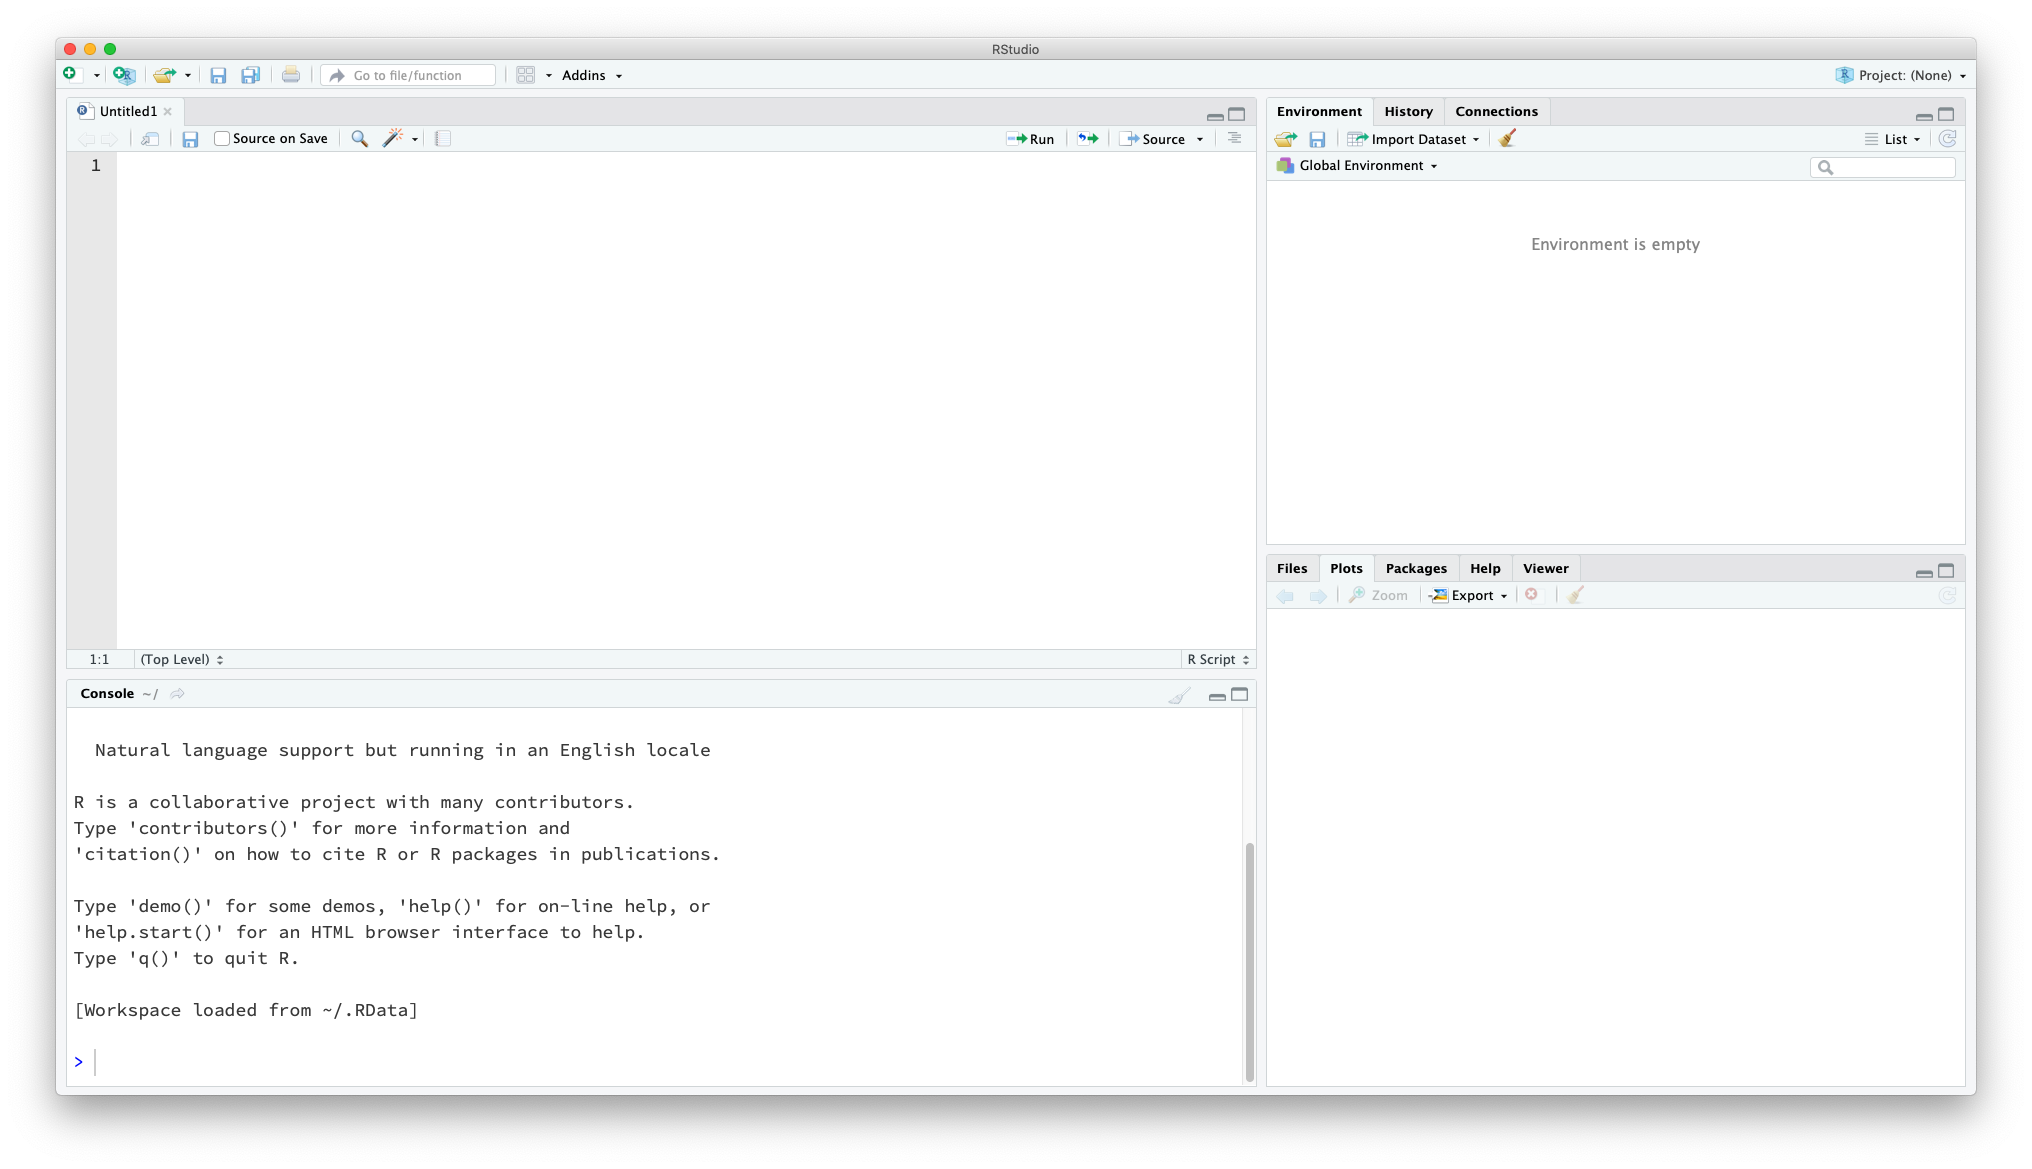
\includegraphics[width=5.20833in,height=\textheight]{fig/rstudio.png}

}

\end{figure}

这是一个非常干净的RStudio的界面。左上角的部分是源文件窗口,用来阅读和书写代码;左下角的部分是控制台(console),用来输出代码的运行结果;右上角的窗口罗列了当前环境(environment)中的对象(objects),也可以用来查看已执行的代码;右下角的窗口整合了文件、图像、包(packages)、帮助等功能。

RStudio
提供了一些实用的快捷键,现阶段我们只需要记住一个:\texttt{Ctrl/Cmd\ +\ Enter}运行选中代码。

\hypertarget{ux914dux7f6e-copilot}{%
\section{配置 Copilot}\label{ux914dux7f6e-copilot}}

AI时代,写代码不能少了Copilot。请参考这篇\href{https://mp.weixin.qq.com/s/YA5LNely0alemNfX0Upoew}{公众号文章},在RStudio中配置Copilot。它可以帮你自动补全代码。

Copilot
有很多使用方法,其核心逻辑是通过\textbf{代码文件中现有的内容}来预测你接下来想写的东西。比方说,如果你想批量地对数据中的变量名做某一种操作,那么大约有下列步骤:

\begin{enumerate}
\def\labelenumi{\arabic{enumi}.}
\tightlist
\item
  打印数据的变量名列表
\item
  把数据的变量名列表粘贴到代码文件中
\item
  写1-2行代码示例
\item
  等待 Copilot 自动补全,然后按 tab 键同意
\item
  把光标移到整段代码的上方,键入井号(\#),让 Copilot 自动生成注释
\end{enumerate}

注意,一般来说,Copilot
只会填补句尾、整行或整段的空白。换句话说,你需要把光标移动到句末或者空白行,它才会开始运转。当光标在句中或句首时,别再痴痴地等着它来填补啦。

\hypertarget{ux7b80ux5355ux7684ux4ee3ux7801}{%
\section{简单的代码}\label{ux7b80ux5355ux7684ux4ee3ux7801}}

安装好了 R 和
RStudio,我们就可以尝试一些简单的代码了。比方说,我们可以在 R
里面直接进行四则运算:

\begin{Shaded}
\begin{Highlighting}[]
\DecValTok{1} \SpecialCharTok{+} \DecValTok{1}
\end{Highlighting}
\end{Shaded}

\begin{verbatim}
[1] 2
\end{verbatim}

\begin{Shaded}
\begin{Highlighting}[]
\CommentTok{\# 用 3, 4, 5, 9 算 24 点}
\NormalTok{(}\DecValTok{4} \SpecialCharTok{+} \DecValTok{9} \SpecialCharTok{{-}} \DecValTok{5}\NormalTok{) }\SpecialCharTok{*} \DecValTok{3}
\end{Highlighting}
\end{Shaded}

\begin{verbatim}
[1] 24
\end{verbatim}

在 R 里面,可以用引号包裹多语言文本:

\begin{Shaded}
\begin{Highlighting}[]
\CommentTok{\# 使用英文的单引号 \textquotesingle{}\textquotesingle{} 或双引号 "" 表示文本}
\StringTok{"你好,R!"}
\end{Highlighting}
\end{Shaded}

\begin{verbatim}
[1] "你好,R!"
\end{verbatim}

也可以调用函数完成更复杂的任务:

\begin{Shaded}
\begin{Highlighting}[]
\CommentTok{\# 用 sqrt() 开平方根}
\FunctionTok{sqrt}\NormalTok{(}\DecValTok{25}\NormalTok{)}
\end{Highlighting}
\end{Shaded}

\begin{verbatim}
[1] 5
\end{verbatim}

\begin{Shaded}
\begin{Highlighting}[]
\CommentTok{\# 用 nchar() 数字符数}
\FunctionTok{nchar}\NormalTok{(}\StringTok{"你好"}\NormalTok{)}
\end{Highlighting}
\end{Shaded}

\begin{verbatim}
[1] 2
\end{verbatim}

此外,我们可以把一些结果存储下来,以便后期调用:

\begin{Shaded}
\begin{Highlighting}[]
\CommentTok{\# 赋值 a 为 123}
\NormalTok{a }\OtherTok{\textless{}{-}} \DecValTok{123}
\CommentTok{\# 查看 a 的值}
\NormalTok{a}
\end{Highlighting}
\end{Shaded}

\begin{verbatim}
[1] 123
\end{verbatim}

\begin{Shaded}
\begin{Highlighting}[]
\CommentTok{\# 计算 a 乘以 2}
\NormalTok{a }\SpecialCharTok{*} \DecValTok{2}
\end{Highlighting}
\end{Shaded}

\begin{verbatim}
[1] 246
\end{verbatim}

\begin{Shaded}
\begin{Highlighting}[]
\CommentTok{\# 赋值 b 为 a 乘以 2 的结果}
\NormalTok{b }\OtherTok{\textless{}{-}}\NormalTok{ a }\SpecialCharTok{*} \DecValTok{2}
\CommentTok{\# 查看 b 的值}
\NormalTok{b}
\end{Highlighting}
\end{Shaded}

\begin{verbatim}
[1] 246
\end{verbatim}

\hypertarget{ux5b89ux88c5-r-ux5305}{%
\section{安装 R 包}\label{ux5b89ux88c5-r-ux5305}}

在本书中,我们主要需要用到 tidyverse 包和 statart
包。在继续下面的内容之前,请让我们先下载这两个包:

\begin{Shaded}
\begin{Highlighting}[]
\CommentTok{\# 下载 tidyverse}
\FunctionTok{install.packages}\NormalTok{(}\StringTok{"tidyverse"}\NormalTok{)}
\CommentTok{\# 下载 statart}
\NormalTok{devtools}\SpecialCharTok{::}\FunctionTok{install\_github}\NormalTok{(}\StringTok{"socimh/statart"}\NormalTok{)}
\end{Highlighting}
\end{Shaded}

\hypertarget{ux5bf9ux8c61ux548cux7c7bux578b}{%
\section{对象和类型}\label{ux5bf9ux8c61ux548cux7c7bux578b}}

好,在刚才的例子里,我们其实接触了很多 R
里面的对象(object)。我们可以使用 statart 包里的 \texttt{s\_type()}
函数来判断对象的类型(type):

\begin{Shaded}
\begin{Highlighting}[]
\FunctionTok{library}\NormalTok{(statart)}
\end{Highlighting}
\end{Shaded}

\begin{Shaded}
\begin{Highlighting}[]
\CommentTok{\# 实数(double)}
\FunctionTok{s\_type}\NormalTok{(}\DecValTok{25}\NormalTok{)}
\end{Highlighting}
\end{Shaded}

\begin{verbatim}
[1] "double"
\end{verbatim}

\begin{Shaded}
\begin{Highlighting}[]
\CommentTok{\# 字符(character)}
\FunctionTok{s\_type}\NormalTok{(}\StringTok{"你好,R!"}\NormalTok{)}
\end{Highlighting}
\end{Shaded}

\begin{verbatim}
[1] "character"
\end{verbatim}

\begin{Shaded}
\begin{Highlighting}[]
\CommentTok{\# 函数(function)}
\FunctionTok{s\_type}\NormalTok{(sqrt)}
\end{Highlighting}
\end{Shaded}

\begin{verbatim}
[1] "function"
\end{verbatim}

函数通常都以 \texttt{f()} 的形式出现,带有圆括号。

\hypertarget{ux6570ux636eux548cux51fdux6570}{%
\section{数据和函数}\label{ux6570ux636eux548cux51fdux6570}}

所以,在前面一小节的几行代码里,我们已经接触了实数(double)、字符(character)和函数(function)这三种对象了。反过来说,上述代码基本都是由对象组成的。

我们可以把对象大致分为数据(data)和函数。广义的``数据''类似于信息(information),比方说
\texttt{25} 和
\texttt{"你好"},只要有实际内容就行。当然,这和我们日常生活中的用法有所不同。我眼中的数据,可以涵盖衣食住行等我们生活中任何有实际意义的东西。

\begin{tcolorbox}[enhanced jigsaw, bottomtitle=1mm, bottomrule=.15mm, coltitle=black, title=\textcolor{quarto-callout-note-color}{\faInfo}\hspace{0.5em}{笔记}, toptitle=1mm, colframe=quarto-callout-note-color-frame, colbacktitle=quarto-callout-note-color!10!white, opacitybacktitle=0.6, arc=.35mm, opacityback=0, breakable, toprule=.15mm, left=2mm, titlerule=0mm, rightrule=.15mm, colback=white, leftrule=.75mm]

所有信息,都可以是数据。

\end{tcolorbox}

如果代码中只有数据,那它通常做不了什么。打个比方,数据就像是名词,而一堆名词是零散的,无法组成句子。``头、明月、头、故乡'',这不成一句话;``举头望明月,低头思故乡''有了动词的``润滑'',就可以串联成一句话了。函数就像是动词。

\begin{tcolorbox}[enhanced jigsaw, bottomtitle=1mm, bottomrule=.15mm, coltitle=black, title=\textcolor{quarto-callout-note-color}{\faInfo}\hspace{0.5em}{笔记}, toptitle=1mm, colframe=quarto-callout-note-color-frame, colbacktitle=quarto-callout-note-color!10!white, opacitybacktitle=0.6, arc=.35mm, opacityback=0, breakable, toprule=.15mm, left=2mm, titlerule=0mm, rightrule=.15mm, colback=white, leftrule=.75mm]

在 R 语言里,数据(data)通常像名词,而函数(functions)通常像动词。

\end{tcolorbox}

\hypertarget{ux6570ux636eux7684ux7ef4ux5ea6}{%
\section{数据的维度}\label{ux6570ux636eux7684ux7ef4ux5ea6}}

R
语言是一门分析数据的语言。但是,数据的种类那么多,我们要如何上手呢?我想从数据的维度说起。

随着 3D 电影和 VR 设备的普及,我们可以看到三维立体的视频。3D 的 D
就是维度(dimension)的意思。在我看来,我们常用的数据也有四种维度:零维、一维、二维和多维。

维度

几何意义

数据意义

R 语言范例

零维(0D)

点

值

数、字符等

一维(1D)

线

列

数列、字符向量等

二维(2D)

面

表格

矩阵、tibble等

多维(nD)

多维空间

数组(array)

数组、多级列表等

零维的数据就是值。比方说,我们讲中国有14亿人,``14亿''就是一个零维的数据;广东简称``粤'',则``粤''这个字也可以视作零维的数据。

一维的数据是列,或者说多个值的集合。这在我们生活中很常见。比方说,1到10的数列就是一维的数据;再比如,中国所有省份的名称,就构成一列字符,或者叫字符向量(character
vector)。

二维的数据是表,或者说多列的集合。这也是我们生活中最常见的数据维度,像
Excel 一打开就是二维数据的处理面板。这里不做赘述。

多维的数据是数组,是由低维数据一层层集合上来得到的。一个例子是时间:秒、分、时、天、月、年,向上集合,最终组成了一个六维的数据。年包括月,月包括天,以此类推。我们说``2008年8月8日
20时00分00秒'',其实就是指定了六个维度,指向时间的六维空间中特定的那一个时点------北京奥运会开幕的那个瞬间。

\begin{figure}

{\centering 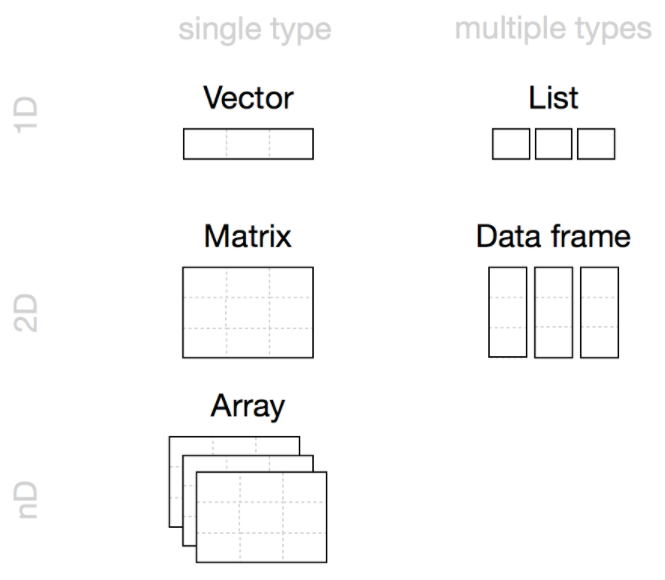
\includegraphics[width=4.16667in,height=\textheight]{fig/types.png}

}

\end{figure}

\hypertarget{r-ux5de5ux4f5cux6d41ux7a0b}{%
\section{R 工作流程}\label{r-ux5de5ux4f5cux6d41ux7a0b}}

显然,我们做统计分析时,最常接触的就是一维和二维的数据。但是在 R
里面,一维和二维的数据仍然有很多类型,我们应该从何学起呢?

我认为,只要先把 tibble 摸透,就可以完成大多数数据分析了。

\begin{figure}

{\centering 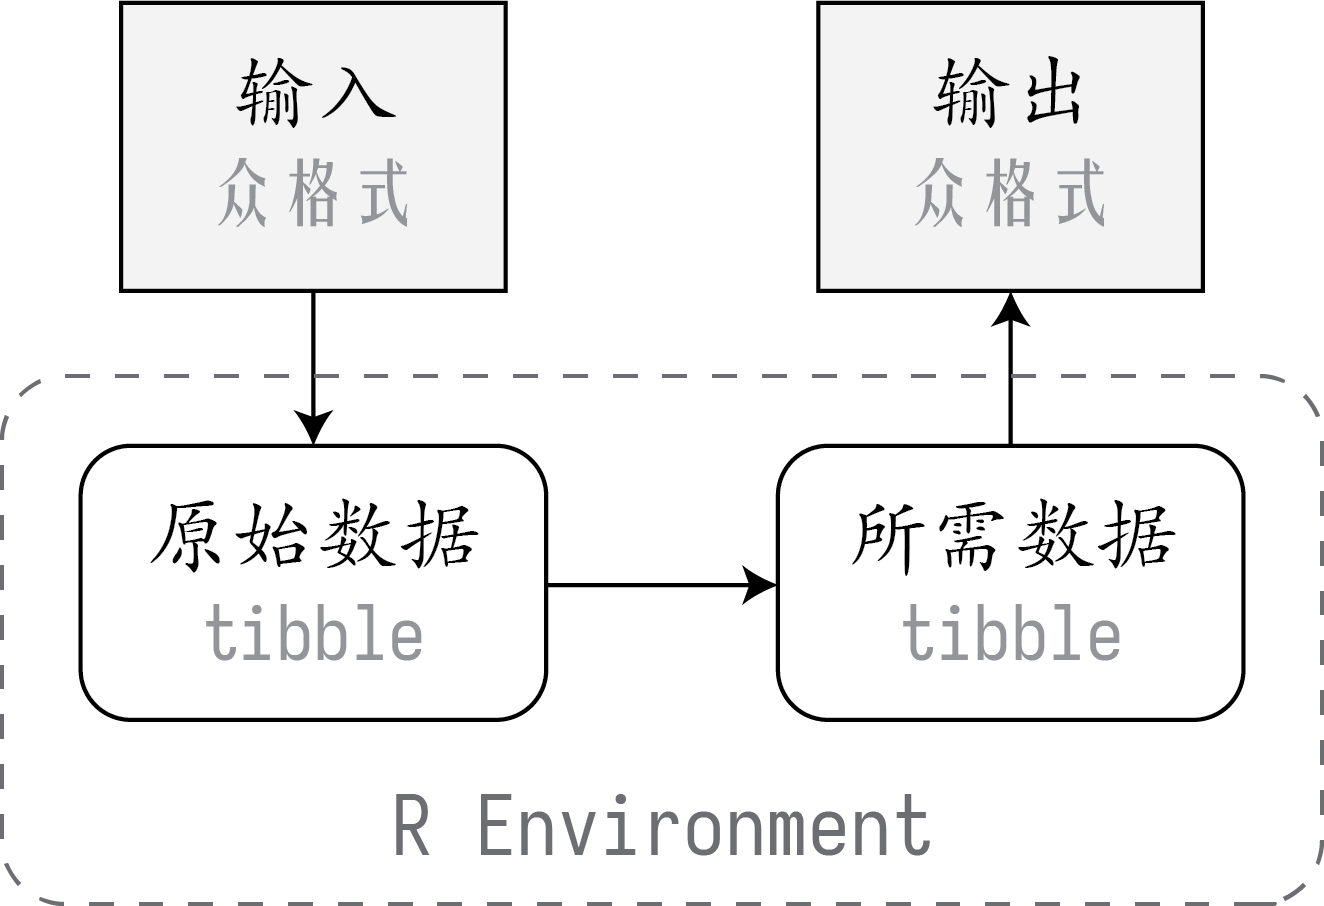
\includegraphics[width=4.16667in,height=\textheight]{fig/intro_diagram.png}

}

\end{figure}

当然,输入和输出的数据,通常都不是
tibble。但是,只需要三个步骤,我们就可以把任意格式的输入数据转换成任意格式的输出内容了。

\begin{enumerate}
\def\labelenumi{\arabic{enumi}.}
\tightlist
\item
  将其他格式数据导入为 tibble
\item
  处理 tibble
\item
  将 tibble 数据导出为其他格式
\end{enumerate}

这里,输入的数据格式可以是

\begin{itemize}
\tightlist
\item
  .RData 和 .rds 等 R 格式的数据
\item
  R 和 R 包自带数据
\item
  通过 R 代码手动输入的数据
\item
  Excel 数据
\item
  Stata, SPSS, SAS 等统计软件数据
\item
  .csv, .tsv, .txt 等纯文本数据
\item
  .zip, .gz, .bz2, .xz 等压缩数据
\item
  .bin, .dat, .ftr, .parquet 等二进制数据
\item
  XML, HTML, JSON 等标记数据
\item
  .shp, .geotiff 等地理信息数据
\item
  文件夹、压缩包
\item
  图片
\item
  远程数据库和大数据
\item
  在线数据、网站源码等
\item
  还有很多\ldots{}
\end{itemize}

类似地,R
不仅可以导出成\textbf{上面大部分格式}的数据,而且可以直接输出统计报告,包括

\begin{itemize}
\tightlist
\item
  在终端输出的文本和表格(复制或截图)
\item
  Excel, Markdown, LaTeX 等格式的表格
\item
  各种格式的图片
\item
  Word 和 PDF 文档
\item
  html 网页
\item
  可交互的图表
\item
  (配合 Quarto)幻灯片
\item
  (配合 Quarto)文章、书籍等
\item
  (配合 Quarto)网站
\item
  还有很多\ldots{}
\end{itemize}

可见,学会了 tibble 这个桥梁,我们能够完成多少任务!

\hypertarget{sec-chengyu}{%
\section{成语接龙}\label{sec-chengyu}}

\begin{figure}

\begin{minipage}[t]{0.50\linewidth}

{\centering 

\raisebox{-\height}{

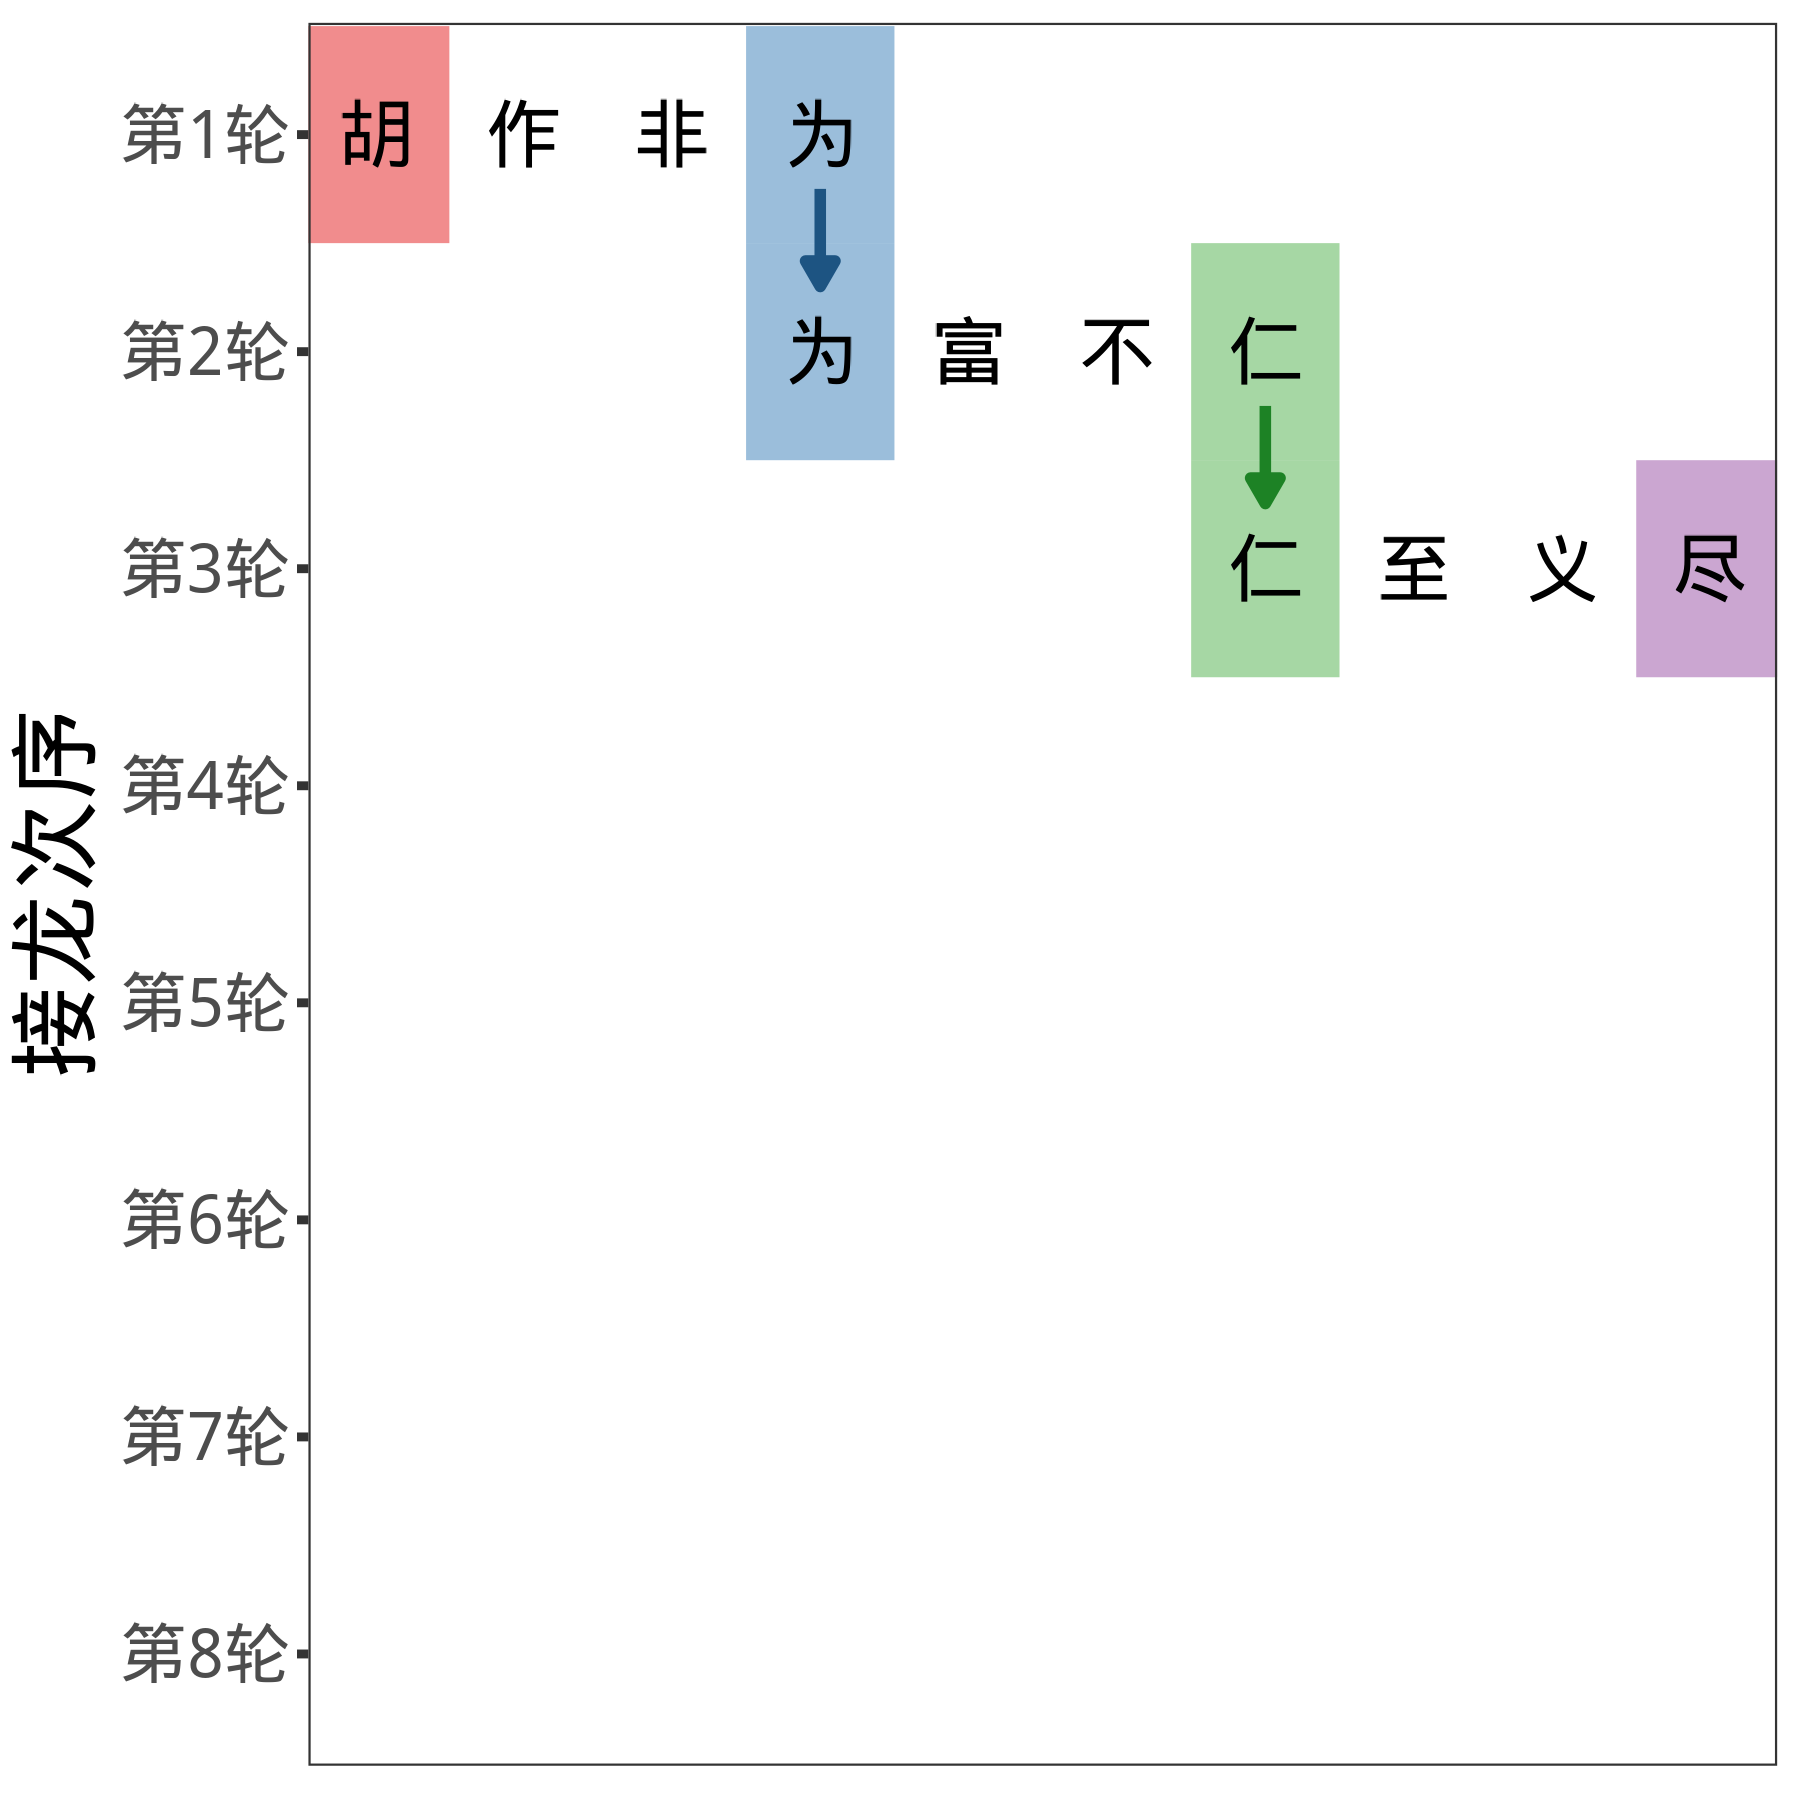
\includegraphics{fig/word_chain_short.png}

}

\caption{\label{fig-short}普通的成语接龙}

}

\end{minipage}%
%
\begin{minipage}[t]{0.50\linewidth}

{\centering 

\raisebox{-\height}{

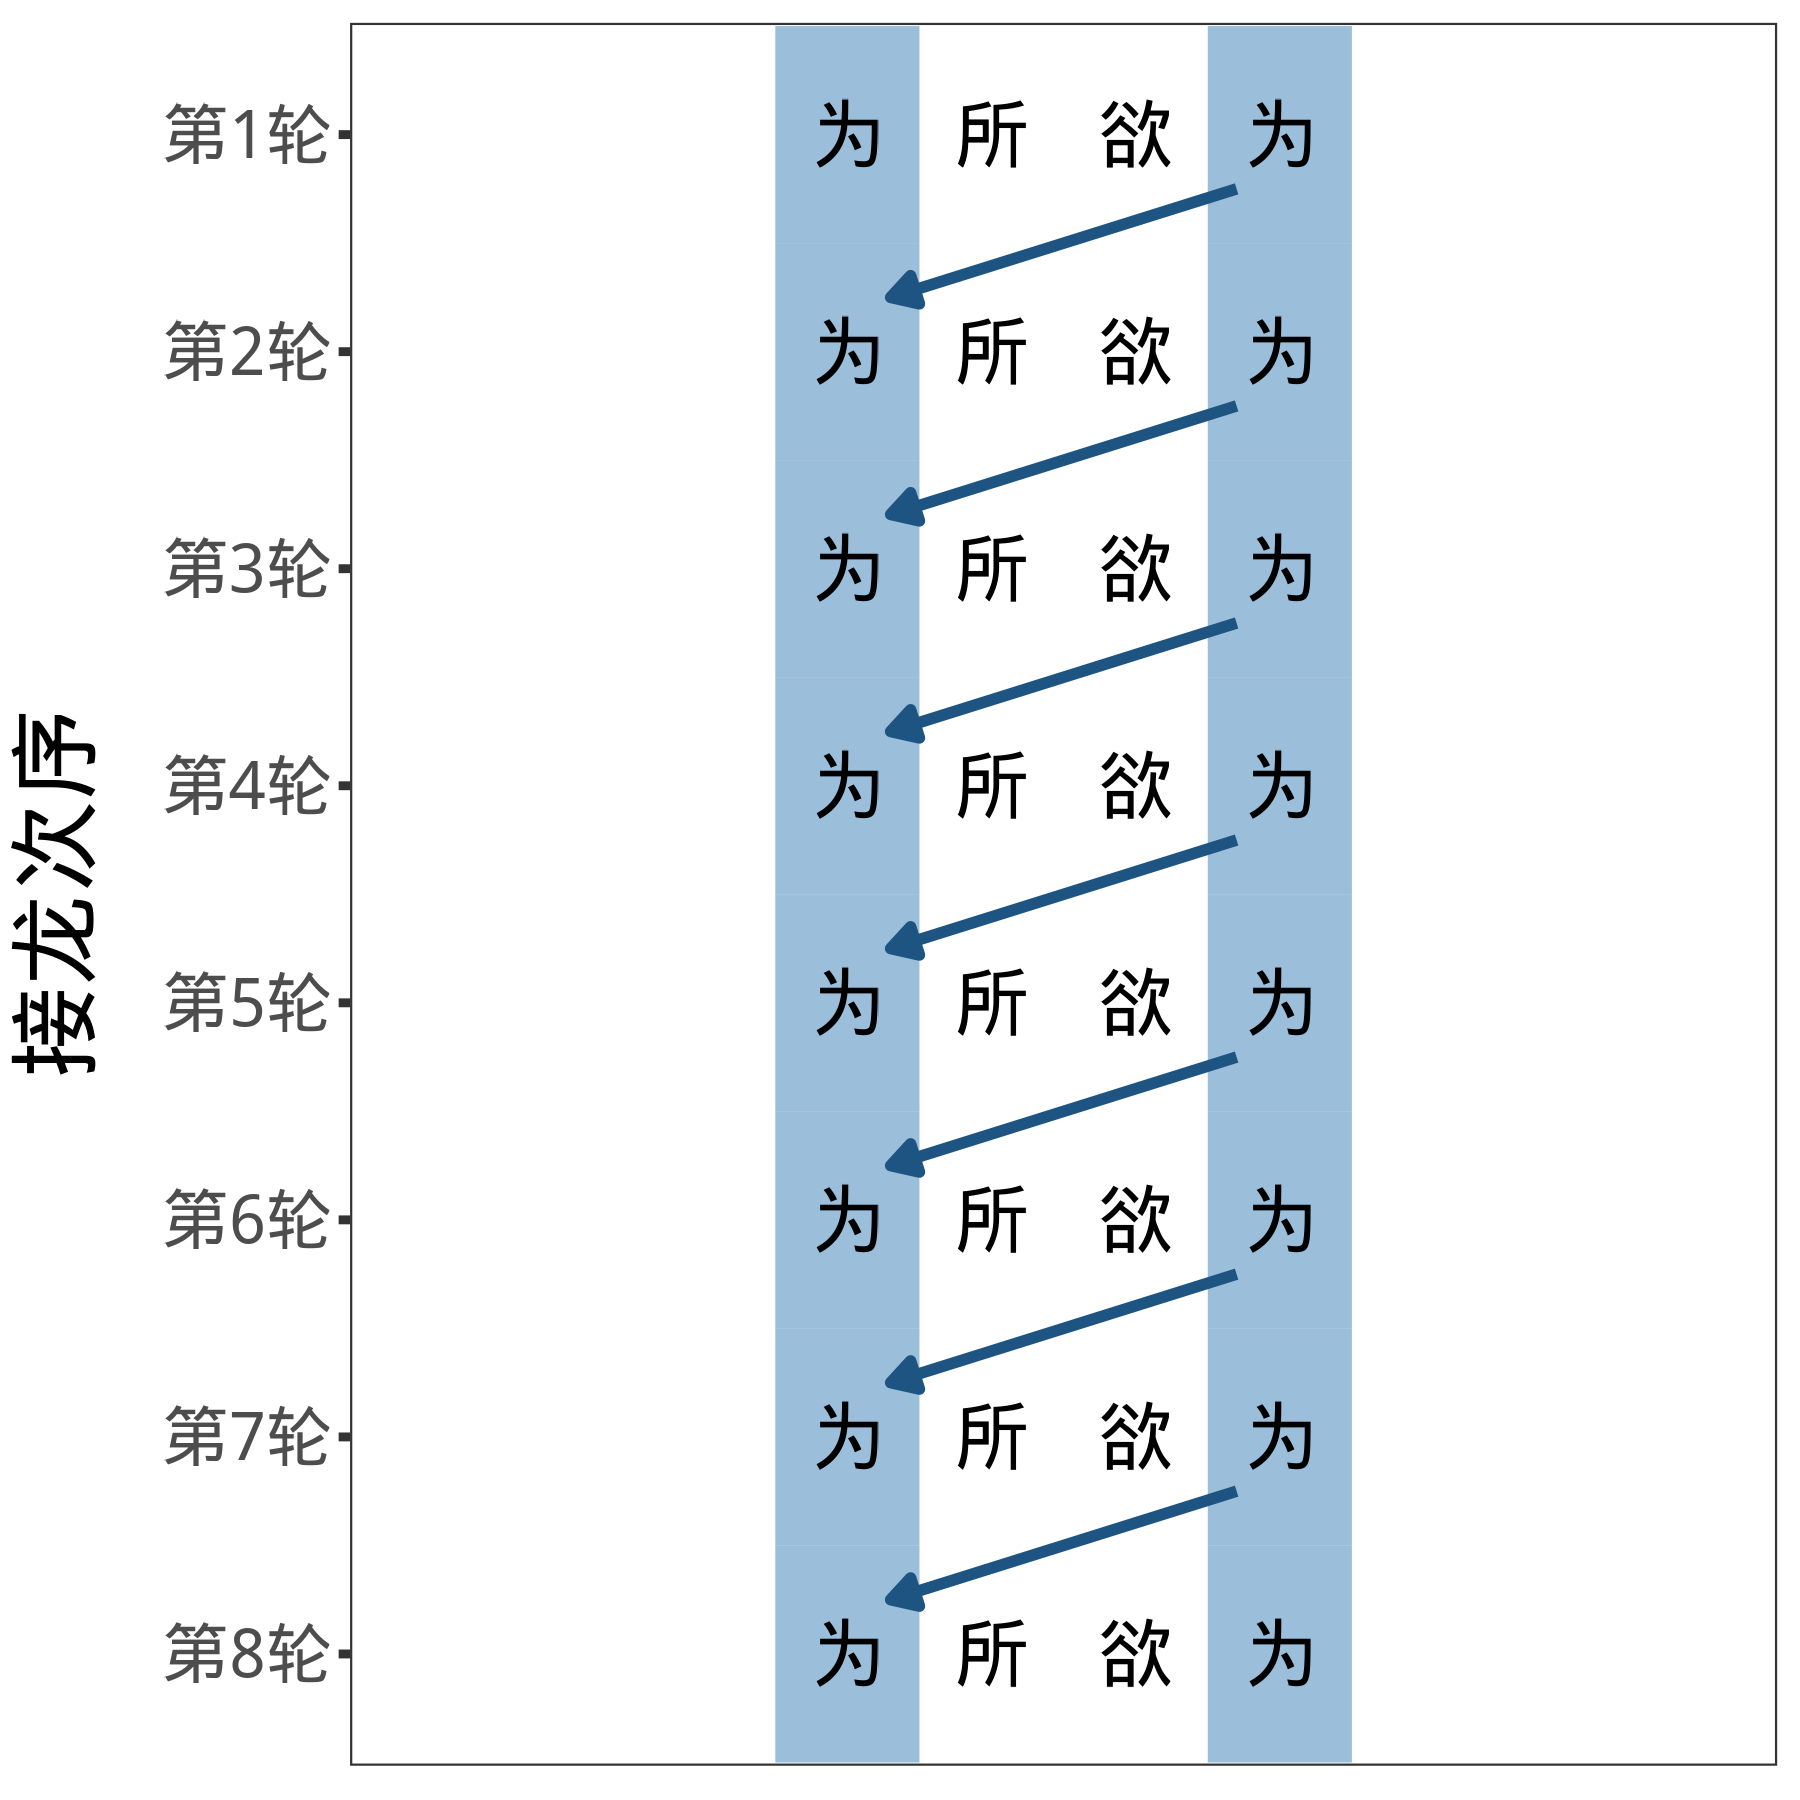
\includegraphics{fig/word_chain_long.png}

}

\caption{\label{fig-long}``为所欲为''的成语接龙}

}

\end{minipage}%

\end{figure}

用成语接龙打个比方,大部分成语输入的字和输出的字都不一样。但是,``为所欲为''却是一个例外,输入的是``为'',输出的也是``为''。学会``为所欲为''的小朋友,哪怕成语储备量只有这一个,也能自己接龙100次。(详见
章节~\ref{sec-wei} )

我们工作坊要学的,99\%的函数都会围绕 tibble 和
gg;这是我的刻意设计,也是大势所趋。

我对R的初学者有三个建议:

\begin{enumerate}
\def\labelenumi{\arabic{enumi}.}
\tightlist
\item
  只学 tibble,不必分心学向量(vector)、列表(list)、矩阵、data.table
  等对象
\item
  只学可能要用的,忘记一定没用的
\item
  无需死记硬背,想用什么查一下,用多了自然就记住了
\end{enumerate}

其实我自己现在也是这样。data.table
怎么用,早就忘得差不多了;想要处理一个复杂的 list,有的 purrr
函数,也得临时去查。不过一旦入门了,这种简单的函数,一两分钟就会用了。

\hypertarget{ux5bfcux5165ux5bfcux51faux6570ux636e}{%
\section{导入导出数据}\label{ux5bfcux5165ux5bfcux51faux6570ux636e}}

\begin{itemize}
\tightlist
\item
  \texttt{Week1-1.\ import\_and\_export\_dta.R}
  简要地演示了清理数据的全流程
\item
  \texttt{Week1-2.\ import\_and\_plot\_dta.R}
  简要地演示了数据可视化的全流程
\item
  \texttt{Week1-3.\ import\_any\_data.R} 展示了如何导入各种类型的数据
\item
  \texttt{Week1-4.\ generate\_and\_export\_any\_data.R}
  展示了如何生成、导出各种类型的数据
\end{itemize}

\bookmarksetup{startatroot}

\hypertarget{tibble-ux6570ux636e}{%
\chapter{tibble 数据}\label{tibble-ux6570ux636e}}

\hypertarget{ux6574ux6d01ux6570ux636e}{%
\section{整洁数据}\label{ux6574ux6d01ux6570ux636e}}

在浩如烟海的数据类型中,有一种数据类型特别为统计学家所关注。这一类数据有如下特点:

\begin{enumerate}
\def\labelenumi{\arabic{enumi}.}
\tightlist
\item
  每行是一个个案(case)、个体(individual)、观测点(observation)、分析单位(unit
  of analysis)

  \begin{itemize}
  \tightlist
  \item
    统计上讲,这些概念等价
  \end{itemize}
\item
  每列是一个变量(variable)、特征(feature)
\item
  每格是一个取值(value),即某个个案的某条特征
\end{enumerate}

这一类数据,有一种说法是整洁数据(tidy
data),和其他五花八门的杂乱数据(messy data)相对。

整洁数据的结构非常清晰,通过行和列,可以锁定每个格子数值的含义。

下面是一些整洁数据的示例:

\begin{longtable}[]{@{}
  >{\raggedright\arraybackslash}p{(\columnwidth - 14\tabcolsep) * \real{0.1899}}
  >{\raggedleft\arraybackslash}p{(\columnwidth - 14\tabcolsep) * \real{0.0886}}
  >{\raggedleft\arraybackslash}p{(\columnwidth - 14\tabcolsep) * \real{0.0633}}
  >{\raggedright\arraybackslash}p{(\columnwidth - 14\tabcolsep) * \real{0.1519}}
  >{\raggedright\arraybackslash}p{(\columnwidth - 14\tabcolsep) * \real{0.1519}}
  >{\raggedright\arraybackslash}p{(\columnwidth - 14\tabcolsep) * \real{0.1266}}
  >{\raggedleft\arraybackslash}p{(\columnwidth - 14\tabcolsep) * \real{0.1392}}
  >{\raggedright\arraybackslash}p{(\columnwidth - 14\tabcolsep) * \real{0.0886}}@{}}
\caption{一、starwars 星球大战角色数据(87行,14列)}\tabularnewline
\toprule\noalign{}
\begin{minipage}[b]{\linewidth}\raggedright
name
\end{minipage} & \begin{minipage}[b]{\linewidth}\raggedleft
height
\end{minipage} & \begin{minipage}[b]{\linewidth}\raggedleft
mass
\end{minipage} & \begin{minipage}[b]{\linewidth}\raggedright
hair\_color
\end{minipage} & \begin{minipage}[b]{\linewidth}\raggedright
skin\_color
\end{minipage} & \begin{minipage}[b]{\linewidth}\raggedright
eye\_color
\end{minipage} & \begin{minipage}[b]{\linewidth}\raggedleft
birth\_year
\end{minipage} & \begin{minipage}[b]{\linewidth}\raggedright
sex
\end{minipage} \\
\midrule\noalign{}
\endfirsthead
\toprule\noalign{}
\begin{minipage}[b]{\linewidth}\raggedright
name
\end{minipage} & \begin{minipage}[b]{\linewidth}\raggedleft
height
\end{minipage} & \begin{minipage}[b]{\linewidth}\raggedleft
mass
\end{minipage} & \begin{minipage}[b]{\linewidth}\raggedright
hair\_color
\end{minipage} & \begin{minipage}[b]{\linewidth}\raggedright
skin\_color
\end{minipage} & \begin{minipage}[b]{\linewidth}\raggedright
eye\_color
\end{minipage} & \begin{minipage}[b]{\linewidth}\raggedleft
birth\_year
\end{minipage} & \begin{minipage}[b]{\linewidth}\raggedright
sex
\end{minipage} \\
\midrule\noalign{}
\endhead
\bottomrule\noalign{}
\endlastfoot
Luke Skywalker & 172 & 77 & blond & fair & blue & 19.0 & male \\
C-3PO & 167 & 75 & NA & gold & yellow & 112.0 & none \\
R2-D2 & 96 & 32 & NA & white, blue & red & 33.0 & none \\
Darth Vader & 202 & 136 & none & white & yellow & 41.9 & male \\
Leia Organa & 150 & 49 & brown & light & brown & 19.0 & female \\
Owen Lars & 178 & 120 & brown, grey & light & blue & 52.0 & male \\
\end{longtable}

\begin{longtable}[]{@{}
  >{\raggedright\arraybackslash}p{(\columnwidth - 14\tabcolsep) * \real{0.1857}}
  >{\raggedright\arraybackslash}p{(\columnwidth - 14\tabcolsep) * \real{0.3429}}
  >{\raggedright\arraybackslash}p{(\columnwidth - 14\tabcolsep) * \real{0.1857}}
  >{\raggedleft\arraybackslash}p{(\columnwidth - 14\tabcolsep) * \real{0.0571}}
  >{\raggedleft\arraybackslash}p{(\columnwidth - 14\tabcolsep) * \real{0.0571}}
  >{\raggedleft\arraybackslash}p{(\columnwidth - 14\tabcolsep) * \real{0.0571}}
  >{\raggedleft\arraybackslash}p{(\columnwidth - 14\tabcolsep) * \real{0.0571}}
  >{\raggedleft\arraybackslash}p{(\columnwidth - 14\tabcolsep) * \real{0.0571}}@{}}
\caption{二、billboard 歌曲榜单数据(79行,317列)}\tabularnewline
\toprule\noalign{}
\begin{minipage}[b]{\linewidth}\raggedright
artist
\end{minipage} & \begin{minipage}[b]{\linewidth}\raggedright
track
\end{minipage} & \begin{minipage}[b]{\linewidth}\raggedright
date.entered
\end{minipage} & \begin{minipage}[b]{\linewidth}\raggedleft
wk1
\end{minipage} & \begin{minipage}[b]{\linewidth}\raggedleft
wk2
\end{minipage} & \begin{minipage}[b]{\linewidth}\raggedleft
wk3
\end{minipage} & \begin{minipage}[b]{\linewidth}\raggedleft
wk4
\end{minipage} & \begin{minipage}[b]{\linewidth}\raggedleft
wk5
\end{minipage} \\
\midrule\noalign{}
\endfirsthead
\toprule\noalign{}
\begin{minipage}[b]{\linewidth}\raggedright
artist
\end{minipage} & \begin{minipage}[b]{\linewidth}\raggedright
track
\end{minipage} & \begin{minipage}[b]{\linewidth}\raggedright
date.entered
\end{minipage} & \begin{minipage}[b]{\linewidth}\raggedleft
wk1
\end{minipage} & \begin{minipage}[b]{\linewidth}\raggedleft
wk2
\end{minipage} & \begin{minipage}[b]{\linewidth}\raggedleft
wk3
\end{minipage} & \begin{minipage}[b]{\linewidth}\raggedleft
wk4
\end{minipage} & \begin{minipage}[b]{\linewidth}\raggedleft
wk5
\end{minipage} \\
\midrule\noalign{}
\endhead
\bottomrule\noalign{}
\endlastfoot
2 Pac & Baby Don't Cry (Keep\ldots{} & 2000-02-26 & 87 & 82 & 72 & 77 &
87 \\
2Ge+her & The Hardest Part Of \ldots{} & 2000-09-02 & 91 & 87 & 92 & NA
& NA \\
3 Doors Down & Kryptonite & 2000-04-08 & 81 & 70 & 68 & 67 & 66 \\
3 Doors Down & Loser & 2000-10-21 & 76 & 76 & 72 & 69 & 67 \\
504 Boyz & Wobble Wobble & 2000-04-15 & 57 & 34 & 25 & 17 & 17 \\
98\^{}0 & Give Me Just One Nig\ldots{} & 2000-08-19 & 51 & 39 & 34 & 26
& 26 \\
\end{longtable}

\begin{longtable}[]{@{}
  >{\raggedleft\arraybackslash}p{(\columnwidth - 18\tabcolsep) * \real{0.0952}}
  >{\raggedright\arraybackslash}p{(\columnwidth - 18\tabcolsep) * \real{0.1587}}
  >{\raggedright\arraybackslash}p{(\columnwidth - 18\tabcolsep) * \real{0.0952}}
  >{\raggedright\arraybackslash}p{(\columnwidth - 18\tabcolsep) * \real{0.1270}}
  >{\raggedleft\arraybackslash}p{(\columnwidth - 18\tabcolsep) * \real{0.0952}}
  >{\raggedleft\arraybackslash}p{(\columnwidth - 18\tabcolsep) * \real{0.0952}}
  >{\raggedleft\arraybackslash}p{(\columnwidth - 18\tabcolsep) * \real{0.0952}}
  >{\raggedleft\arraybackslash}p{(\columnwidth - 18\tabcolsep) * \real{0.0794}}
  >{\raggedleft\arraybackslash}p{(\columnwidth - 18\tabcolsep) * \real{0.0794}}
  >{\raggedleft\arraybackslash}p{(\columnwidth - 18\tabcolsep) * \real{0.0794}}@{}}
\caption{三、diamonds 钻石数据(53940行,10列)}\tabularnewline
\toprule\noalign{}
\begin{minipage}[b]{\linewidth}\raggedleft
carat
\end{minipage} & \begin{minipage}[b]{\linewidth}\raggedright
cut
\end{minipage} & \begin{minipage}[b]{\linewidth}\raggedright
color
\end{minipage} & \begin{minipage}[b]{\linewidth}\raggedright
clarity
\end{minipage} & \begin{minipage}[b]{\linewidth}\raggedleft
depth
\end{minipage} & \begin{minipage}[b]{\linewidth}\raggedleft
table
\end{minipage} & \begin{minipage}[b]{\linewidth}\raggedleft
price
\end{minipage} & \begin{minipage}[b]{\linewidth}\raggedleft
x
\end{minipage} & \begin{minipage}[b]{\linewidth}\raggedleft
y
\end{minipage} & \begin{minipage}[b]{\linewidth}\raggedleft
z
\end{minipage} \\
\midrule\noalign{}
\endfirsthead
\toprule\noalign{}
\begin{minipage}[b]{\linewidth}\raggedleft
carat
\end{minipage} & \begin{minipage}[b]{\linewidth}\raggedright
cut
\end{minipage} & \begin{minipage}[b]{\linewidth}\raggedright
color
\end{minipage} & \begin{minipage}[b]{\linewidth}\raggedright
clarity
\end{minipage} & \begin{minipage}[b]{\linewidth}\raggedleft
depth
\end{minipage} & \begin{minipage}[b]{\linewidth}\raggedleft
table
\end{minipage} & \begin{minipage}[b]{\linewidth}\raggedleft
price
\end{minipage} & \begin{minipage}[b]{\linewidth}\raggedleft
x
\end{minipage} & \begin{minipage}[b]{\linewidth}\raggedleft
y
\end{minipage} & \begin{minipage}[b]{\linewidth}\raggedleft
z
\end{minipage} \\
\midrule\noalign{}
\endhead
\bottomrule\noalign{}
\endlastfoot
0.23 & Ideal & E & SI2 & 61.5 & 55 & 326 & 3.95 & 3.98 & 2.43 \\
0.21 & Premium & E & SI1 & 59.8 & 61 & 326 & 3.89 & 3.84 & 2.31 \\
0.23 & Good & E & VS1 & 56.9 & 65 & 327 & 4.05 & 4.07 & 2.31 \\
0.29 & Premium & I & VS2 & 62.4 & 58 & 334 & 4.20 & 4.23 & 2.63 \\
0.31 & Good & J & SI2 & 63.3 & 58 & 335 & 4.34 & 4.35 & 2.75 \\
0.24 & Very Good & J & VVS2 & 62.8 & 57 & 336 & 3.94 & 3.96 & 2.48 \\
\end{longtable}

\hypertarget{tidyverse}{%
\section{\texorpdfstring{\texttt{tidyverse}}{tidyverse}}\label{tidyverse}}

本文是对 tidyverse 的入门介绍。

tidyverse
(直译为``整洁宇宙'\,')整合了一系列主要处理、分析整洁数据的R包(R
packages)。每个包里面都有大量的函数。其特点是函数的命名、语法、用法非常整洁统一。

\begin{Shaded}
\begin{Highlighting}[]
\CommentTok{\# 加载 tidyverse 包}
\FunctionTok{library}\NormalTok{(tidyverse)}
\end{Highlighting}
\end{Shaded}

\begin{verbatim}
Warning: package 'ggplot2' was built under R version 4.3.3
\end{verbatim}

\begin{verbatim}
Warning: package 'stringr' was built under R version 4.3.2
\end{verbatim}

\begin{verbatim}
-- Attaching core tidyverse packages ------------------------ tidyverse 2.0.0 --
v dplyr     1.1.2     v readr     2.1.4
v forcats   1.0.0     v stringr   1.5.1
v ggplot2   3.5.1     v tibble    3.2.1
v lubridate 1.9.2     v tidyr     1.3.0
v purrr     1.0.1     
-- Conflicts ------------------------------------------ tidyverse_conflicts() --
x tidyr::extract()   masks magrittr::extract()
x dplyr::filter()    masks stats::filter()
x dplyr::lag()       masks stats::lag()
x purrr::set_names() masks magrittr::set_names()
i Use the conflicted package (<http://conflicted.r-lib.org/>) to force all conflicts to become errors
\end{verbatim}

\begin{tcolorbox}[enhanced jigsaw, bottomtitle=1mm, bottomrule=.15mm, coltitle=black, title=\textcolor{quarto-callout-tip-color}{\faLightbulb}\hspace{0.5em}{提示}, toptitle=1mm, colframe=quarto-callout-tip-color-frame, colbacktitle=quarto-callout-tip-color!10!white, opacitybacktitle=0.6, arc=.35mm, opacityback=0, breakable, toprule=.15mm, left=2mm, titlerule=0mm, rightrule=.15mm, colback=white, leftrule=.75mm]

在载入 tidyverse 时,可能会出现类似上面的一些警告语,它们不会影响
tidyverse 的正常使用,请无须担心。

\end{tcolorbox}

tidyverse 为整洁数据设计了一种数据格式,叫作 tibble。这个词是 tidy 和
table
的结合,顾名思义,特指整洁数据。它相当于Excel里的表格(整洁的才行)、Stata
里的数据、Python 里的 Pandas 数据框等。

\textbf{在数据科学中,整洁数据是最主流的数据形式。}尽管我们日常生活中,可以看到形形色色的数据呈现形式(比如12306列车时间表、网购的商品列表等),但是它们的底层数据都是很整洁的。

\hypertarget{ux6253ux5370-tibble}{%
\section{\texorpdfstring{打印
\texttt{tibble}}{打印 tibble}}\label{ux6253ux5370-tibble}}

在接下来的几章,我将以 \textbf{diamonds 钻石数据}为示例数据。

\begin{Shaded}
\begin{Highlighting}[]
\NormalTok{diamonds }\CommentTok{\# 打印数据}
\end{Highlighting}
\end{Shaded}

\begin{verbatim}
# A tibble: 53,940 x 10
   carat cut       color clarity depth table price     x     y     z
   <dbl> <ord>     <ord> <ord>   <dbl> <dbl> <int> <dbl> <dbl> <dbl>
 1  0.23 Ideal     E     SI2      61.5    55   326  3.95  3.98  2.43
 2  0.21 Premium   E     SI1      59.8    61   326  3.89  3.84  2.31
 3  0.23 Good      E     VS1      56.9    65   327  4.05  4.07  2.31
 4  0.29 Premium   I     VS2      62.4    58   334  4.2   4.23  2.63
 5  0.31 Good      J     SI2      63.3    58   335  4.34  4.35  2.75
 6  0.24 Very Good J     VVS2     62.8    57   336  3.94  3.96  2.48
 7  0.24 Very Good I     VVS1     62.3    57   336  3.95  3.98  2.47
 8  0.26 Very Good H     SI1      61.9    55   337  4.07  4.11  2.53
 9  0.22 Fair      E     VS2      65.1    61   337  3.87  3.78  2.49
10  0.23 Very Good H     VS1      59.4    61   338  4     4.05  2.39
# i 53,930 more rows
\end{verbatim}

在R的界面中,tibble 数据的输出格式会像上面这样。从上到下,

\begin{itemize}
\tightlist
\item
  \texttt{\#\ A\ tibble:\ 10\ ×\ 10} 表示当前 tibble 共有10行、10列
\item
  \texttt{carat\ cut\ ...} 这一行是变量名
\item
  \texttt{\textless{}dbl\textgreater{}\ \textless{}ord\textgreater{}\ ...}
  这一行是变量类型,比如

  \begin{itemize}
  \tightlist
  \item
    数值型(\texttt{\textless{}dbl\textgreater{}})
  \item
    整数型(\texttt{\textless{}int\textgreater{}})
  \item
    有序类别型(\texttt{\textless{}ord\textgreater{}})
  \end{itemize}
\item
  \texttt{1\ \ 1.5\ \ Very\ Good} 从这一行开始,都是钻石的具体数据了

  \begin{itemize}
  \tightlist
  \item
    \texttt{1}为行号,其他均为这颗钻石的参数
  \end{itemize}
\end{itemize}

如果你的 tibble 比较大,有很多行、很多列,tibble
在打印时会自动帮你隐藏多余的行和列,比方说

\begin{Shaded}
\begin{Highlighting}[]
\NormalTok{starwars}
\end{Highlighting}
\end{Shaded}

\begin{verbatim}
# A tibble: 87 x 14
   name     height  mass hair_color skin_color eye_color birth_year sex   gender
   <chr>     <int> <dbl> <chr>      <chr>      <chr>          <dbl> <chr> <chr> 
 1 Luke Sk~    172    77 blond      fair       blue            19   male  mascu~
 2 C-3PO       167    75 <NA>       gold       yellow         112   none  mascu~
 3 R2-D2        96    32 <NA>       white, bl~ red             33   none  mascu~
 4 Darth V~    202   136 none       white      yellow          41.9 male  mascu~
 5 Leia Or~    150    49 brown      light      brown           19   fema~ femin~
 6 Owen La~    178   120 brown, gr~ light      blue            52   male  mascu~
 7 Beru Wh~    165    75 brown      light      blue            47   fema~ femin~
 8 R5-D4        97    32 <NA>       white, red red             NA   none  mascu~
 9 Biggs D~    183    84 black      light      brown           24   male  mascu~
10 Obi-Wan~    182    77 auburn, w~ fair       blue-gray       57   male  mascu~
# i 77 more rows
# i 5 more variables: homeworld <chr>, species <chr>, films <list>,
#   vehicles <list>, starships <list>
\end{verbatim}

在这里,

\begin{itemize}
\tightlist
\item
  \texttt{\#\ ℹ\ 77\ more\ rows} 表示省略了77行
\item
  \texttt{\#\ ℹ\ 5\ more\ variables:\ homeworld\ \textless{}chr\textgreater{},\ ...}
  表示省略了5个变量,并列出了省略的变量名、变量类型
\end{itemize}

请注意,这里打印时省略的变量和个案,不影响数据本身的完整。

\hypertarget{ux5217ux7684ux6027ux8d28}{%
\section{列的性质}\label{ux5217ux7684ux6027ux8d28}}

从上面可以看到,同样省略了一些行和列,tibble
打印了变量名、变量类型等信息,却丝毫不介绍省略的其他个案。这是为什么呢?

在整洁数据中,相对于行,列(变量)有一些特殊的性质:

\begin{enumerate}
\def\labelenumi{\arabic{enumi}.}
\tightlist
\item
  每一列都有名称(变量名)

  \begin{itemize}
  \tightlist
  \item
    姓名是 \texttt{name}
  \item
    身高是 \texttt{height}
  \end{itemize}
\item
  每一列只能储存同种类型的数值,不能``混搭'',比方说

  \begin{itemize}
  \tightlist
  \item
    姓名是文本型(\texttt{chr})
  \item
    身高是整数型(\texttt{int})
  \end{itemize}
\item
  每一列都可以统计

  \begin{itemize}
  \tightlist
  \item
    A开头姓名的比例(约\texttt{5.7\%})
  \item
    身高高于170吗?
  \end{itemize}
\end{enumerate}

\begin{Shaded}
\begin{Highlighting}[]
\CommentTok{\# 仅供参考,不需要掌握}
\NormalTok{starwars }\SpecialCharTok{\%\textgreater{}\%}
  \FunctionTok{summarise}\NormalTok{(}
    \AttributeTok{percentage =} \FunctionTok{sprintf}\NormalTok{(}
      \StringTok{"\%.1f\%\%"}\NormalTok{,}
      \FunctionTok{mean}\NormalTok{(}\FunctionTok{str\_detect}\NormalTok{(name, }\StringTok{"\^{}A"}\NormalTok{)) }\SpecialCharTok{*} \DecValTok{100}
\NormalTok{    )}
\NormalTok{  )}
\end{Highlighting}
\end{Shaded}

\begin{verbatim}
# A tibble: 1 x 1
  percentage
  <chr>     
1 5.7%      
\end{verbatim}

这里统计了A开头姓名的比例约为\texttt{5.7\%}。

\begin{Shaded}
\begin{Highlighting}[]
\CommentTok{\# 仅供参考,不需要掌握}
\NormalTok{starwars }\SpecialCharTok{\%\textgreater{}\%}
  \FunctionTok{transmute}\NormalTok{(}
\NormalTok{    height,}
    \StringTok{\textasciigrave{}}\AttributeTok{height \textgreater{} 170}\StringTok{\textasciigrave{}} \OtherTok{=}\NormalTok{ height }\SpecialCharTok{\textgreater{}} \DecValTok{170}
\NormalTok{  )}
\end{Highlighting}
\end{Shaded}

\begin{verbatim}
# A tibble: 87 x 2
   height `height > 170`
    <int> <lgl>         
 1    172 TRUE          
 2    167 FALSE         
 3     96 FALSE         
 4    202 TRUE          
 5    150 FALSE         
 6    178 TRUE          
 7    165 FALSE         
 8     97 FALSE         
 9    183 TRUE          
10    182 TRUE          
# i 77 more rows
\end{verbatim}

这里判断了各个角色的身高有没有高于170,判断结果为\texttt{TRUE}或\texttt{FALSE}。

整理成表格如下:

\begin{longtable}[]{@{}ll@{}}
\toprule\noalign{}
列(变量) & 行(个案) \\
\midrule\noalign{}
\endhead
\bottomrule\noalign{}
\endlastfoot
必须起名(具名性) & 不需要 \\
一定同类(同质性) & 不一定 \\
可以统计(算术性) & 不可以 \\
\end{longtable}

\hypertarget{ux5217ux7684ux7c7bux578b}{%
\section{列的类型}\label{ux5217ux7684ux7c7bux578b}}

列,或者``变量'\,',在 R
里面用向量(矢量,vector)来存储。下面介绍一些常见的变量类型:

\begin{enumerate}
\def\labelenumi{\arabic{enumi}.}
\tightlist
\item
  数值型(numeric),包括实数型(double, real)和整数型(integer)
\item
  逻辑型(logical),包括 TRUE 和 FALSE
\item
  字符型(character),包括各种长度的文本
\item
  类别型(factor)、标签型(haven label),通常是数值型变量加上标签
\item
  日期型(date)、日期时间型(datetime),本质是数值型
\item
  几何型(geometry),来自 sf 包,包括点、线、面等,用于空间分析和画图
\item
  其他一维对象
\item
  二维乃至多维对象,比如一列 tibbles,每个单元格存储一个 tibble
\end{enumerate}

\part{dplyr 基础}

\hypertarget{dplyr-ux6d4fux89c8}{%
\chapter{dplyr 浏览}\label{dplyr-ux6d4fux89c8}}

\begin{itemize}
\tightlist
\item
  浏览数据

  \begin{itemize}
  \tightlist
  \item
    \texttt{print()} 展示数据的{\textbf{前面几列}}、前面几行
  \item
    \texttt{s\_print()} 展示数据的前面几列、{\textbf{首尾几行}}
  \item
    \texttt{glimpse()} 展示数据{\textbf{每一列}}的前面几行
  \item
    \texttt{view()} 打开类似 Excel 的界面,查看{\textbf{整个数据}}的表格
  \end{itemize}
\item
  浏览变量

  \begin{itemize}
  \tightlist
  \item
    \texttt{names()} 和 \texttt{names\_as\_column()} 浏览变量名
  \item
    \texttt{codebook()} 查看变量标签和概要
  \end{itemize}
\end{itemize}

\hypertarget{print}{%
\section{\texorpdfstring{\texttt{print()}}{print()}}\label{print}}

当你键入一个对象,而不对它进行任何操作时,R 会自动帮你套上一个
\texttt{print()} 函数。请看下面的例子:

\begin{Shaded}
\begin{Highlighting}[]
\DecValTok{1} \SpecialCharTok{+} \DecValTok{1}
\end{Highlighting}
\end{Shaded}

\begin{verbatim}
[1] 2
\end{verbatim}

\begin{Shaded}
\begin{Highlighting}[]
\FunctionTok{print}\NormalTok{(}\DecValTok{1} \SpecialCharTok{+} \DecValTok{1}\NormalTok{)}
\end{Highlighting}
\end{Shaded}

\begin{verbatim}
[1] 2
\end{verbatim}

同理,我们阅读 diamonds 的时候,其实是看它打印出来的样子:

\begin{Shaded}
\begin{Highlighting}[]
\FunctionTok{library}\NormalTok{(tidyverse)}

\NormalTok{diamonds}
\end{Highlighting}
\end{Shaded}

\begin{verbatim}
# A tibble: 53,940 x 10
   carat cut       color clarity depth table price     x     y     z
   <dbl> <ord>     <ord> <ord>   <dbl> <dbl> <int> <dbl> <dbl> <dbl>
 1  0.23 Ideal     E     SI2      61.5    55   326  3.95  3.98  2.43
 2  0.21 Premium   E     SI1      59.8    61   326  3.89  3.84  2.31
 3  0.23 Good      E     VS1      56.9    65   327  4.05  4.07  2.31
 4  0.29 Premium   I     VS2      62.4    58   334  4.2   4.23  2.63
 5  0.31 Good      J     SI2      63.3    58   335  4.34  4.35  2.75
 6  0.24 Very Good J     VVS2     62.8    57   336  3.94  3.96  2.48
 7  0.24 Very Good I     VVS1     62.3    57   336  3.95  3.98  2.47
 8  0.26 Very Good H     SI1      61.9    55   337  4.07  4.11  2.53
 9  0.22 Fair      E     VS2      65.1    61   337  3.87  3.78  2.49
10  0.23 Very Good H     VS1      59.4    61   338  4     4.05  2.39
# i 53,930 more rows
\end{verbatim}

\begin{Shaded}
\begin{Highlighting}[]
\FunctionTok{print}\NormalTok{(diamonds)}
\end{Highlighting}
\end{Shaded}

\begin{verbatim}
# A tibble: 53,940 x 10
   carat cut       color clarity depth table price     x     y     z
   <dbl> <ord>     <ord> <ord>   <dbl> <dbl> <int> <dbl> <dbl> <dbl>
 1  0.23 Ideal     E     SI2      61.5    55   326  3.95  3.98  2.43
 2  0.21 Premium   E     SI1      59.8    61   326  3.89  3.84  2.31
 3  0.23 Good      E     VS1      56.9    65   327  4.05  4.07  2.31
 4  0.29 Premium   I     VS2      62.4    58   334  4.2   4.23  2.63
 5  0.31 Good      J     SI2      63.3    58   335  4.34  4.35  2.75
 6  0.24 Very Good J     VVS2     62.8    57   336  3.94  3.96  2.48
 7  0.24 Very Good I     VVS1     62.3    57   336  3.95  3.98  2.47
 8  0.26 Very Good H     SI1      61.9    55   337  4.07  4.11  2.53
 9  0.22 Fair      E     VS2      65.1    61   337  3.87  3.78  2.49
10  0.23 Very Good H     VS1      59.4    61   338  4     4.05  2.39
# i 53,930 more rows
\end{verbatim}

所以,我们通常不会主动使用
\texttt{print()}。但是,我们在很多时候用到了这个函数。

我们还可以用 statart 包的 \texttt{sprint()}
函数,它可以打印一个数据的开头几行和结尾几行:

\begin{Shaded}
\begin{Highlighting}[]
\FunctionTok{library}\NormalTok{(statart)}

\FunctionTok{s\_print}\NormalTok{(diamonds)}
\end{Highlighting}
\end{Shaded}

\begin{verbatim}
# A tibble: 53,940 × 10
      carat cut       color clarity depth table price     x     y     z
      <dbl> <ord>     <ord> <ord>   <dbl> <dbl> <int> <dbl> <dbl> <dbl>
    1  0.23 Ideal     E     SI2      61.5    55   326  3.95  3.98  2.43
    2  0.21 Premium   E     SI1      59.8    61   326  3.89  3.84  2.31
    3  0.23 Good      E     VS1      56.9    65   327  4.05  4.07  2.31
    4  0.29 Premium   I     VS2      62.4    58   334  4.2   4.23  2.63
    5  0.31 Good      J     SI2      63.3    58   335  4.34  4.35  2.75
53936  0.72 Ideal     D     SI1      60.8    57  2757  5.75  5.76  3.5 
53937  0.72 Good      D     SI1      63.1    55  2757  5.69  5.75  3.61
53938  0.7  Very Good D     SI1      62.8    60  2757  5.66  5.68  3.56
53939  0.86 Premium   H     SI2      61      58  2757  6.15  6.12  3.74
53940  0.75 Ideal     D     SI2      62.2    55  2757  5.83  5.87  3.64
# ℹ 53,930 more rows in the middle
# ℹ Use `s_print(n = ...)` to see more rows
\end{verbatim}

\begin{Shaded}
\begin{Highlighting}[]
\FunctionTok{s\_print}\NormalTok{(diamonds, }\AttributeTok{n =} \DecValTok{10}\NormalTok{)}
\end{Highlighting}
\end{Shaded}

\begin{verbatim}
# A tibble: 53,940 × 10
      carat cut       color clarity depth table price     x     y     z
      <dbl> <ord>     <ord> <ord>   <dbl> <dbl> <int> <dbl> <dbl> <dbl>
    1  0.23 Ideal     E     SI2      61.5    55   326  3.95  3.98  2.43
    2  0.21 Premium   E     SI1      59.8    61   326  3.89  3.84  2.31
    3  0.23 Good      E     VS1      56.9    65   327  4.05  4.07  2.31
    4  0.29 Premium   I     VS2      62.4    58   334  4.2   4.23  2.63
    5  0.31 Good      J     SI2      63.3    58   335  4.34  4.35  2.75
53936  0.72 Ideal     D     SI1      60.8    57  2757  5.75  5.76  3.5 
53937  0.72 Good      D     SI1      63.1    55  2757  5.69  5.75  3.61
53938  0.7  Very Good D     SI1      62.8    60  2757  5.66  5.68  3.56
53939  0.86 Premium   H     SI2      61      58  2757  6.15  6.12  3.74
53940  0.75 Ideal     D     SI2      62.2    55  2757  5.83  5.87  3.64
# ℹ 53,930 more rows in the middle
# ℹ Use `s_print(n = ...)` to see more rows
\end{verbatim}

\hypertarget{names}{%
\section{\texorpdfstring{\texttt{names()}}{names()}}\label{names}}

\begin{Shaded}
\begin{Highlighting}[]
\FunctionTok{library}\NormalTok{(tidyverse)}

\CommentTok{\# 罗列变量名}
\FunctionTok{names}\NormalTok{(diamonds)}
\end{Highlighting}
\end{Shaded}

\begin{verbatim}
 [1] "carat"   "cut"     "color"   "clarity" "depth"   "table"   "price"  
 [8] "x"       "y"       "z"      
\end{verbatim}

\hypertarget{glimpse}{%
\section{\texorpdfstring{\texttt{glimpse()}}{glimpse()}}\label{glimpse}}

\begin{Shaded}
\begin{Highlighting}[]
\CommentTok{\# 浏览变量列表,以及开头的若干个案}
\FunctionTok{glimpse}\NormalTok{(diamonds)}
\end{Highlighting}
\end{Shaded}

\begin{verbatim}
Rows: 53,940
Columns: 10
$ carat   <dbl> 0.23, 0.21, 0.23, 0.29, 0.31, 0.24, 0.24, 0.26, 0.22, 0.23, 0.~
$ cut     <ord> Ideal, Premium, Good, Premium, Good, Very Good, Very Good, Ver~
$ color   <ord> E, E, E, I, J, J, I, H, E, H, J, J, F, J, E, E, I, J, J, J, I,~
$ clarity <ord> SI2, SI1, VS1, VS2, SI2, VVS2, VVS1, SI1, VS2, VS1, SI1, VS1, ~
$ depth   <dbl> 61.5, 59.8, 56.9, 62.4, 63.3, 62.8, 62.3, 61.9, 65.1, 59.4, 64~
$ table   <dbl> 55, 61, 65, 58, 58, 57, 57, 55, 61, 61, 55, 56, 61, 54, 62, 58~
$ price   <int> 326, 326, 327, 334, 335, 336, 336, 337, 337, 338, 339, 340, 34~
$ x       <dbl> 3.95, 3.89, 4.05, 4.20, 4.34, 3.94, 3.95, 4.07, 3.87, 4.00, 4.~
$ y       <dbl> 3.98, 3.84, 4.07, 4.23, 4.35, 3.96, 3.98, 4.11, 3.78, 4.05, 4.~
$ z       <dbl> 2.43, 2.31, 2.31, 2.63, 2.75, 2.48, 2.47, 2.53, 2.49, 2.39, 2.~
\end{verbatim}

\hypertarget{view}{%
\section{\texorpdfstring{\texttt{view()}}{view()}}\label{view}}

\begin{Shaded}
\begin{Highlighting}[]
\CommentTok{\# 打开 Excel 式的数据表}
\FunctionTok{view}\NormalTok{(diamonds)}
\end{Highlighting}
\end{Shaded}

这里因为条件的限制无法演示,就在下面贴一些截图吧。大家可以在自己的
RStudio 里面运行代码,尝试一下。

\begin{figure}

{\centering 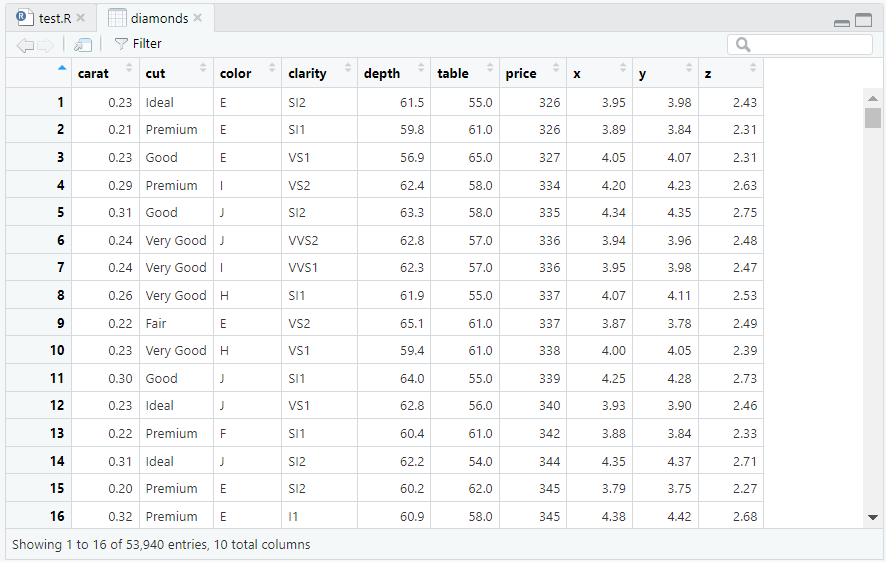
\includegraphics{fig/view1.png}

}

\caption{\label{fig-view1}打开 viewer 界面}

\end{figure}

\begin{figure}

{\centering 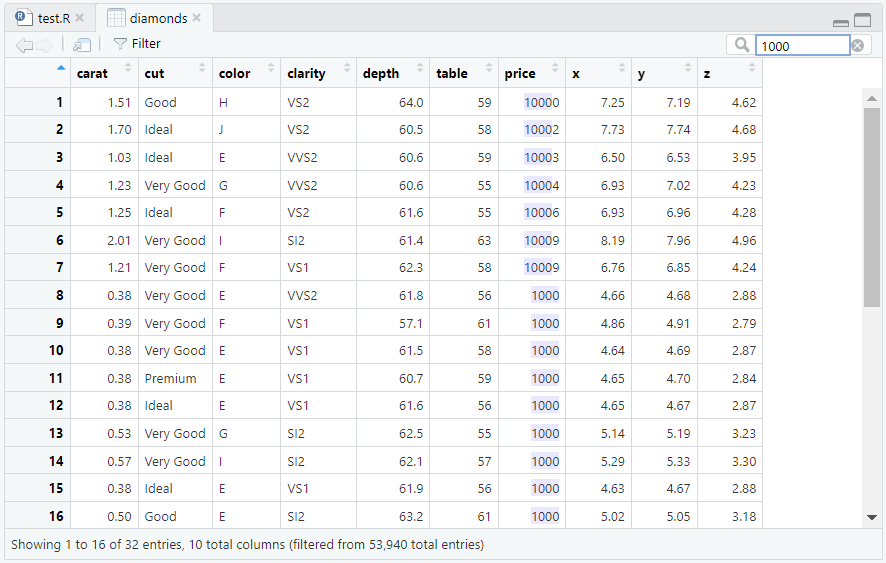
\includegraphics{fig/view2.png}

}

\caption{\label{fig-view2}搜索 ``1000''}

\end{figure}

\begin{figure}

{\centering 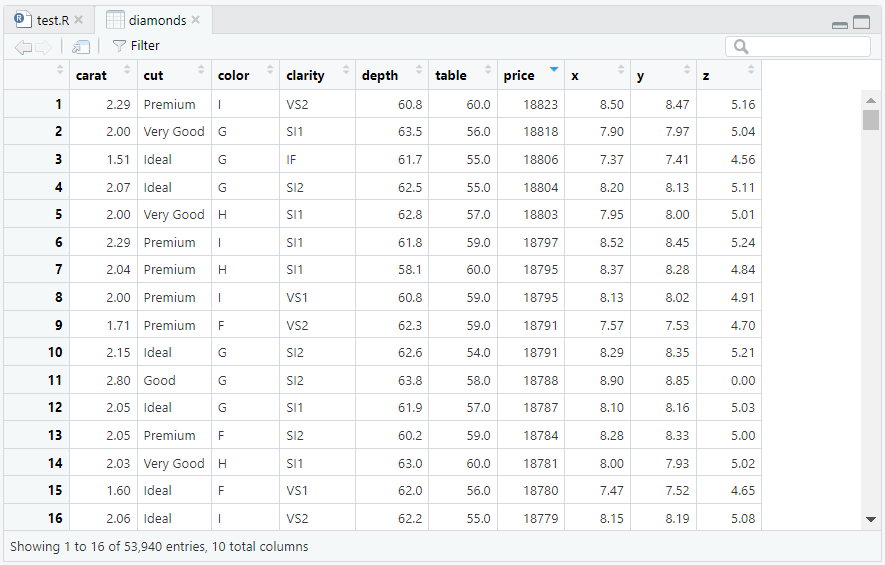
\includegraphics{fig/view3.png}

}

\caption{\label{fig-view3}根据 price 降序}

\end{figure}

\hypertarget{codebook}{%
\section{\texorpdfstring{\texttt{codebook()}}{codebook()}}\label{codebook}}

\begin{Shaded}
\begin{Highlighting}[]
\FunctionTok{library}\NormalTok{(statart)}

\CommentTok{\# 查看变量基本信息}
\FunctionTok{codebook}\NormalTok{(diamonds)}
\end{Highlighting}
\end{Shaded}

\begin{verbatim}
# A tibble: 10 x 4
   variable type        n unique
   <chr>    <chr>   <int>  <int>
 1 carat    double  53940    273
 2 cut      ordered 53940      5
 3 color    ordered 53940      7
 4 clarity  ordered 53940      8
 5 depth    double  53940    184
 6 table    double  53940    127
 7 price    integer 53940  11602
 8 x        double  53940    554
 9 y        double  53940    552
10 z        double  53940    375
\end{verbatim}

\hypertarget{dplyr-ux6392ux5e8f}{%
\chapter{dplyr 排序}\label{dplyr-ux6392ux5e8f}}

在 tidyverse 中,dplyr
是清理数据的最重要的包。下面,我将从最简单的排序函数开始介绍。

我们通常需要手动排序变量。而在排序个案时,因为变量具有算术性,所以我们可以根据某个(或某些)变量的取值,对个案进行快速排序。

\begin{itemize}
\tightlist
\item
  排序列(变量)

  \begin{itemize}
  \tightlist
  \item
    \texttt{relocate()} 把变量{\textbf{手动}}挪到开头

    \begin{itemize}
    \tightlist
    \item
      \texttt{.before} 和 \texttt{.after}
      {\textbf{精确地}}把变量挪到某个位置
    \end{itemize}
  \end{itemize}
\item
  排序行(个案)

  \begin{itemize}
  \tightlist
  \item
    \texttt{arrange()} 根据{\textbf{变量取值}}排序个案
  \end{itemize}
\end{itemize}

\hypertarget{relocate}{%
\section{\texorpdfstring{\texttt{relocate()}}{relocate()}}\label{relocate}}

让我们回到前面摘出来的示例数据。

\begin{Shaded}
\begin{Highlighting}[]
\FunctionTok{library}\NormalTok{(tidyverse)}

\NormalTok{diamonds }\CommentTok{\# 示例数据}
\end{Highlighting}
\end{Shaded}

\begin{verbatim}
# A tibble: 53,940 x 10
   carat cut       color clarity depth table price     x     y     z
   <dbl> <ord>     <ord> <ord>   <dbl> <dbl> <int> <dbl> <dbl> <dbl>
 1  0.23 Ideal     E     SI2      61.5    55   326  3.95  3.98  2.43
 2  0.21 Premium   E     SI1      59.8    61   326  3.89  3.84  2.31
 3  0.23 Good      E     VS1      56.9    65   327  4.05  4.07  2.31
 4  0.29 Premium   I     VS2      62.4    58   334  4.2   4.23  2.63
 5  0.31 Good      J     SI2      63.3    58   335  4.34  4.35  2.75
 6  0.24 Very Good J     VVS2     62.8    57   336  3.94  3.96  2.48
 7  0.24 Very Good I     VVS1     62.3    57   336  3.95  3.98  2.47
 8  0.26 Very Good H     SI1      61.9    55   337  4.07  4.11  2.53
 9  0.22 Fair      E     VS2      65.1    61   337  3.87  3.78  2.49
10  0.23 Very Good H     VS1      59.4    61   338  4     4.05  2.39
# i 53,930 more rows
\end{verbatim}

接下来,我将运行一些 \texttt{relocate()}
函数的示例,请特别关注列的顺序变化。

\begin{Shaded}
\begin{Highlighting}[]
\FunctionTok{relocate}\NormalTok{(diamonds, price) }\CommentTok{\# 把price变量提到最前,其余顺序不变}
\end{Highlighting}
\end{Shaded}

\begin{verbatim}
# A tibble: 53,940 x 10
   price carat cut       color clarity depth table     x     y     z
   <int> <dbl> <ord>     <ord> <ord>   <dbl> <dbl> <dbl> <dbl> <dbl>
 1   326  0.23 Ideal     E     SI2      61.5    55  3.95  3.98  2.43
 2   326  0.21 Premium   E     SI1      59.8    61  3.89  3.84  2.31
 3   327  0.23 Good      E     VS1      56.9    65  4.05  4.07  2.31
 4   334  0.29 Premium   I     VS2      62.4    58  4.2   4.23  2.63
 5   335  0.31 Good      J     SI2      63.3    58  4.34  4.35  2.75
 6   336  0.24 Very Good J     VVS2     62.8    57  3.94  3.96  2.48
 7   336  0.24 Very Good I     VVS1     62.3    57  3.95  3.98  2.47
 8   337  0.26 Very Good H     SI1      61.9    55  4.07  4.11  2.53
 9   337  0.22 Fair      E     VS2      65.1    61  3.87  3.78  2.49
10   338  0.23 Very Good H     VS1      59.4    61  4     4.05  2.39
# i 53,930 more rows
\end{verbatim}

\hypertarget{before-ux548c-.after}{%
\section{\texorpdfstring{\texttt{.before} 和
\texttt{.after}}{.before 和 .after}}\label{before-ux548c-.after}}

\begin{Shaded}
\begin{Highlighting}[]
\FunctionTok{relocate}\NormalTok{(diamonds, price, }\AttributeTok{.before =}\NormalTok{ cut) }\CommentTok{\# 把price提到cut之前,其余顺序不变}
\end{Highlighting}
\end{Shaded}

\begin{verbatim}
# A tibble: 53,940 x 10
   carat price cut       color clarity depth table     x     y     z
   <dbl> <int> <ord>     <ord> <ord>   <dbl> <dbl> <dbl> <dbl> <dbl>
 1  0.23   326 Ideal     E     SI2      61.5    55  3.95  3.98  2.43
 2  0.21   326 Premium   E     SI1      59.8    61  3.89  3.84  2.31
 3  0.23   327 Good      E     VS1      56.9    65  4.05  4.07  2.31
 4  0.29   334 Premium   I     VS2      62.4    58  4.2   4.23  2.63
 5  0.31   335 Good      J     SI2      63.3    58  4.34  4.35  2.75
 6  0.24   336 Very Good J     VVS2     62.8    57  3.94  3.96  2.48
 7  0.24   336 Very Good I     VVS1     62.3    57  3.95  3.98  2.47
 8  0.26   337 Very Good H     SI1      61.9    55  4.07  4.11  2.53
 9  0.22   337 Fair      E     VS2      65.1    61  3.87  3.78  2.49
10  0.23   338 Very Good H     VS1      59.4    61  4     4.05  2.39
# i 53,930 more rows
\end{verbatim}

\begin{Shaded}
\begin{Highlighting}[]
\FunctionTok{relocate}\NormalTok{(diamonds, price, }\AttributeTok{.after =}\NormalTok{ cut) }\CommentTok{\# 把price提到cut之后,其余顺序不变}
\end{Highlighting}
\end{Shaded}

\begin{verbatim}
# A tibble: 53,940 x 10
   carat cut       price color clarity depth table     x     y     z
   <dbl> <ord>     <int> <ord> <ord>   <dbl> <dbl> <dbl> <dbl> <dbl>
 1  0.23 Ideal       326 E     SI2      61.5    55  3.95  3.98  2.43
 2  0.21 Premium     326 E     SI1      59.8    61  3.89  3.84  2.31
 3  0.23 Good        327 E     VS1      56.9    65  4.05  4.07  2.31
 4  0.29 Premium     334 I     VS2      62.4    58  4.2   4.23  2.63
 5  0.31 Good        335 J     SI2      63.3    58  4.34  4.35  2.75
 6  0.24 Very Good   336 J     VVS2     62.8    57  3.94  3.96  2.48
 7  0.24 Very Good   336 I     VVS1     62.3    57  3.95  3.98  2.47
 8  0.26 Very Good   337 H     SI1      61.9    55  4.07  4.11  2.53
 9  0.22 Fair        337 E     VS2      65.1    61  3.87  3.78  2.49
10  0.23 Very Good   338 H     VS1      59.4    61  4     4.05  2.39
# i 53,930 more rows
\end{verbatim}

\hypertarget{arrange}{%
\section{\texorpdfstring{\texttt{arrange()}}{arrange()}}\label{arrange}}

在整洁数据中,对个案排序需要借助变量。

\begin{itemize}
\tightlist
\item
  在小学里,根据学号{\emph{(变量)}}排序,变的是小学生{\emph{(个案)}}的顺序。
\item
  在网购时,根据商品价格{\emph{(变量)}}排序,变的是商品{\emph{(个案)}}的顺序。
\item
  在12306买票时,根据列车发车时间{\emph{(变量)}}排序,变的是列车{\emph{(个案)}}的顺序。
\end{itemize}

\begin{tcolorbox}[enhanced jigsaw, bottomtitle=1mm, bottomrule=.15mm, coltitle=black, title=\textcolor{quarto-callout-important-color}{\faExclamation}\hspace{0.5em}{重要}, toptitle=1mm, colframe=quarto-callout-important-color-frame, colbacktitle=quarto-callout-important-color!10!white, opacitybacktitle=0.6, arc=.35mm, opacityback=0, breakable, toprule=.15mm, left=2mm, titlerule=0mm, rightrule=.15mm, colback=white, leftrule=.75mm]

变量的每个值都是一条个案,所以对单个变量排序的本质是改变个案顺序!

\end{tcolorbox}

这里我们借助了变量的统计能力(算术性)。反过来说,因为个案不具备统计能力,所以我们无法对变量做类似的排序,只能手动调整它们的位置。

\begin{Shaded}
\begin{Highlighting}[]
\FunctionTok{arrange}\NormalTok{(diamonds, price) }\CommentTok{\# 根据price变量升序(从低到高)}
\end{Highlighting}
\end{Shaded}

\begin{verbatim}
# A tibble: 53,940 x 10
   carat cut       color clarity depth table price     x     y     z
   <dbl> <ord>     <ord> <ord>   <dbl> <dbl> <int> <dbl> <dbl> <dbl>
 1  0.23 Ideal     E     SI2      61.5    55   326  3.95  3.98  2.43
 2  0.21 Premium   E     SI1      59.8    61   326  3.89  3.84  2.31
 3  0.23 Good      E     VS1      56.9    65   327  4.05  4.07  2.31
 4  0.29 Premium   I     VS2      62.4    58   334  4.2   4.23  2.63
 5  0.31 Good      J     SI2      63.3    58   335  4.34  4.35  2.75
 6  0.24 Very Good J     VVS2     62.8    57   336  3.94  3.96  2.48
 7  0.24 Very Good I     VVS1     62.3    57   336  3.95  3.98  2.47
 8  0.26 Very Good H     SI1      61.9    55   337  4.07  4.11  2.53
 9  0.22 Fair      E     VS2      65.1    61   337  3.87  3.78  2.49
10  0.23 Very Good H     VS1      59.4    61   338  4     4.05  2.39
# i 53,930 more rows
\end{verbatim}

\begin{Shaded}
\begin{Highlighting}[]
\FunctionTok{arrange}\NormalTok{(diamonds, }\SpecialCharTok{{-}}\NormalTok{price) }\CommentTok{\# 根据price变量降序(从高到低)}
\end{Highlighting}
\end{Shaded}

\begin{verbatim}
# A tibble: 53,940 x 10
   carat cut       color clarity depth table price     x     y     z
   <dbl> <ord>     <ord> <ord>   <dbl> <dbl> <int> <dbl> <dbl> <dbl>
 1  2.29 Premium   I     VS2      60.8    60 18823  8.5   8.47  5.16
 2  2    Very Good G     SI1      63.5    56 18818  7.9   7.97  5.04
 3  1.51 Ideal     G     IF       61.7    55 18806  7.37  7.41  4.56
 4  2.07 Ideal     G     SI2      62.5    55 18804  8.2   8.13  5.11
 5  2    Very Good H     SI1      62.8    57 18803  7.95  8     5.01
 6  2.29 Premium   I     SI1      61.8    59 18797  8.52  8.45  5.24
 7  2.04 Premium   H     SI1      58.1    60 18795  8.37  8.28  4.84
 8  2    Premium   I     VS1      60.8    59 18795  8.13  8.02  4.91
 9  1.71 Premium   F     VS2      62.3    59 18791  7.57  7.53  4.7 
10  2.15 Ideal     G     SI2      62.6    54 18791  8.29  8.35  5.21
# i 53,930 more rows
\end{verbatim}

\hypertarget{magrittr-ux7ba1ux9053}{%
\chapter{magrittr 管道}\label{magrittr-ux7ba1ux9053}}

\hypertarget{ux5b9aux4e49}{%
\section{\texorpdfstring{\texttt{\%\textgreater{}\%}
定义}{\%\textgreater\% 定义}}\label{ux5b9aux4e49}}

在继续讲解 dplyr 函数前,我想介绍一个非常特殊的函数,来自 magrittr
包的管道(pipe)函数 \texttt{\%\textgreater{}\%}。
它的用途是连通函数,美化代码。

它的定义如下

\begin{itemize}
\tightlist
\item
  \texttt{f(a)} 等于 \texttt{a\ \%\textgreater{}\%\ f()}
\item
  \texttt{f(a,\ b)} 等于 \texttt{a\ \%\textgreater{}\%\ f(b)}
\item
  \texttt{f(a,\ b,\ c,\ ...)} 等于
  \texttt{a\ \%\textgreater{}\%\ f(b,\ c,\ ...)}
\end{itemize}

比方说,\texttt{names(diamonds)} 等于
\texttt{diamonds\ \%\textgreater{}\%\ names()}。

\begin{tcolorbox}[enhanced jigsaw, bottomtitle=1mm, bottomrule=.15mm, coltitle=black, title=\textcolor{quarto-callout-warning-color}{\faExclamationTriangle}\hspace{0.5em}{警告}, toptitle=1mm, colframe=quarto-callout-warning-color-frame, colbacktitle=quarto-callout-warning-color!10!white, opacitybacktitle=0.6, arc=.35mm, opacityback=0, breakable, toprule=.15mm, left=2mm, titlerule=0mm, rightrule=.15mm, colback=white, leftrule=.75mm]

从下一章开始,为了帮助大家养成习惯,我会把几乎所有的函数都写成管道
\texttt{\%\textgreater{}\%} 的形式。

\end{tcolorbox}

\hypertarget{ux4f18ux70b9}{%
\section{\texorpdfstring{\texttt{\%\textgreater{}\%}
优点}{\%\textgreater\% 优点}}\label{ux4f18ux70b9}}

为什么要多此一举呢?在数据分析中,我们通常要用到大量的函数,比如我们要对一头牛做复杂的处理:

\textbf{【错误】写法一}

\begin{Shaded}
\begin{Highlighting}[]
\NormalTok{吃(蘸(涮(挤(捶打(切(宰(牛))), 成丸), 牛骨清汤), 沙茶))}
\end{Highlighting}
\end{Shaded}

\textbf{【错误】写法二}

\begin{Shaded}
\begin{Highlighting}[]
\NormalTok{吃(}
\NormalTok{  蘸(}
\NormalTok{    涮(}
\NormalTok{      挤(}
\NormalTok{        捶打(}
\NormalTok{          切(}
\NormalTok{            宰(牛)}
\NormalTok{          )}
\NormalTok{        ), 成丸}
\NormalTok{      ), 牛骨清汤}
\NormalTok{    ), 沙茶}
\NormalTok{  )}
\NormalTok{)}
\end{Highlighting}
\end{Shaded}

\textbf{【正确】写法三(使用管道)}

\begin{Shaded}
\begin{Highlighting}[]
\NormalTok{牛 }\SpecialCharTok{\%\textgreater{}\%}
\NormalTok{  宰() }\SpecialCharTok{\%\textgreater{}\%}
\NormalTok{  切() }\SpecialCharTok{\%\textgreater{}\%}
\NormalTok{  捶打() }\SpecialCharTok{\%\textgreater{}\%}
\NormalTok{  挤(成丸) }\SpecialCharTok{\%\textgreater{}\%}
\NormalTok{  涮(牛骨清汤) }\SpecialCharTok{\%\textgreater{}\%}
\NormalTok{  蘸(沙茶) }\SpecialCharTok{\%\textgreater{}\%}
\NormalTok{  吃()}
\end{Highlighting}
\end{Shaded}

第三种写法,明显更自然,更清晰。原来这一系列函数,把牛变成了手打牛肉丸,下清汤锅,蘸沙茶酱,填了肚子------想必是在潮汕地区吃的。

\begin{tcolorbox}[enhanced jigsaw, bottomtitle=1mm, bottomrule=.15mm, coltitle=black, title=\textcolor{quarto-callout-tip-color}{\faLightbulb}\hspace{0.5em}{提示}, toptitle=1mm, colframe=quarto-callout-tip-color-frame, colbacktitle=quarto-callout-tip-color!10!white, opacitybacktitle=0.6, arc=.35mm, opacityback=0, breakable, toprule=.15mm, left=2mm, titlerule=0mm, rightrule=.15mm, colback=white, leftrule=.75mm]

当我们有连续多个函数连在一起的时候,\texttt{\%\textgreater{}\%}
能让代码更加整洁、易读。

\end{tcolorbox}

\hypertarget{ux8303ux4f8b}{%
\section{\texorpdfstring{\texttt{\%\textgreater{}\%}
范例}{\%\textgreater\% 范例}}\label{ux8303ux4f8b}}

任务:先把 price 放到开头,再对它降序排列(从高到低)

\begin{Shaded}
\begin{Highlighting}[]
\CommentTok{\# 【错误】写法一}
\FunctionTok{arrange}\NormalTok{(}\FunctionTok{relocate}\NormalTok{(diamonds, price), }\SpecialCharTok{{-}}\NormalTok{price)}

\CommentTok{\# 【错误】写法二}
\FunctionTok{arrange}\NormalTok{(}
  \FunctionTok{relocate}\NormalTok{(diamonds, price),}
  \SpecialCharTok{{-}}\NormalTok{price}
\NormalTok{)}
\end{Highlighting}
\end{Shaded}

\begin{Shaded}
\begin{Highlighting}[]
\CommentTok{\# 【正确】写法三,整洁、清晰、易读}
\NormalTok{diamonds }\SpecialCharTok{\%\textgreater{}\%}
  \FunctionTok{relocate}\NormalTok{(price) }\SpecialCharTok{\%\textgreater{}\%}
  \FunctionTok{arrange}\NormalTok{(}\SpecialCharTok{{-}}\NormalTok{price)}
\end{Highlighting}
\end{Shaded}

\begin{verbatim}
# A tibble: 53,940 x 10
   price carat cut       color clarity depth table     x     y     z
   <int> <dbl> <ord>     <ord> <ord>   <dbl> <dbl> <dbl> <dbl> <dbl>
 1 18823  2.29 Premium   I     VS2      60.8    60  8.5   8.47  5.16
 2 18818  2    Very Good G     SI1      63.5    56  7.9   7.97  5.04
 3 18806  1.51 Ideal     G     IF       61.7    55  7.37  7.41  4.56
 4 18804  2.07 Ideal     G     SI2      62.5    55  8.2   8.13  5.11
 5 18803  2    Very Good H     SI1      62.8    57  7.95  8     5.01
 6 18797  2.29 Premium   I     SI1      61.8    59  8.52  8.45  5.24
 7 18795  2.04 Premium   H     SI1      58.1    60  8.37  8.28  4.84
 8 18795  2    Premium   I     VS1      60.8    59  8.13  8.02  4.91
 9 18791  1.71 Premium   F     VS2      62.3    59  7.57  7.53  4.7 
10 18791  2.15 Ideal     G     SI2      62.6    54  8.29  8.35  5.21
# i 53,930 more rows
\end{verbatim}

\hypertarget{ux548c}{%
\section{\texorpdfstring{\texttt{\%\textgreater{}\%} 和
\texttt{\textbar{}\textgreater{}}}{\%\textgreater\% 和 \textbar\textgreater{}}}\label{ux548c}}

在 R 4.1 的版本及以后,R 推出了所谓的自然管道(natural
pipe)\texttt{\textbar{}\textgreater{}}。它有三个优点,

\begin{enumerate}
\def\labelenumi{\arabic{enumi}.}
\tightlist
\item
  比较简洁,仅使用了两个字符;
\item
  和 Julia 等编程语言统一了语法;
\item
  随时可用,使用前不需要导入 tidyverse, dplyr 或 magnittr 包。
\end{enumerate}

鉴于上述优点,甚至 tidyverse 的奠基人 Hadley Wickham 都改用了
\texttt{\textbar{}\textgreater{}},几乎抛弃了
\texttt{\%\textgreater{}\%}。但是需要注意,\texttt{\textbar{}\textgreater{}}也有很多缺点,具体什么我就不赘述了,你们以后遇到了自然知道。

就我个人习惯而言,我还是用 \texttt{\%\textgreater{}\%}
更多一点。而且我也更推荐初学者用
\texttt{\%\textgreater{}\%},因为它更简单、更少报错。

\hypertarget{sec-wei}{%
\section{为所欲为}\label{sec-wei}}

我们已经学了一些 \texttt{dplyr} 函数。可以发现,几乎所有 \texttt{dplyr}
函数输入和输出的格式都是 tibble,这是一个非常精妙的设计。

\begin{figure}

\begin{minipage}[t]{0.50\linewidth}

{\centering 

\raisebox{-\height}{

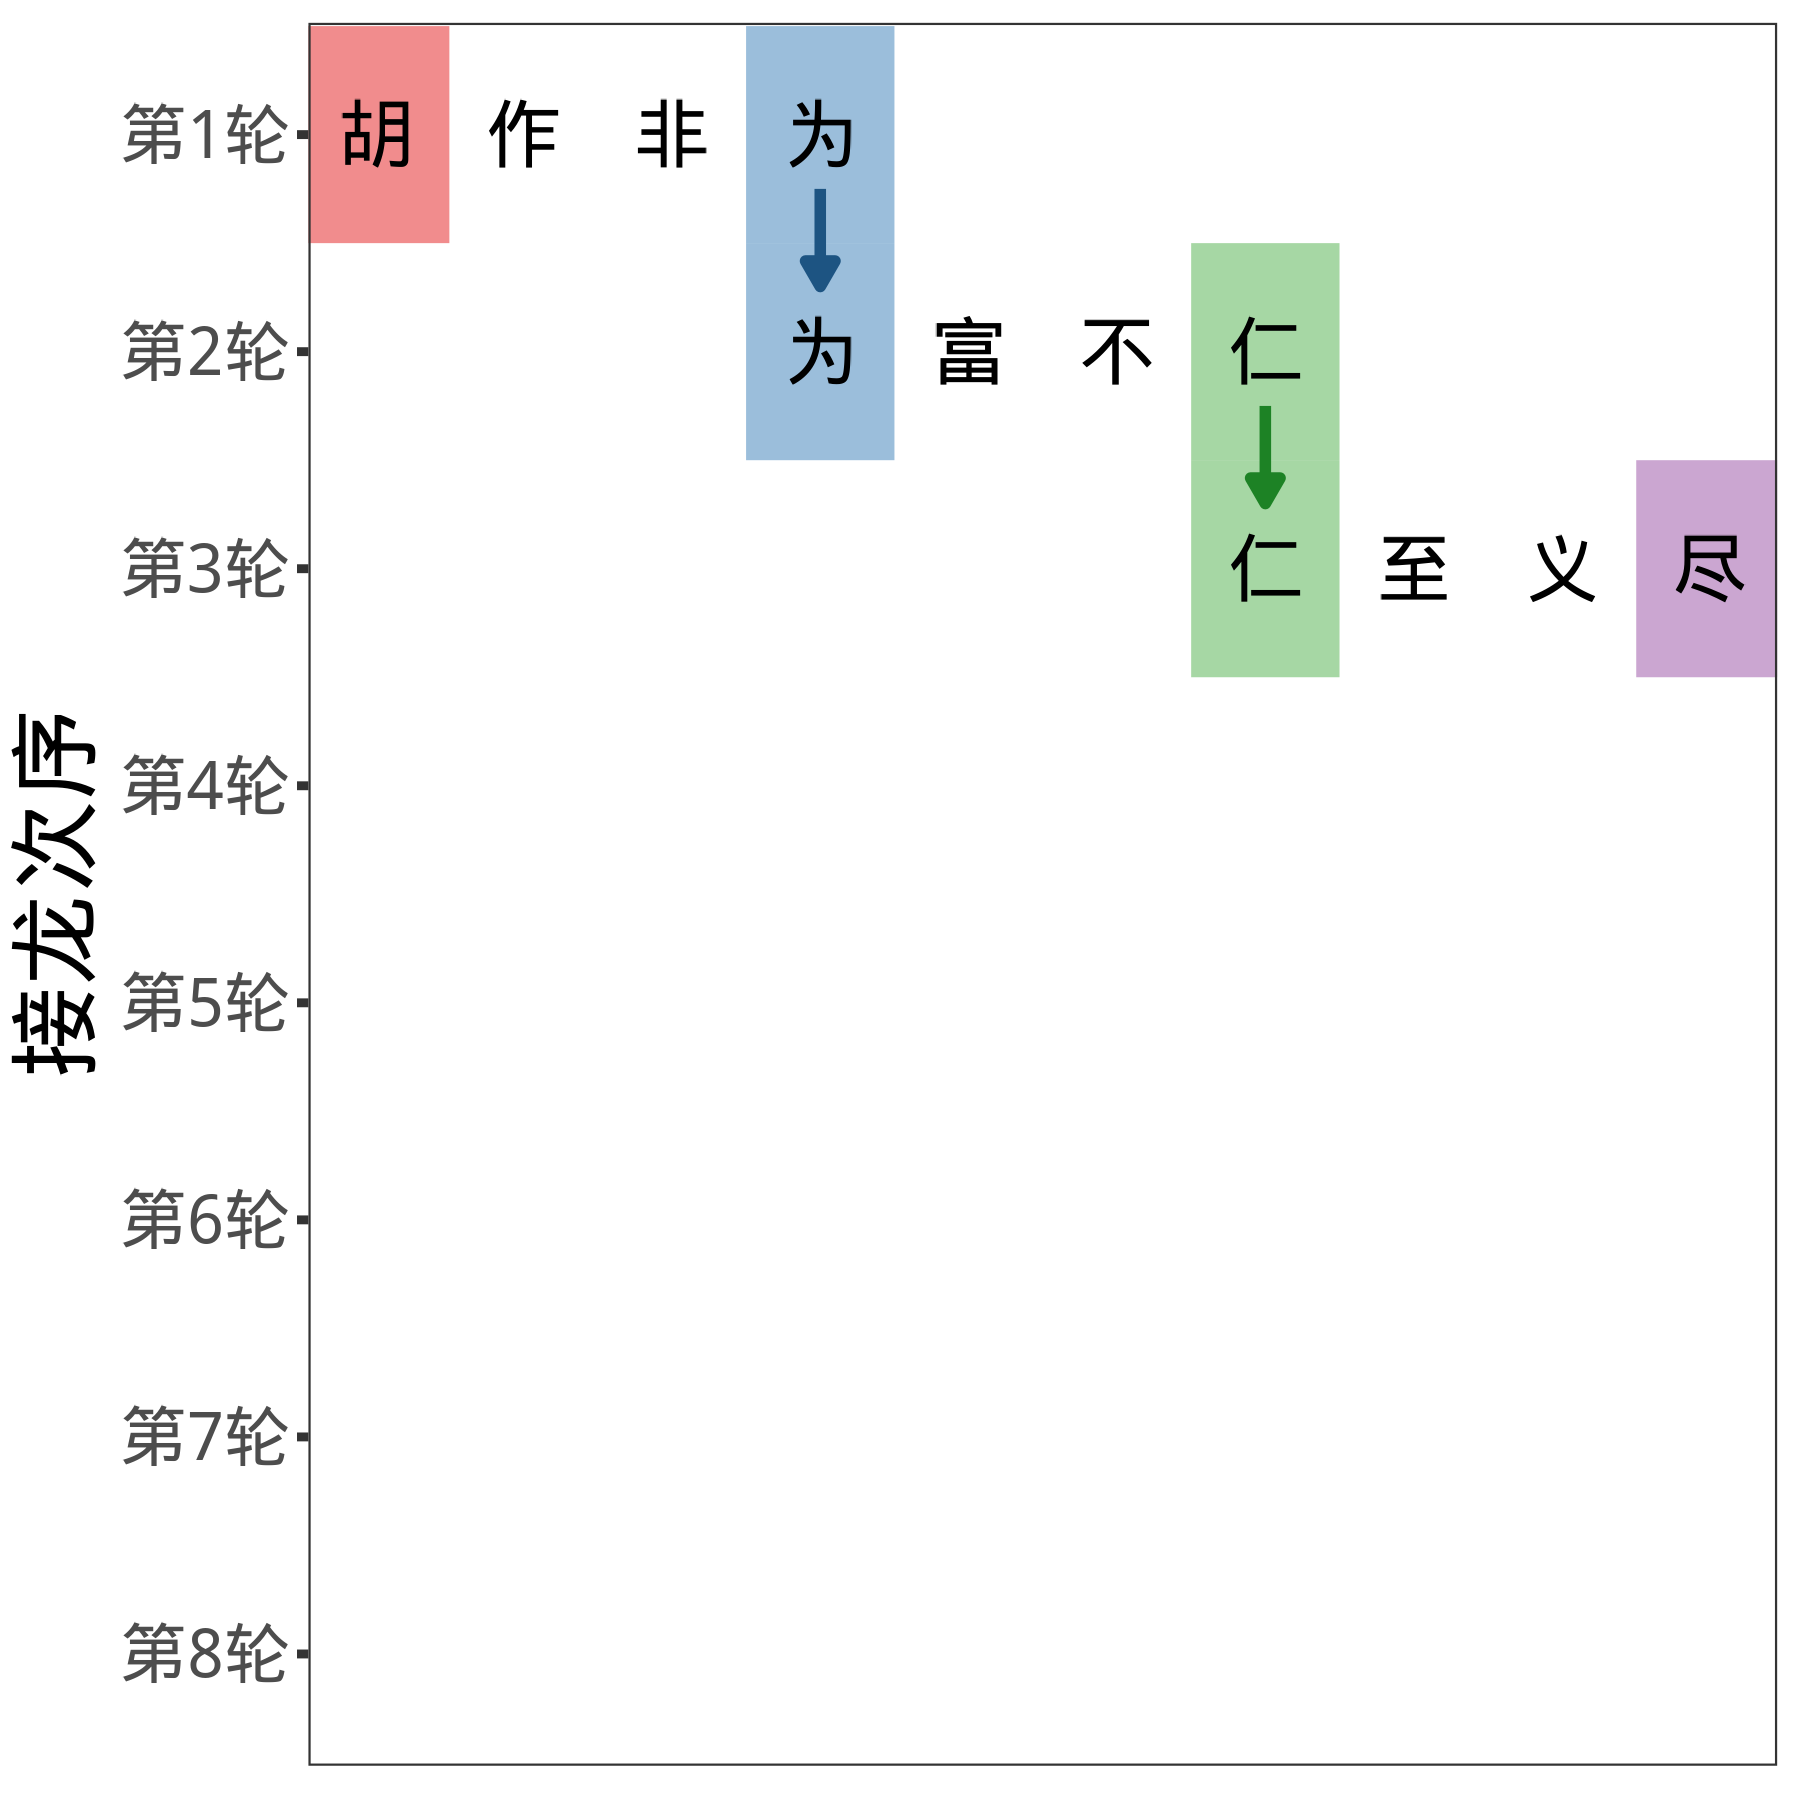
\includegraphics{fig/word_chain_short.png}

}

\caption{\label{fig-short}普通的成语接龙}

}

\end{minipage}%
%
\begin{minipage}[t]{0.50\linewidth}

{\centering 

\raisebox{-\height}{

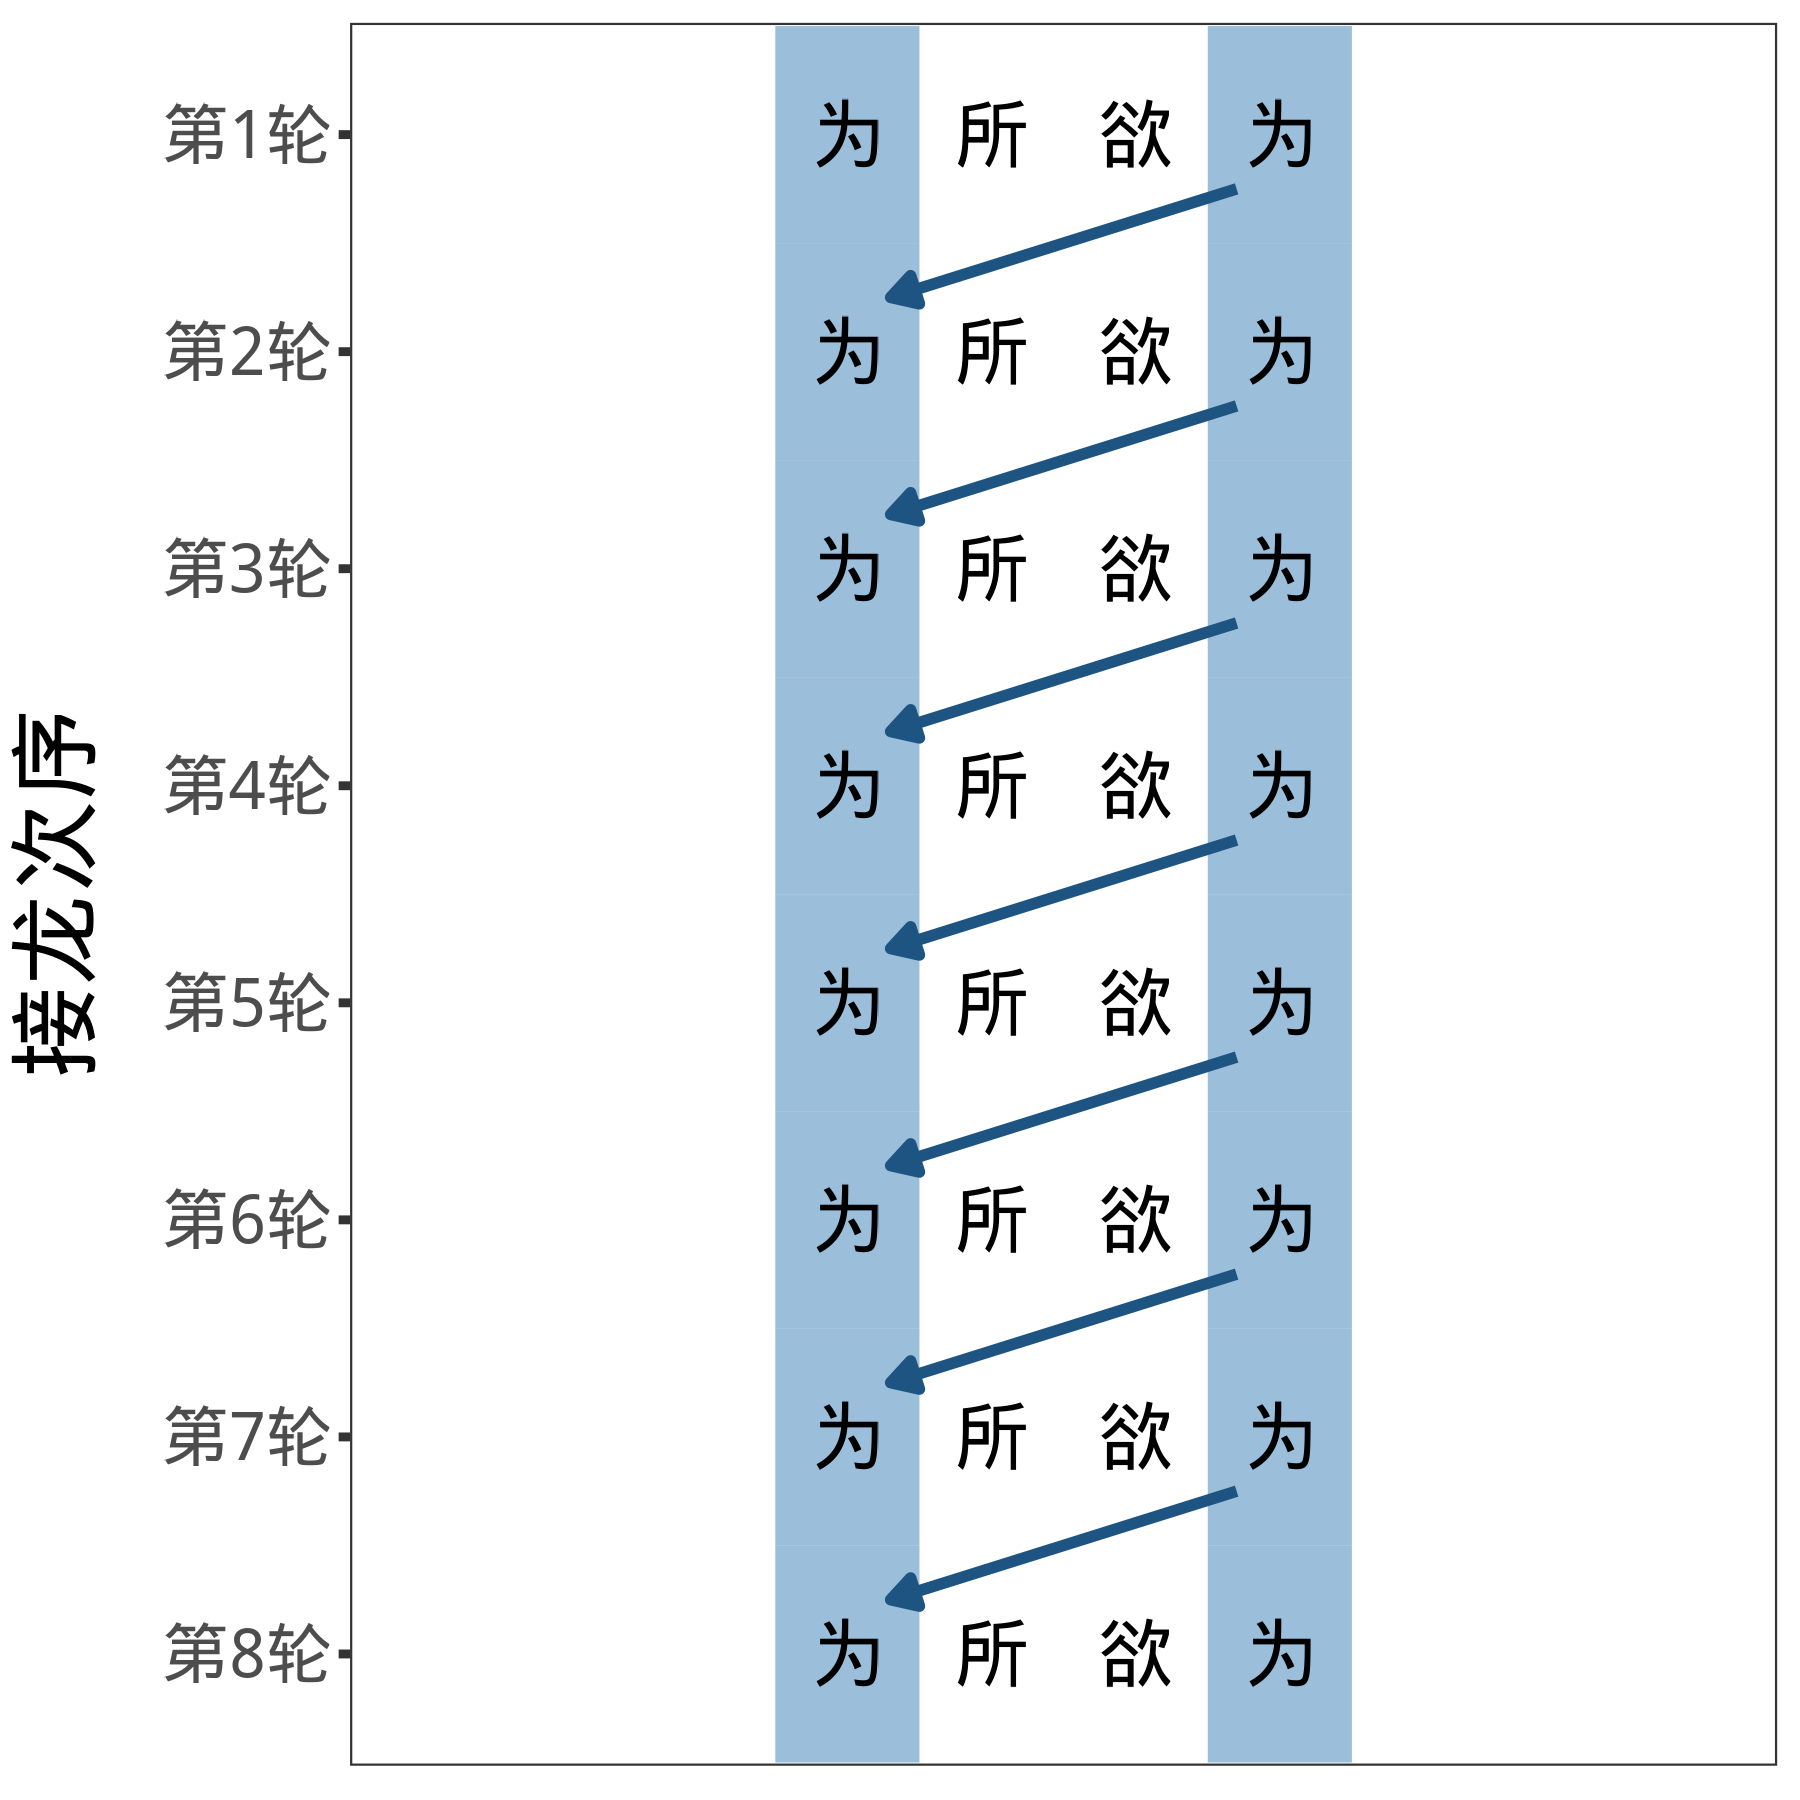
\includegraphics{fig/word_chain_long.png}

}

\caption{\label{fig-long}``为所欲为''的成语接龙}

}

\end{minipage}%

\end{figure}

章节~\ref{sec-chengyu}
说到,想要学会成语接龙,学``为所欲为''是最省时省力的。同理,

\begin{tcolorbox}[enhanced jigsaw, bottomtitle=1mm, bottomrule=.15mm, coltitle=black, title=\textcolor{quarto-callout-note-color}{\faInfo}\hspace{0.5em}{笔记}, toptitle=1mm, colframe=quarto-callout-note-color-frame, colbacktitle=quarto-callout-note-color!10!white, opacitybacktitle=0.6, arc=.35mm, opacityback=0, breakable, toprule=.15mm, left=2mm, titlerule=0mm, rightrule=.15mm, colback=white, leftrule=.75mm]

\begin{enumerate}
\def\labelenumi{\arabic{enumi}.}
\tightlist
\item
  使用 dplyr 函数,初学者可以``为所欲为''地处理 tibble。
\item
  dplyr 函数非常适配管道函数 \texttt{\%\textgreater{}\%}。
\end{enumerate}

\end{tcolorbox}

下面是一个简单的证明:

\begin{Shaded}
\begin{Highlighting}[]
\CommentTok{\# 定义识别函数}
\NormalTok{read\_object }\OtherTok{\textless{}{-}} \ControlFlowTok{function}\NormalTok{(object) \{}
\NormalTok{  input }\OtherTok{\textless{}{-}} \FunctionTok{substitute}\NormalTok{(object) }\SpecialCharTok{\%\textgreater{}\%}
    \FunctionTok{as.character}\NormalTok{()}
\NormalTok{  type }\OtherTok{\textless{}{-}} \FunctionTok{type\_sum}\NormalTok{(object) }\SpecialCharTok{\%\textgreater{}\%}
    \FunctionTok{as.character}\NormalTok{() }\SpecialCharTok{\%\textgreater{}\%}
    \FunctionTok{str\_extract}\NormalTok{(}\StringTok{"\^{}}\SpecialCharTok{\textbackslash{}\textbackslash{}}\StringTok{w+"}\NormalTok{)}

\NormalTok{  judgement }\OtherTok{\textless{}{-}} \FunctionTok{str\_glue}\NormalTok{(}
    \StringTok{"\{input\} 的类型是 \{type\}。"}
\NormalTok{  )}
  \FunctionTok{return}\NormalTok{(judgement)}
\NormalTok{\}}
\end{Highlighting}
\end{Shaded}

\begin{Shaded}
\begin{Highlighting}[]
\FunctionTok{read\_object}\NormalTok{(diamonds) }\CommentTok{\# 识别 diamonds}
\end{Highlighting}
\end{Shaded}

\begin{verbatim}
diamonds 的类型是 tibble。
\end{verbatim}

\begin{Shaded}
\begin{Highlighting}[]
\NormalTok{diamonds2 }\OtherTok{\textless{}{-}}\NormalTok{ diamonds }\SpecialCharTok{\%\textgreater{}\%}
  \FunctionTok{relocate}\NormalTok{(price)}

\FunctionTok{read\_object}\NormalTok{(diamonds2) }\CommentTok{\# 识别 diamonds2}
\end{Highlighting}
\end{Shaded}

\begin{verbatim}
diamonds2 的类型是 tibble。
\end{verbatim}

\begin{tcolorbox}[enhanced jigsaw, bottomtitle=1mm, bottomrule=.15mm, coltitle=black, title=\textcolor{quarto-callout-tip-color}{\faLightbulb}\hspace{0.5em}{提示}, toptitle=1mm, colframe=quarto-callout-tip-color-frame, colbacktitle=quarto-callout-tip-color!10!white, opacitybacktitle=0.6, arc=.35mm, opacityback=0, breakable, toprule=.15mm, left=2mm, titlerule=0mm, rightrule=.15mm, colback=white, leftrule=.75mm]

\texttt{relocate()} 输入 diamonds,输出 diamonds2,二者都是 tibble。

\end{tcolorbox}

\begin{Shaded}
\begin{Highlighting}[]
\NormalTok{diamonds3 }\OtherTok{\textless{}{-}}\NormalTok{ diamonds2 }\SpecialCharTok{\%\textgreater{}\%}
  \FunctionTok{arrange}\NormalTok{(}\SpecialCharTok{{-}}\NormalTok{price)}

\FunctionTok{read\_object}\NormalTok{(diamonds3) }\CommentTok{\# 识别 diamonds3}
\end{Highlighting}
\end{Shaded}

\begin{verbatim}
diamonds3 的类型是 tibble。
\end{verbatim}

\begin{tcolorbox}[enhanced jigsaw, bottomtitle=1mm, bottomrule=.15mm, coltitle=black, title=\textcolor{quarto-callout-tip-color}{\faLightbulb}\hspace{0.5em}{提示}, toptitle=1mm, colframe=quarto-callout-tip-color-frame, colbacktitle=quarto-callout-tip-color!10!white, opacitybacktitle=0.6, arc=.35mm, opacityback=0, breakable, toprule=.15mm, left=2mm, titlerule=0mm, rightrule=.15mm, colback=white, leftrule=.75mm]

同样,\texttt{arrange()} 输入 diamonds2,输出 diamonds3,二者都是
tibble。

\end{tcolorbox}

值得一提的是,tidyverse 底下的其他包,通常也有``为所欲为''的性质:

\begin{longtable}[]{@{}llll@{}}
\toprule\noalign{}
& 对象 & 函数 & 例子 \\
\midrule\noalign{}
\endhead
\bottomrule\noalign{}
\endlastfoot
成语接龙 & ``为'' & 特定成语 & ``为所欲为'' \\
数据 & tibble & dplyr 函数 & arrange(), relocate() 等 \\
图形 & gg & ggplot 函数 & geom\_col(), ggtitle() 等 \\
文本变量 & character & 部分 stringr 函数 & str\_replace(),
str\_extract() 等 \\
类别变量 & factor & 部分 forcats 函数 & fct\_reorder(), fct\_recode()
等 \\
列表 & list & 部分 purrr 函数 & map(), map2() 等 \\
\end{longtable}

\hypertarget{dplyr-ux9009ux53d6ux6216ux5220ux9664}{%
\chapter{dplyr 选取或删除}\label{dplyr-ux9009ux53d6ux6216ux5220ux9664}}

我删除了你的微信,本质上是保留了除了你以外所有人的微信。所以删除的本质就是选取。因此,在tidyverse里面,选取函数兼具了``保留''(选取)和``删除''的功能。

\begin{itemize}
\tightlist
\item
  列命令(选变量)

  \begin{itemize}
  \tightlist
  \item
    \texttt{select()} 根据{\textbf{位置}}或{\textbf{名称}}选取列

    \begin{itemize}
    \tightlist
    \item
      \texttt{:} 选取{\textbf{连续}}多个变量
    \item
      \texttt{c()} 选取{\textbf{任意}}多个变量
    \end{itemize}
  \item
    \texttt{select()} 根据{\textbf{变量取值}}选取列{(进阶技巧)}
  \item
    \texttt{pull()}
    根据位置或名称抽取一列,输出{\textbf{矢量}}格式{(进阶技巧)}
  \end{itemize}
\item
  行命令(选个案)

  \begin{itemize}
  \tightlist
  \item
    \texttt{head()} 和 \texttt{tail()}
    抽取数据的{\textbf{开头}}或{\textbf{结尾}}几行
  \item
    \texttt{slice()} 根据{\textbf{位置}}抽取行
  \item
    \texttt{filter()} 根据{\textbf{变量取值}}抽取行
  \item
    \texttt{slice\_sample} {\textbf{随机}}抽取若干行{(进阶技巧)}
  \item
    \texttt{distinct()} 去重,保留{\textbf{不重复}}的个案{(进阶技巧)}
  \end{itemize}
\end{itemize}

\hypertarget{select}{%
\section{\texorpdfstring{\texttt{select()}}{select()}}\label{select}}

\texttt{select()} 可以根据位置选取列。

\begin{Shaded}
\begin{Highlighting}[]
\FunctionTok{library}\NormalTok{(tidyverse)}
\NormalTok{diamonds }\SpecialCharTok{\%\textgreater{}\%}
  \FunctionTok{select}\NormalTok{(}\DecValTok{5}\NormalTok{) }\CommentTok{\# 抽取第五列}
\end{Highlighting}
\end{Shaded}

\begin{verbatim}
# A tibble: 53,940 x 1
   depth
   <dbl>
 1  61.5
 2  59.8
 3  56.9
 4  62.4
 5  63.3
 6  62.8
 7  62.3
 8  61.9
 9  65.1
10  59.4
# i 53,930 more rows
\end{verbatim}

\begin{Shaded}
\begin{Highlighting}[]
\NormalTok{diamonds }\SpecialCharTok{\%\textgreater{}\%}
  \FunctionTok{select}\NormalTok{(}\SpecialCharTok{{-}}\DecValTok{5}\NormalTok{) }\CommentTok{\# 删除第五列}
\end{Highlighting}
\end{Shaded}

\begin{verbatim}
# A tibble: 53,940 x 9
   carat cut       color clarity table price     x     y     z
   <dbl> <ord>     <ord> <ord>   <dbl> <int> <dbl> <dbl> <dbl>
 1  0.23 Ideal     E     SI2        55   326  3.95  3.98  2.43
 2  0.21 Premium   E     SI1        61   326  3.89  3.84  2.31
 3  0.23 Good      E     VS1        65   327  4.05  4.07  2.31
 4  0.29 Premium   I     VS2        58   334  4.2   4.23  2.63
 5  0.31 Good      J     SI2        58   335  4.34  4.35  2.75
 6  0.24 Very Good J     VVS2       57   336  3.94  3.96  2.48
 7  0.24 Very Good I     VVS1       57   336  3.95  3.98  2.47
 8  0.26 Very Good H     SI1        55   337  4.07  4.11  2.53
 9  0.22 Fair      E     VS2        61   337  3.87  3.78  2.49
10  0.23 Very Good H     VS1        61   338  4     4.05  2.39
# i 53,930 more rows
\end{verbatim}

\texttt{select()} 也可以根据名称选取列。

\begin{Shaded}
\begin{Highlighting}[]
\NormalTok{diamonds }\SpecialCharTok{\%\textgreater{}\%}
  \FunctionTok{select}\NormalTok{(cut) }\CommentTok{\# 选取cut变量}
\end{Highlighting}
\end{Shaded}

\begin{verbatim}
# A tibble: 53,940 x 1
   cut      
   <ord>    
 1 Ideal    
 2 Premium  
 3 Good     
 4 Premium  
 5 Good     
 6 Very Good
 7 Very Good
 8 Very Good
 9 Fair     
10 Very Good
# i 53,930 more rows
\end{verbatim}

\begin{Shaded}
\begin{Highlighting}[]
\NormalTok{diamonds }\SpecialCharTok{\%\textgreater{}\%}
  \FunctionTok{select}\NormalTok{(}\SpecialCharTok{{-}}\NormalTok{cut) }\CommentTok{\# 删除cut变量}
\end{Highlighting}
\end{Shaded}

\begin{verbatim}
# A tibble: 53,940 x 9
   carat color clarity depth table price     x     y     z
   <dbl> <ord> <ord>   <dbl> <dbl> <int> <dbl> <dbl> <dbl>
 1  0.23 E     SI2      61.5    55   326  3.95  3.98  2.43
 2  0.21 E     SI1      59.8    61   326  3.89  3.84  2.31
 3  0.23 E     VS1      56.9    65   327  4.05  4.07  2.31
 4  0.29 I     VS2      62.4    58   334  4.2   4.23  2.63
 5  0.31 J     SI2      63.3    58   335  4.34  4.35  2.75
 6  0.24 J     VVS2     62.8    57   336  3.94  3.96  2.48
 7  0.24 I     VVS1     62.3    57   336  3.95  3.98  2.47
 8  0.26 H     SI1      61.9    55   337  4.07  4.11  2.53
 9  0.22 E     VS2      65.1    61   337  3.87  3.78  2.49
10  0.23 H     VS1      59.4    61   338  4     4.05  2.39
# i 53,930 more rows
\end{verbatim}

\hypertarget{ux548c-c}{%
\section{\texorpdfstring{\texttt{:} 和
\texttt{c()}}{: 和 c()}}\label{ux548c-c}}

\texttt{:} 表示多个连续的整数。比如,

\begin{itemize}
\tightlist
\item
  \texttt{1:3} 表示 1\textasciitilde3 这三个整数
\item
  \texttt{-1:3} 表示 -1\textasciitilde3 这五个整数
\end{itemize}

\begin{Shaded}
\begin{Highlighting}[]
\DecValTok{1}\SpecialCharTok{:}\DecValTok{5}
\end{Highlighting}
\end{Shaded}

\begin{verbatim}
[1] 1 2 3 4 5
\end{verbatim}

\begin{Shaded}
\begin{Highlighting}[]
\CommentTok{\# 选取前五个变量}
\NormalTok{diamonds }\SpecialCharTok{\%\textgreater{}\%}
  \FunctionTok{select}\NormalTok{(}\DecValTok{1}\SpecialCharTok{:}\DecValTok{5}\NormalTok{)}
\end{Highlighting}
\end{Shaded}

\begin{verbatim}
# A tibble: 53,940 x 5
   carat cut       color clarity depth
   <dbl> <ord>     <ord> <ord>   <dbl>
 1  0.23 Ideal     E     SI2      61.5
 2  0.21 Premium   E     SI1      59.8
 3  0.23 Good      E     VS1      56.9
 4  0.29 Premium   I     VS2      62.4
 5  0.31 Good      J     SI2      63.3
 6  0.24 Very Good J     VVS2     62.8
 7  0.24 Very Good I     VVS1     62.3
 8  0.26 Very Good H     SI1      61.9
 9  0.22 Fair      E     VS2      65.1
10  0.23 Very Good H     VS1      59.4
# i 53,930 more rows
\end{verbatim}

\begin{Shaded}
\begin{Highlighting}[]
\CommentTok{\# 用另一种方式选取前五个变量}
\NormalTok{diamonds }\SpecialCharTok{\%\textgreater{}\%}
  \FunctionTok{select}\NormalTok{(carat}\SpecialCharTok{:}\NormalTok{depth)}
\end{Highlighting}
\end{Shaded}

\begin{verbatim}
# A tibble: 53,940 x 5
   carat cut       color clarity depth
   <dbl> <ord>     <ord> <ord>   <dbl>
 1  0.23 Ideal     E     SI2      61.5
 2  0.21 Premium   E     SI1      59.8
 3  0.23 Good      E     VS1      56.9
 4  0.29 Premium   I     VS2      62.4
 5  0.31 Good      J     SI2      63.3
 6  0.24 Very Good J     VVS2     62.8
 7  0.24 Very Good I     VVS1     62.3
 8  0.26 Very Good H     SI1      61.9
 9  0.22 Fair      E     VS2      65.1
10  0.23 Very Good H     VS1      59.4
# i 53,930 more rows
\end{verbatim}

\texttt{c()} 表示多个数的集合,它比 \texttt{:}
更灵活、更普适,缺点是写起来麻烦些。\texttt{c(1,\ 2,\ 3)} 和
\texttt{c(1:3)} 显然都不如 \texttt{1:3} 简洁。但是,\texttt{c()}
既可以表示不连续的整数,也可以表示其他类型的数:

\begin{itemize}
\tightlist
\item
  \texttt{c(1:3,\ 5)} 表示 1, 2, 3, 5 这四个数
\item
  \texttt{c(1:3,\ 5:6)} 表示 1, 2, 3, 5, 6 这五个数
\item
  \texttt{c(1.23,\ pi,\ exp(1),\ sqrt(2))} 表示 1.23, \(\pi\), \(e\),
  \(\sqrt{2}\) 这四个数

  \begin{itemize}
  \tightlist
  \item
    不过,只有整数能用来选变量哦
  \end{itemize}
\end{itemize}

\begin{Shaded}
\begin{Highlighting}[]
\FunctionTok{c}\NormalTok{(}\DecValTok{1}\NormalTok{, }\DecValTok{3}\SpecialCharTok{:}\DecValTok{5}\NormalTok{)}
\end{Highlighting}
\end{Shaded}

\begin{verbatim}
[1] 1 3 4 5
\end{verbatim}

\begin{Shaded}
\begin{Highlighting}[]
\CommentTok{\# 选取第1、3、4、5个变量}
\NormalTok{diamonds }\SpecialCharTok{\%\textgreater{}\%}
  \FunctionTok{select}\NormalTok{(}\FunctionTok{c}\NormalTok{(}\DecValTok{1}\NormalTok{, }\DecValTok{3}\SpecialCharTok{:}\DecValTok{5}\NormalTok{))}
\end{Highlighting}
\end{Shaded}

\begin{verbatim}
# A tibble: 53,940 x 4
   carat color clarity depth
   <dbl> <ord> <ord>   <dbl>
 1  0.23 E     SI2      61.5
 2  0.21 E     SI1      59.8
 3  0.23 E     VS1      56.9
 4  0.29 I     VS2      62.4
 5  0.31 J     SI2      63.3
 6  0.24 J     VVS2     62.8
 7  0.24 I     VVS1     62.3
 8  0.26 H     SI1      61.9
 9  0.22 E     VS2      65.1
10  0.23 H     VS1      59.4
# i 53,930 more rows
\end{verbatim}

\begin{Shaded}
\begin{Highlighting}[]
\CommentTok{\# 用另一种方式选取这些变量}
\NormalTok{diamonds }\SpecialCharTok{\%\textgreater{}\%}
  \FunctionTok{select}\NormalTok{(}\FunctionTok{c}\NormalTok{(carat, color}\SpecialCharTok{:}\NormalTok{depth))}
\end{Highlighting}
\end{Shaded}

\begin{verbatim}
# A tibble: 53,940 x 4
   carat color clarity depth
   <dbl> <ord> <ord>   <dbl>
 1  0.23 E     SI2      61.5
 2  0.21 E     SI1      59.8
 3  0.23 E     VS1      56.9
 4  0.29 I     VS2      62.4
 5  0.31 J     SI2      63.3
 6  0.24 J     VVS2     62.8
 7  0.24 I     VVS1     62.3
 8  0.26 H     SI1      61.9
 9  0.22 E     VS2      65.1
10  0.23 H     VS1      59.4
# i 53,930 more rows
\end{verbatim}

\hypertarget{head-ux548c-tail}{%
\section{\texorpdfstring{\texttt{head()} 和
\texttt{tail()}}{head() 和 tail()}}\label{head-ux548c-tail}}

\begin{Shaded}
\begin{Highlighting}[]
\NormalTok{diamonds }\SpecialCharTok{\%\textgreater{}\%}
  \FunctionTok{head}\NormalTok{() }\CommentTok{\# 抽取前六条}
\end{Highlighting}
\end{Shaded}

\begin{verbatim}
# A tibble: 6 x 10
  carat cut       color clarity depth table price     x     y     z
  <dbl> <ord>     <ord> <ord>   <dbl> <dbl> <int> <dbl> <dbl> <dbl>
1  0.23 Ideal     E     SI2      61.5    55   326  3.95  3.98  2.43
2  0.21 Premium   E     SI1      59.8    61   326  3.89  3.84  2.31
3  0.23 Good      E     VS1      56.9    65   327  4.05  4.07  2.31
4  0.29 Premium   I     VS2      62.4    58   334  4.2   4.23  2.63
5  0.31 Good      J     SI2      63.3    58   335  4.34  4.35  2.75
6  0.24 Very Good J     VVS2     62.8    57   336  3.94  3.96  2.48
\end{verbatim}

\begin{Shaded}
\begin{Highlighting}[]
\NormalTok{diamonds }\SpecialCharTok{\%\textgreater{}\%}
  \FunctionTok{tail}\NormalTok{() }\CommentTok{\# 抽取后六条}
\end{Highlighting}
\end{Shaded}

\begin{verbatim}
# A tibble: 6 x 10
  carat cut       color clarity depth table price     x     y     z
  <dbl> <ord>     <ord> <ord>   <dbl> <dbl> <int> <dbl> <dbl> <dbl>
1  0.72 Premium   D     SI1      62.7    59  2757  5.69  5.73  3.58
2  0.72 Ideal     D     SI1      60.8    57  2757  5.75  5.76  3.5 
3  0.72 Good      D     SI1      63.1    55  2757  5.69  5.75  3.61
4  0.7  Very Good D     SI1      62.8    60  2757  5.66  5.68  3.56
5  0.86 Premium   H     SI2      61      58  2757  6.15  6.12  3.74
6  0.75 Ideal     D     SI2      62.2    55  2757  5.83  5.87  3.64
\end{verbatim}

\hypertarget{slice}{%
\section{\texorpdfstring{\texttt{slice()}}{slice()}}\label{slice}}

比起 \texttt{head()} 和 \texttt{tail()},\texttt{slice()}
的语法要更复杂、更灵活一点。和 \texttt{select()} 类似,\texttt{slice()}
可以选取任意位置的若干行,再重新拼接起来,因此要列明所有行号。

\begin{Shaded}
\begin{Highlighting}[]
\NormalTok{diamonds }\SpecialCharTok{\%\textgreater{}\%}
  \FunctionTok{slice}\NormalTok{(}\DecValTok{5}\NormalTok{) }\CommentTok{\# 抽取第五条}
\end{Highlighting}
\end{Shaded}

\begin{verbatim}
# A tibble: 1 x 10
  carat cut   color clarity depth table price     x     y     z
  <dbl> <ord> <ord> <ord>   <dbl> <dbl> <int> <dbl> <dbl> <dbl>
1  0.31 Good  J     SI2      63.3    58   335  4.34  4.35  2.75
\end{verbatim}

\begin{Shaded}
\begin{Highlighting}[]
\NormalTok{diamonds }\SpecialCharTok{\%\textgreater{}\%}
  \FunctionTok{slice}\NormalTok{(}\DecValTok{1}\SpecialCharTok{:}\DecValTok{5}\NormalTok{) }\CommentTok{\# 抽取前五条}
\end{Highlighting}
\end{Shaded}

\begin{verbatim}
# A tibble: 5 x 10
  carat cut     color clarity depth table price     x     y     z
  <dbl> <ord>   <ord> <ord>   <dbl> <dbl> <int> <dbl> <dbl> <dbl>
1  0.23 Ideal   E     SI2      61.5    55   326  3.95  3.98  2.43
2  0.21 Premium E     SI1      59.8    61   326  3.89  3.84  2.31
3  0.23 Good    E     VS1      56.9    65   327  4.05  4.07  2.31
4  0.29 Premium I     VS2      62.4    58   334  4.2   4.23  2.63
5  0.31 Good    J     SI2      63.3    58   335  4.34  4.35  2.75
\end{verbatim}

\begin{Shaded}
\begin{Highlighting}[]
\NormalTok{diamonds }\SpecialCharTok{\%\textgreater{}\%}
  \FunctionTok{slice}\NormalTok{(}\SpecialCharTok{{-}}\DecValTok{5}\NormalTok{) }\CommentTok{\# 删除第五条}
\end{Highlighting}
\end{Shaded}

\begin{verbatim}
# A tibble: 53,939 x 10
   carat cut       color clarity depth table price     x     y     z
   <dbl> <ord>     <ord> <ord>   <dbl> <dbl> <int> <dbl> <dbl> <dbl>
 1  0.23 Ideal     E     SI2      61.5    55   326  3.95  3.98  2.43
 2  0.21 Premium   E     SI1      59.8    61   326  3.89  3.84  2.31
 3  0.23 Good      E     VS1      56.9    65   327  4.05  4.07  2.31
 4  0.29 Premium   I     VS2      62.4    58   334  4.2   4.23  2.63
 5  0.24 Very Good J     VVS2     62.8    57   336  3.94  3.96  2.48
 6  0.24 Very Good I     VVS1     62.3    57   336  3.95  3.98  2.47
 7  0.26 Very Good H     SI1      61.9    55   337  4.07  4.11  2.53
 8  0.22 Fair      E     VS2      65.1    61   337  3.87  3.78  2.49
 9  0.23 Very Good H     VS1      59.4    61   338  4     4.05  2.39
10  0.3  Good      J     SI1      64      55   339  4.25  4.28  2.73
# i 53,929 more rows
\end{verbatim}

\hypertarget{filter}{%
\section{\texorpdfstring{\texttt{filter()}}{filter()}}\label{filter}}

或许你还记得 \texttt{arrange()}
函数的讨论。我们说到变量具有统计能力,所以我们可以对单个变量排序,表现为改变个案顺序。同理,我们也可以对变量做判断,表现为筛选个案。

比方说,我们可以判断钻石的价格有没有低于 1000,且只保留那些 1000
以内的钻石。

\begin{Shaded}
\begin{Highlighting}[]
\NormalTok{diamonds }\SpecialCharTok{\%\textgreater{}\%}
  \FunctionTok{filter}\NormalTok{(price }\SpecialCharTok{\textless{}} \DecValTok{1000}\NormalTok{) }\CommentTok{\# 仅筛选$1000以内的钻石}
\end{Highlighting}
\end{Shaded}

\begin{verbatim}
# A tibble: 14,499 x 10
   carat cut       color clarity depth table price     x     y     z
   <dbl> <ord>     <ord> <ord>   <dbl> <dbl> <int> <dbl> <dbl> <dbl>
 1  0.23 Ideal     E     SI2      61.5    55   326  3.95  3.98  2.43
 2  0.21 Premium   E     SI1      59.8    61   326  3.89  3.84  2.31
 3  0.23 Good      E     VS1      56.9    65   327  4.05  4.07  2.31
 4  0.29 Premium   I     VS2      62.4    58   334  4.2   4.23  2.63
 5  0.31 Good      J     SI2      63.3    58   335  4.34  4.35  2.75
 6  0.24 Very Good J     VVS2     62.8    57   336  3.94  3.96  2.48
 7  0.24 Very Good I     VVS1     62.3    57   336  3.95  3.98  2.47
 8  0.26 Very Good H     SI1      61.9    55   337  4.07  4.11  2.53
 9  0.22 Fair      E     VS2      65.1    61   337  3.87  3.78  2.49
10  0.23 Very Good H     VS1      59.4    61   338  4     4.05  2.39
# i 14,489 more rows
\end{verbatim}

我们也可以判断钻石的净度是不是等于 VVS2,且只保留判断成立的钻石。

\begin{Shaded}
\begin{Highlighting}[]
\NormalTok{diamonds }\SpecialCharTok{\%\textgreater{}\%}
  \FunctionTok{filter}\NormalTok{(clarity }\SpecialCharTok{==} \StringTok{"VVS2"}\NormalTok{) }\CommentTok{\# 仅筛选VVS2级净度的钻石}
\end{Highlighting}
\end{Shaded}

\begin{verbatim}
# A tibble: 5,066 x 10
   carat cut       color clarity depth table price     x     y     z
   <dbl> <ord>     <ord> <ord>   <dbl> <dbl> <int> <dbl> <dbl> <dbl>
 1  0.24 Very Good J     VVS2     62.8    57   336  3.94  3.96  2.48
 2  0.23 Very Good G     VVS2     60.4    58   354  3.97  4.01  2.41
 3  0.28 Ideal     G     VVS2     61.4    56   553  4.19  4.22  2.58
 4  0.26 Very Good F     VVS2     59.2    60   554  4.19  4.22  2.49
 5  0.26 Very Good E     VVS2     59.9    58   554  4.15  4.23  2.51
 6  0.26 Very Good D     VVS2     62.4    54   554  4.08  4.13  2.56
 7  0.26 Very Good D     VVS2     62.8    60   554  4.01  4.05  2.53
 8  0.26 Ideal     E     VVS2     62.9    58   554  4.02  4.06  2.54
 9  0.24 Premium   H     VVS2     60.7    58   554  4.07  4.04  2.46
10  0.74 Ideal     I     VVS2     62.3    55  2761  5.77  5.81  3.61
# i 5,056 more rows
\end{verbatim}

\hypertarget{dplyr-ux66f4ux6539ux6216ux65b0ux5efa}{%
\chapter{dplyr 更改或新建}\label{dplyr-ux66f4ux6539ux6216ux65b0ux5efa}}

当你添加一个手机号到通讯录,手机会问你是``新建联系人''还是``添加到已有联系人''。这是两个不同的操作。不过,dplyr
的\texttt{mutate()}函数,将它们合二为一了。

\begin{itemize}
\tightlist
\item
  更改变量名

  \begin{itemize}
  \tightlist
  \item
    \texttt{rename()} 重命名
  \item
    \texttt{rename\_with()} 批量重命名{(进阶技巧)}
  \end{itemize}
\item
  更改或新建列(变量)

  \begin{itemize}
  \tightlist
  \item
    \texttt{mutate()} 更改、新建变量
  \item
    \texttt{fill()} 就近填充缺失值{(进阶技巧)}
  \item
    \texttt{replace\_na()} 批量替换缺失值{(进阶技巧)}
  \item
    \texttt{rownames\_to\_column()} 复制行名称为变量{(进阶技巧)}
  \item
    \texttt{add\_count()} 添加变量频数为新变量{(进阶技巧)}
  \item
    \texttt{unite()} 合并多个变量为一个{(进阶技巧)}
  \item
    \texttt{separate()等} 拆分一个变量为多个{(进阶技巧)}
  \item
    \texttt{add\_column()} \emph{手动添加变量}{(几乎不用)}
  \end{itemize}
\item
  更改或新建行(个案)

  \begin{itemize}
  \tightlist
  \item
    \texttt{expand()} 和 \texttt{complete()}
    根据变量取值的组合扩充个案{(进阶技巧)}
  \item
    \texttt{add\_row()} \emph{手动添加变量}{(几乎不用)}
  \end{itemize}
\end{itemize}

\hypertarget{rename}{%
\section{\texorpdfstring{\texttt{rename()}}{rename()}}\label{rename}}

\begin{Shaded}
\begin{Highlighting}[]
\FunctionTok{library}\NormalTok{(tidyverse)}

\CommentTok{\# 把 price 改名为 price\_usd}
\NormalTok{diamonds }\SpecialCharTok{\%\textgreater{}\%}
  \FunctionTok{rename}\NormalTok{(}\AttributeTok{price\_usd =}\NormalTok{ price)}
\end{Highlighting}
\end{Shaded}

\begin{verbatim}
# A tibble: 53,940 x 10
   carat cut       color clarity depth table price_usd     x     y     z
   <dbl> <ord>     <ord> <ord>   <dbl> <dbl>     <int> <dbl> <dbl> <dbl>
 1  0.23 Ideal     E     SI2      61.5    55       326  3.95  3.98  2.43
 2  0.21 Premium   E     SI1      59.8    61       326  3.89  3.84  2.31
 3  0.23 Good      E     VS1      56.9    65       327  4.05  4.07  2.31
 4  0.29 Premium   I     VS2      62.4    58       334  4.2   4.23  2.63
 5  0.31 Good      J     SI2      63.3    58       335  4.34  4.35  2.75
 6  0.24 Very Good J     VVS2     62.8    57       336  3.94  3.96  2.48
 7  0.24 Very Good I     VVS1     62.3    57       336  3.95  3.98  2.47
 8  0.26 Very Good H     SI1      61.9    55       337  4.07  4.11  2.53
 9  0.22 Fair      E     VS2      65.1    61       337  3.87  3.78  2.49
10  0.23 Very Good H     VS1      59.4    61       338  4     4.05  2.39
# i 53,930 more rows
\end{verbatim}

\begin{Shaded}
\begin{Highlighting}[]
\CommentTok{\# 把 x, y, z 分别改名为 size\_x, size\_y, size\_z}
\NormalTok{diamonds }\SpecialCharTok{\%\textgreater{}\%}
  \FunctionTok{rename}\NormalTok{(}
    \AttributeTok{size\_x =}\NormalTok{ x,}
    \AttributeTok{size\_y =}\NormalTok{ y,}
    \AttributeTok{size\_z =}\NormalTok{ z}
\NormalTok{  )}
\end{Highlighting}
\end{Shaded}

\begin{verbatim}
# A tibble: 53,940 x 10
   carat cut       color clarity depth table price size_x size_y size_z
   <dbl> <ord>     <ord> <ord>   <dbl> <dbl> <int>  <dbl>  <dbl>  <dbl>
 1  0.23 Ideal     E     SI2      61.5    55   326   3.95   3.98   2.43
 2  0.21 Premium   E     SI1      59.8    61   326   3.89   3.84   2.31
 3  0.23 Good      E     VS1      56.9    65   327   4.05   4.07   2.31
 4  0.29 Premium   I     VS2      62.4    58   334   4.2    4.23   2.63
 5  0.31 Good      J     SI2      63.3    58   335   4.34   4.35   2.75
 6  0.24 Very Good J     VVS2     62.8    57   336   3.94   3.96   2.48
 7  0.24 Very Good I     VVS1     62.3    57   336   3.95   3.98   2.47
 8  0.26 Very Good H     SI1      61.9    55   337   4.07   4.11   2.53
 9  0.22 Fair      E     VS2      65.1    61   337   3.87   3.78   2.49
10  0.23 Very Good H     VS1      59.4    61   338   4      4.05   2.39
# i 53,930 more rows
\end{verbatim}

\hypertarget{mutate}{%
\section{\texorpdfstring{\texttt{mutate()}}{mutate()}}\label{mutate}}

\begin{Shaded}
\begin{Highlighting}[]
\CommentTok{\# 新建变量 price\_rmb,即换算为人民币,假设汇率为7}
\NormalTok{diamonds }\SpecialCharTok{\%\textgreater{}\%}
  \FunctionTok{mutate}\NormalTok{(}\AttributeTok{price\_rmb =}\NormalTok{ price }\SpecialCharTok{*} \DecValTok{7}\NormalTok{)}
\end{Highlighting}
\end{Shaded}

\begin{verbatim}
# A tibble: 53,940 x 11
   carat cut       color clarity depth table price     x     y     z price_rmb
   <dbl> <ord>     <ord> <ord>   <dbl> <dbl> <int> <dbl> <dbl> <dbl>     <dbl>
 1  0.23 Ideal     E     SI2      61.5    55   326  3.95  3.98  2.43      2282
 2  0.21 Premium   E     SI1      59.8    61   326  3.89  3.84  2.31      2282
 3  0.23 Good      E     VS1      56.9    65   327  4.05  4.07  2.31      2289
 4  0.29 Premium   I     VS2      62.4    58   334  4.2   4.23  2.63      2338
 5  0.31 Good      J     SI2      63.3    58   335  4.34  4.35  2.75      2345
 6  0.24 Very Good J     VVS2     62.8    57   336  3.94  3.96  2.48      2352
 7  0.24 Very Good I     VVS1     62.3    57   336  3.95  3.98  2.47      2352
 8  0.26 Very Good H     SI1      61.9    55   337  4.07  4.11  2.53      2359
 9  0.22 Fair      E     VS2      65.1    61   337  3.87  3.78  2.49      2359
10  0.23 Very Good H     VS1      59.4    61   338  4     4.05  2.39      2366
# i 53,930 more rows
\end{verbatim}

\begin{Shaded}
\begin{Highlighting}[]
\CommentTok{\# 更改变量 price,换算为人民币,假设汇率为7}
\NormalTok{diamonds }\SpecialCharTok{\%\textgreater{}\%}
  \FunctionTok{mutate}\NormalTok{(}\AttributeTok{price =}\NormalTok{ price }\SpecialCharTok{*} \DecValTok{7}\NormalTok{)}
\end{Highlighting}
\end{Shaded}

\begin{verbatim}
# A tibble: 53,940 x 10
   carat cut       color clarity depth table price     x     y     z
   <dbl> <ord>     <ord> <ord>   <dbl> <dbl> <dbl> <dbl> <dbl> <dbl>
 1  0.23 Ideal     E     SI2      61.5    55  2282  3.95  3.98  2.43
 2  0.21 Premium   E     SI1      59.8    61  2282  3.89  3.84  2.31
 3  0.23 Good      E     VS1      56.9    65  2289  4.05  4.07  2.31
 4  0.29 Premium   I     VS2      62.4    58  2338  4.2   4.23  2.63
 5  0.31 Good      J     SI2      63.3    58  2345  4.34  4.35  2.75
 6  0.24 Very Good J     VVS2     62.8    57  2352  3.94  3.96  2.48
 7  0.24 Very Good I     VVS1     62.3    57  2352  3.95  3.98  2.47
 8  0.26 Very Good H     SI1      61.9    55  2359  4.07  4.11  2.53
 9  0.22 Fair      E     VS2      65.1    61  2359  3.87  3.78  2.49
10  0.23 Very Good H     VS1      59.4    61  2366  4     4.05  2.39
# i 53,930 more rows
\end{verbatim}

\begin{Shaded}
\begin{Highlighting}[]
\CommentTok{\# 新建变量 size,由 x, y, z 相乘而得(不代表钻石真实体积)}
\NormalTok{diamonds }\SpecialCharTok{\%\textgreater{}\%}
  \FunctionTok{mutate}\NormalTok{(}\AttributeTok{size =}\NormalTok{ x }\SpecialCharTok{*}\NormalTok{ y }\SpecialCharTok{*}\NormalTok{ z)}
\end{Highlighting}
\end{Shaded}

\begin{verbatim}
# A tibble: 53,940 x 11
   carat cut       color clarity depth table price     x     y     z  size
   <dbl> <ord>     <ord> <ord>   <dbl> <dbl> <int> <dbl> <dbl> <dbl> <dbl>
 1  0.23 Ideal     E     SI2      61.5    55   326  3.95  3.98  2.43  38.2
 2  0.21 Premium   E     SI1      59.8    61   326  3.89  3.84  2.31  34.5
 3  0.23 Good      E     VS1      56.9    65   327  4.05  4.07  2.31  38.1
 4  0.29 Premium   I     VS2      62.4    58   334  4.2   4.23  2.63  46.7
 5  0.31 Good      J     SI2      63.3    58   335  4.34  4.35  2.75  51.9
 6  0.24 Very Good J     VVS2     62.8    57   336  3.94  3.96  2.48  38.7
 7  0.24 Very Good I     VVS1     62.3    57   336  3.95  3.98  2.47  38.8
 8  0.26 Very Good H     SI1      61.9    55   337  4.07  4.11  2.53  42.3
 9  0.22 Fair      E     VS2      65.1    61   337  3.87  3.78  2.49  36.4
10  0.23 Very Good H     VS1      59.4    61   338  4     4.05  2.39  38.7
# i 53,930 more rows
\end{verbatim}

\hypertarget{dplyr-ux7edfux8ba1}{%
\chapter{dplyr 统计}\label{dplyr-ux7edfux8ba1}}

\begin{itemize}
\tightlist
\item
  类别变量

  \begin{itemize}
  \tightlist
  \item
    \texttt{count()} 计算各类别数量
  \item
    \texttt{tab()}
    计算各类别数量、{\textbf{百分比、累计百分比}}
  \item
    \texttt{tab1()} 同时列出{\textbf{多个}}变量的上述统计量
  \end{itemize}
\item
  连续变量

  \begin{itemize}
  \tightlist
  \item
    \texttt{summarise()} 统计{\textbf{个别}}统计量
  \item
    \texttt{summ()}
    快速生成{\textbf{大量}}变量的{\textbf{多个}}统计量
  \end{itemize}
\end{itemize}

\hypertarget{count}{%
\section{\texorpdfstring{\texttt{count()}}{count()}}\label{count}}

\begin{Shaded}
\begin{Highlighting}[]
\FunctionTok{library}\NormalTok{(tidyverse)}

\CommentTok{\# 显示每一类的数量}
\NormalTok{diamonds }\SpecialCharTok{\%\textgreater{}\%}
  \FunctionTok{count}\NormalTok{(cut)}
\end{Highlighting}
\end{Shaded}

\begin{verbatim}
# A tibble: 5 x 2
  cut           n
  <ord>     <int>
1 Fair       1610
2 Good       4906
3 Very Good 12082
4 Premium   13791
5 Ideal     21551
\end{verbatim}

\hypertarget{tab-ux548c-tab1}{%
\section{\texorpdfstring{\texttt{tab()} 和
\texttt{tab1()}}{tab() 和 tab1()}}\label{tab-ux548c-tab1}}

\begin{tcolorbox}[enhanced jigsaw, bottomtitle=1mm, bottomrule=.15mm, coltitle=black, title=\textcolor{quarto-callout-caution-color}{\faFire}\hspace{0.5em}{注意}, toptitle=1mm, colframe=quarto-callout-caution-color-frame, colbacktitle=quarto-callout-caution-color!10!white, opacitybacktitle=0.6, arc=.35mm, opacityback=0, breakable, toprule=.15mm, left=2mm, titlerule=0mm, rightrule=.15mm, colback=white, leftrule=.75mm]

这两个函数来自于我正在开发的 statart 包,暂时只能通过 \texttt{source()}
函数调用。

\end{tcolorbox}

\begin{Shaded}
\begin{Highlighting}[]
\CommentTok{\# 在 count() 的基础上,多了很多信息}
\NormalTok{diamonds }\SpecialCharTok{\%\textgreater{}\%}
  \FunctionTok{tab}\NormalTok{(cut)}
\end{Highlighting}
\end{Shaded}

\begin{verbatim}
# A tibble: 6 x 4
  cut           n percent    cum
  <chr>     <int>   <dbl>  <dbl>
1 Fair       1610    2.98   2.98
2 Good       4906    9.10  12.1 
3 Very Good 12082   22.4   34.5 
4 Premium   13791   25.6   60.0 
5 Ideal     21551   40.0  100   
6 total     53940  100     NA   
\end{verbatim}

\begin{Shaded}
\begin{Highlighting}[]
\CommentTok{\# 自动转换成列联表}
\NormalTok{diamonds }\SpecialCharTok{\%\textgreater{}\%}
  \FunctionTok{tab}\NormalTok{(cut, clarity)}
\end{Highlighting}
\end{Shaded}

\begin{verbatim}
# A tibble: 6 x 10
  cut          I1   SI2   SI1   VS2   VS1  VVS2  VVS1    IF total
  <chr>     <int> <int> <int> <int> <int> <int> <int> <int> <int>
1 Fair        210   466   408   261   170    69    17     9  1610
2 Good         96  1081  1560   978   648   286   186    71  4906
3 Very Good    84  2100  3240  2591  1775  1235   789   268 12082
4 Premium     205  2949  3575  3357  1989   870   616   230 13791
5 Ideal       146  2598  4282  5071  3589  2606  2047  1212 21551
6 total       741  9194 13065 12258  8171  5066  3655  1790 53940
\end{verbatim}

\begin{Shaded}
\begin{Highlighting}[]
\CommentTok{\# 同时 tab1() 多个变量}
\NormalTok{diamonds }\SpecialCharTok{\%\textgreater{}\%}
  \FunctionTok{tab1}\NormalTok{(cut}\SpecialCharTok{:}\NormalTok{clarity)}
\end{Highlighting}
\end{Shaded}

\begin{verbatim}
$cut
# A tibble: 6 x 4
  value         n percent    cum
  <chr>     <int>   <dbl>  <dbl>
1 Fair       1610    2.98   2.98
2 Good       4906    9.10  12.1 
3 Very Good 12082   22.4   34.5 
4 Premium   13791   25.6   60.0 
5 Ideal     21551   40.0  100   
6 total     53940  100     NA   

$color
# A tibble: 8 x 4
  value     n percent   cum
  <chr> <int>   <dbl> <dbl>
1 D      6775   12.6   12.6
2 E      9797   18.2   30.7
3 F      9542   17.7   48.4
4 G     11292   20.9   69.3
5 H      8304   15.4   84.7
6 I      5422   10.1   94.8
7 J      2808    5.21 100  
8 total 53940  100     NA  

$clarity
# A tibble: 9 x 4
  value     n percent    cum
  <chr> <int>   <dbl>  <dbl>
1 I1      741    1.37   1.37
2 SI2    9194   17.0   18.4 
3 SI1   13065   24.2   42.6 
4 VS2   12258   22.7   65.4 
5 VS1    8171   15.1   80.5 
6 VVS2   5066    9.39  89.9 
7 VVS1   3655    6.78  96.7 
8 IF     1790    3.32 100   
9 total 53940  100     NA   
\end{verbatim}

\begin{Shaded}
\begin{Highlighting}[]
\CommentTok{\# 同时 tab1() 多个变量,并返回成一个数据}
\NormalTok{diamonds }\SpecialCharTok{\%\textgreater{}\%}
  \FunctionTok{tab1}\NormalTok{(cut}\SpecialCharTok{:}\NormalTok{clarity, }\AttributeTok{.append =} \ConstantTok{TRUE}\NormalTok{)}
\end{Highlighting}
\end{Shaded}

\begin{verbatim}
# A tibble: 23 x 5
   variable value         n percent    cum
   <chr>    <chr>     <int>   <dbl>  <dbl>
 1 cut      Fair       1610    2.98   2.98
 2 cut      Good       4906    9.10  12.1 
 3 cut      Very Good 12082   22.4   34.5 
 4 cut      Premium   13791   25.6   60.0 
 5 cut      Ideal     21551   40.0  100   
 6 cut      total     53940  100     NA   
 7 color    D          6775   12.6   12.6 
 8 color    E          9797   18.2   30.7 
 9 color    F          9542   17.7   48.4 
10 color    G         11292   20.9   69.3 
11 color    H          8304   15.4   84.7 
12 color    I          5422   10.1   94.8 
13 color    J          2808    5.21 100   
14 color    total     53940  100     NA   
15 clarity  I1          741    1.37   1.37
16 clarity  SI2        9194   17.0   18.4 
17 clarity  SI1       13065   24.2   42.6 
18 clarity  VS2       12258   22.7   65.4 
19 clarity  VS1        8171   15.1   80.5 
20 clarity  VVS2       5066    9.39  89.9 
21 clarity  VVS1       3655    6.78  96.7 
22 clarity  IF         1790    3.32 100   
23 clarity  total     53940  100     NA   
\end{verbatim}

\hypertarget{summarise}{%
\section{\texorpdfstring{\texttt{summarise()}}{summarise()}}\label{summarise}}

\begin{Shaded}
\begin{Highlighting}[]
\CommentTok{\# 平均钻石价格}
\NormalTok{diamonds }\SpecialCharTok{\%\textgreater{}\%}
  \FunctionTok{summarise}\NormalTok{(}\FunctionTok{mean}\NormalTok{(price))}
\end{Highlighting}
\end{Shaded}

\begin{verbatim}
# A tibble: 1 x 1
  `mean(price)`
          <dbl>
1         3933.
\end{verbatim}

\begin{Shaded}
\begin{Highlighting}[]
\CommentTok{\# 指定变量名}
\NormalTok{diamonds }\SpecialCharTok{\%\textgreater{}\%}
  \FunctionTok{summarise}\NormalTok{(}\AttributeTok{price =} \FunctionTok{mean}\NormalTok{(price))}
\end{Highlighting}
\end{Shaded}

\begin{verbatim}
# A tibble: 1 x 1
  price
  <dbl>
1 3933.
\end{verbatim}

\hypertarget{summ}{%
\section{\texorpdfstring{\texttt{summ()}}{summ()}}\label{summ}}

为了解决 \texttt{summarise()}
太原始的问题,我尽可能兼顾简便和实用,设计了一个新的函数
\texttt{summ()}。下面我来演示一些基础功能:

\begin{tcolorbox}[enhanced jigsaw, bottomtitle=1mm, bottomrule=.15mm, coltitle=black, title=\textcolor{quarto-callout-caution-color}{\faFire}\hspace{0.5em}{注意}, toptitle=1mm, colframe=quarto-callout-caution-color-frame, colbacktitle=quarto-callout-caution-color!10!white, opacitybacktitle=0.6, arc=.35mm, opacityback=0, breakable, toprule=.15mm, left=2mm, titlerule=0mm, rightrule=.15mm, colback=white, leftrule=.75mm]

这个函数来自于我正在开发的 statart 包,暂时只能通过 \texttt{source()}
函数调用。

\end{tcolorbox}

\begin{Shaded}
\begin{Highlighting}[]
\CommentTok{\# 统计 price 的变量类型、非缺失数、类别数、均值、标准差、最小值和最大值}
\NormalTok{diamonds }\SpecialCharTok{\%\textgreater{}\%}
  \FunctionTok{summ}\NormalTok{(price)}
\end{Highlighting}
\end{Shaded}

\begin{verbatim}
# A tibble: 1 x 8
  variable type      n unique  mean    sd   min   max
  <chr>    <chr> <int>  <int> <dbl> <dbl> <int> <int>
1 price    int   53940  11602 3933. 3989.   326 18823
\end{verbatim}

解释一下上面的统计量:

\begin{itemize}
\tightlist
\item
  \texttt{variable} 是变量名
\item
  \texttt{type} 是变量类型(如变量有单位,则为单位)
\item
  \texttt{n} 是该变量非缺失值的数量
\item
  \texttt{unique} 是变量的类别数(有多少个不重复的取值)

  \begin{itemize}
  \tightlist
  \item
    显然,\texttt{unique} \(\leq\) \texttt{n}
  \item
    \texttt{unique} 越大,意味着这个变量越``连续'',信息越丰富
  \item
    比方说,\textbf{年龄}一般是0-120之间的某个正整数,而相应\textbf{月龄}的数量是年龄的12倍,\textbf{日龄}尤甚。所以在这三个变量里,\textbf{日龄}一般最平滑、最连续,信息量最大,相应的
    \texttt{unique} 数也最大。
  \end{itemize}
\item
  \texttt{mean} 是均值
\item
  \texttt{sd} 是标准差
\item
  \texttt{min} 是最小值
\item
  \texttt{max} 是最大值
\end{itemize}

\begin{Shaded}
\begin{Highlighting}[]
\CommentTok{\# 同时统计多个变量}
\NormalTok{diamonds }\SpecialCharTok{\%\textgreater{}\%}
  \FunctionTok{summ}\NormalTok{(x}\SpecialCharTok{:}\NormalTok{z)}
\end{Highlighting}
\end{Shaded}

\begin{verbatim}
# A tibble: 3 x 8
  variable type      n unique  mean    sd   min   max
  <chr>    <chr> <int>  <int> <dbl> <dbl> <dbl> <dbl>
1 x        dbl   53940    554  5.73 1.12      0  10.7
2 y        dbl   53940    552  5.73 1.14      0  58.9
3 z        dbl   53940    375  3.54 0.706     0  31.8
\end{verbatim}

在 x, y, z 这三个维度上,钻石的 z(高度)最小,而 x 和 y
的均值几乎一样。

\begin{Shaded}
\begin{Highlighting}[]
\CommentTok{\# 展示所有统计量}
\NormalTok{diamonds }\SpecialCharTok{\%\textgreater{}\%}
  \FunctionTok{summ}\NormalTok{(x}\SpecialCharTok{:}\NormalTok{z, }\AttributeTok{.detail =} \ConstantTok{TRUE}\NormalTok{) }\SpecialCharTok{\%\textgreater{}\%}
  \FunctionTok{print}\NormalTok{(}\AttributeTok{width =} \ConstantTok{Inf}\NormalTok{)}
\end{Highlighting}
\end{Shaded}

\begin{verbatim}
# A tibble: 3 x 18
  variable type      n unique miss_n valid_pct   min    q1 median  mean   mad
  <chr>    <chr> <int>  <int>  <int>     <dbl> <dbl> <dbl>  <dbl> <dbl> <dbl>
1 x        dbl   53940    554      0         1     0  4.71   5.7   5.73 1.38 
2 y        dbl   53940    552      0         1     0  4.72   5.71  5.73 1.36 
3 z        dbl   53940    375      0         1     0  2.91   3.53  3.54 0.845
     sd    q3   max   iqr  skew kurtosis      se
  <dbl> <dbl> <dbl> <dbl> <dbl>    <dbl>   <dbl>
1 1.12   6.54  10.7  1.83 0.379   -0.618 0.00483
2 1.14   6.54  58.9  1.82 2.43    91.2   0.00492
3 0.706  4.04  31.8  1.13 1.52    47.1   0.00304
\end{verbatim}

可以看到,其实 x 和 y 在四分位数(q1 和
q3)上没有什么差别,但是它们的最大值(max)、偏度(skew)和峰度(kurtosis)上相差很多。我猜想,对于一些不规则的钻石,可能会把短边选为
x,而长边选为 y。

\begin{Shaded}
\begin{Highlighting}[]
\CommentTok{\# 自己选择一些统计量}
\NormalTok{diamonds }\SpecialCharTok{\%\textgreater{}\%}
  \FunctionTok{summ}\NormalTok{(x}\SpecialCharTok{:}\NormalTok{z, }\AttributeTok{.stat =} \FunctionTok{c}\NormalTok{(}\StringTok{"valid\_pct"}\NormalTok{, }\StringTok{"mean"}\NormalTok{, }\StringTok{"se"}\NormalTok{))}
\end{Highlighting}
\end{Shaded}

\begin{verbatim}
# A tibble: 3 x 5
  variable type  valid_pct  mean      se
  <chr>    <chr>     <dbl> <dbl>   <dbl>
1 x        dbl           1  5.73 0.00483
2 y        dbl           1  5.73 0.00492
3 z        dbl           1  3.54 0.00304
\end{verbatim}

valid\_pct 表示非缺失值的比例,这里为1,说明完全无缺失。se
是标准误,也就是对均值的误差估计。

\begin{Shaded}
\begin{Highlighting}[]
\CommentTok{\# 一次性选择所有变量}
\NormalTok{diamonds }\SpecialCharTok{\%\textgreater{}\%}
  \FunctionTok{summ}\NormalTok{(}\FunctionTok{everything}\NormalTok{())}
\end{Highlighting}
\end{Shaded}

\begin{verbatim}
Warning in summ(., everything()): 
      cut, color, clarity are factor variables.
      They are summarised (***), but the statistics may be misleading.
      Consider using `tab1()` instead.
\end{verbatim}

\begin{verbatim}
# A tibble: 10 x 8
   variable   type      n unique     mean       sd   min      max
   <chr>      <chr> <int>  <int>    <dbl>    <dbl> <dbl>    <dbl>
 1 carat      dbl   53940    273    0.798    0.474   0.2     5.01
 2 cut***     ord   53940      5    3.90     1.12    1       5   
 3 color***   ord   53940      7    3.59     1.70    1       7   
 4 clarity*** ord   53940      8    4.05     1.65    1       8   
 5 depth      dbl   53940    184   61.7      1.43   43      79   
 6 table      dbl   53940    127   57.5      2.23   43      95   
 7 price      int   53940  11602 3933.    3989.    326   18823   
 8 x          dbl   53940    554    5.73     1.12    0      10.7 
 9 y          dbl   53940    552    5.73     1.14    0      58.9 
10 z          dbl   53940    375    3.54     0.706   0      31.8 
\end{verbatim}

请注意,因为 cut, color, clarity 都是定序变量,所以 \texttt{summ()}
它们比较牵强。对它们使用前文的 \texttt{tab1()} 会更为合适。

\begin{verbatim}
Rows: 1,000
Columns: 14
$ date      <date> 2024-02-08, 2024-02-07, 2024-02-06, 2024-02-05, 2024-02-04,~
$ time      <dttm> 2024-02-09 11:59:59, 2024-02-09 11:59:58, 2024-02-09 11:59:~
$ duration1 <drtn> 3 hours, 4 hours, 5 hours, 6 hours, 7 hours, 8 hours, 9 hou~
$ duration2 <time> 12:34:56, 12:34:56, 12:34:56, 12:34:56, 12:34:56, 12:34:56,~
$ string    <chr> "ABC", "ABC", "ABC", "ABC", "ABC", "ABC", "ABC", "ABC", "ABC~
$ logical   <lgl> TRUE, FALSE, TRUE, FALSE, TRUE, FALSE, TRUE, FALSE, TRUE, FA~
$ unit1     [m] 1 [m], 2 [m], 3 [m], 4 [m], 5 [m], 6 [m], 7 [m], 8 [m], 9 [m],~
$ unit2     [m^2] 1 [m^2], 2 [m^2], 3 [m^2], 4 [m^2], 5 [m^2], 6 [m^2], 7 [m^2~
$ factor    <fct> a, b, a, b, a, b, a, b, a, b, a, b, a, b, a, b, a, b, a, b, ~
$ order     <ord> a, b, a, b, a, b, a, b, a, b, a, b, a, b, a, b, a, b, a, b, ~
$ double    <dbl> 0.1, 0.2, 0.3, 0.4, 0.5, 0.6, 0.7, 0.8, 0.9, 1.0, 1.1, 1.2, ~
$ integer   <int> 1, 2, 3, 4, 5, 6, 7, 8, 9, 10, 11, 12, 13, 14, 15, 16, 17, 1~
$ half_miss <dbl> 1, NA, 3, NA, 5, NA, 7, NA, 9, NA, 11, NA, 13, NA, 15, NA, 1~
$ all_miss  <dbl> NA, NA, NA, NA, NA, NA, NA, NA, NA, NA, NA, NA, NA, NA, NA, ~
\end{verbatim}

\begin{Shaded}
\begin{Highlighting}[]
\NormalTok{complex\_tb }\SpecialCharTok{\%\textgreater{}\%}
  \FunctionTok{codebook}\NormalTok{()}
\end{Highlighting}
\end{Shaded}

\begin{verbatim}
Warning in un[i] <- at$units: number of items to replace is not a multiple of
replacement length

Warning in un[i] <- at$units: number of items to replace is not a multiple of
replacement length
\end{verbatim}

\begin{verbatim}
# A tibble: 14 x 4
   variable  type                 n unique
   <chr>     <chr>            <int>  <int>
 1 date      date              1000   1000
 2 time      datetime          1000   1000
 3 duration1 duration [hours]  1000   1000
 4 duration2 time [secs]       1000      1
 5 string    character         1000      1
 6 logical   logical           1000      2
 7 unit1     units [m]         1000   1000
 8 unit2     units [m^2]       1000   1000
 9 factor    factor            1000      2
10 order     ordered           1000      2
11 double    double            1000   1000
12 integer   integer           1000   1000
13 half_miss double             500    500
14 all_miss  double               0      0
\end{verbatim}

\begin{Shaded}
\begin{Highlighting}[]
\NormalTok{complex\_tb }\SpecialCharTok{\%\textgreater{}\%}
  \FunctionTok{summ}\NormalTok{(}\FunctionTok{everything}\NormalTok{())}
\end{Highlighting}
\end{Shaded}

\begin{verbatim}
Warning in summ(., everything()): 
    string is non-numeric.
    Use `tab()` instead.
\end{verbatim}

\begin{verbatim}
Warning in summ(., everything()): 
      date, time are date or datetime variables.
      Use `summ_date()` or `summ_all()` instead.
\end{verbatim}

\begin{verbatim}
Warning in summ(., everything()): 
      factor, order are factor variables.
      They are summarised (***), but the statistics may be misleading.
      Consider using `tab1()` instead.
\end{verbatim}

\begin{verbatim}
Warning in summ(., everything()): 
    all_miss is entirely missing and thus removed.
\end{verbatim}

\begin{verbatim}
# A tibble: 10 x 8
   variable  type        n unique    mean      sd     min   max
   <chr>     <chr>   <int>  <int>   <dbl>   <dbl>   <dbl> <dbl>
 1 duration1 [hours]  1000   1000   502.  289.        3    1002
 2 duration2 [secs]   1000      1 45296     0     45296   45296
 3 logical   lgl      1000      2     0.5   0.500     0       1
 4 unit1     [m]      1000   1000   500.  289.        1    1000
 5 unit2     [m^2]    1000   1000   500.  289.        1    1000
 6 factor*** fct      1000      2     1.5   0.500     1       2
 7 order***  ord      1000      2     1.5   0.500     1       2
 8 double    dbl      1000   1000    50.0  28.9       0.1   100
 9 integer   int      1000   1000   500.  289.        1    1000
10 half_miss dbl       500    500   500   289.        1     999
\end{verbatim}

\hypertarget{dplyr-ux5206ux7ec4}{%
\chapter{dplyr 分组}\label{dplyr-ux5206ux7ec4}}

分组可以做很多事情,但最常用的,肯定还是分组统计。

\begin{itemize}
\tightlist
\item
  \texttt{.by} 在函数中分组

  \begin{itemize}
  \tightlist
  \item
    \texttt{summarise(...,\ .by)} 统计{\textbf{个别}}统计量
  \item
    \texttt{summ(...,\ .by)}
    快速生成{\textbf{大量}}变量的{\textbf{多个}}统计量
  \item
    \texttt{mutate(...,\ .by)} 根据分组统计量更改或新建变量
  \end{itemize}
\item
  \texttt{group\_by()} 在函数前构造分组数据
\item
  \texttt{ungroup()} 取消数据分组
\end{itemize}

\hypertarget{summarise...-.by}{%
\section{\texorpdfstring{\texttt{summarise(...,\ .by)}}{summarise(..., .by)}}\label{summarise...-.by}}

\begin{Shaded}
\begin{Highlighting}[]
\FunctionTok{library}\NormalTok{(tidyverse)}
\end{Highlighting}
\end{Shaded}

\begin{verbatim}
Warning: package 'ggplot2' was built under R version 4.3.3
\end{verbatim}

\begin{verbatim}
Warning: package 'stringr' was built under R version 4.3.2
\end{verbatim}

\begin{verbatim}
-- Attaching core tidyverse packages ------------------------ tidyverse 2.0.0 --
v dplyr     1.1.2     v readr     2.1.4
v forcats   1.0.0     v stringr   1.5.1
v ggplot2   3.5.1     v tibble    3.2.1
v lubridate 1.9.2     v tidyr     1.3.0
v purrr     1.0.1     
-- Conflicts ------------------------------------------ tidyverse_conflicts() --
x dplyr::filter() masks stats::filter()
x dplyr::lag()    masks stats::lag()
i Use the conflicted package (<http://conflicted.r-lib.org/>) to force all conflicts to become errors
\end{verbatim}

\begin{Shaded}
\begin{Highlighting}[]
\NormalTok{diamonds }\SpecialCharTok{\%\textgreater{}\%}
  \FunctionTok{summarise}\NormalTok{(}
    \AttributeTok{price =} \FunctionTok{mean}\NormalTok{(price),}
    \AttributeTok{.by =}\NormalTok{ clarity}
\NormalTok{  )}
\end{Highlighting}
\end{Shaded}

\begin{verbatim}
# A tibble: 8 x 2
  clarity price
  <ord>   <dbl>
1 SI2     5063.
2 SI1     3996.
3 VS1     3839.
4 VS2     3925.
5 VVS2    3284.
6 VVS1    2523.
7 I1      3924.
8 IF      2865.
\end{verbatim}

\begin{Shaded}
\begin{Highlighting}[]
\NormalTok{diamonds }\SpecialCharTok{\%\textgreater{}\%}
  \FunctionTok{summarise}\NormalTok{(}
    \AttributeTok{price =} \FunctionTok{mean}\NormalTok{(price),}
    \AttributeTok{.by =} \FunctionTok{c}\NormalTok{(cut, clarity)}
\NormalTok{  )}
\end{Highlighting}
\end{Shaded}

\begin{verbatim}
# A tibble: 40 x 3
   cut       clarity price
   <ord>     <ord>   <dbl>
 1 Ideal     SI2     4756.
 2 Premium   SI1     4455.
 3 Good      VS1     3801.
 4 Premium   VS2     4550.
 5 Good      SI2     4580.
 6 Very Good VVS2    3038.
 7 Very Good VVS1    2459.
 8 Very Good SI1     3932.
 9 Fair      VS2     4175.
10 Very Good VS1     3805.
# i 30 more rows
\end{verbatim}

\hypertarget{summ...-.by}{%
\section{\texorpdfstring{\texttt{summ(...,\ .by)}}{summ(..., .by)}}\label{summ...-.by}}

\begin{Shaded}
\begin{Highlighting}[]
\NormalTok{diamonds }\SpecialCharTok{\%\textgreater{}\%}
  \FunctionTok{summ}\NormalTok{(price, }\AttributeTok{.by =}\NormalTok{ clarity)}
\end{Highlighting}
\end{Shaded}

\begin{verbatim}
# A tibble: 8 x 9
  clarity variable type      n unique  mean    sd   min   max
  <ord>   <chr>    <chr> <int>  <int> <dbl> <dbl> <int> <int>
1 SI2     price    int    9194   4904 5063. 4260.   326 18804
2 SI1     price    int   13065   5380 3996. 3799.   326 18818
3 VS1     price    int    8171   3926 3839. 4012.   327 18795
4 VS2     price    int   12258   5051 3925. 4042.   334 18823
5 VVS2    price    int    5066   2409 3284. 3822.   336 18768
6 VVS1    price    int    3655   1623 2523. 3335.   336 18777
7 I1      price    int     741    632 3924. 2807.   345 18531
8 IF      price    int    1790    902 2865. 3920.   369 18806
\end{verbatim}

\begin{Shaded}
\begin{Highlighting}[]
\NormalTok{diamonds }\SpecialCharTok{\%\textgreater{}\%}
  \FunctionTok{summ}\NormalTok{(price, }\AttributeTok{.by =} \FunctionTok{c}\NormalTok{(cut, clarity))}
\end{Highlighting}
\end{Shaded}

\begin{verbatim}
# A tibble: 40 x 10
   cut       clarity variable type      n unique  mean    sd   min   max
   <ord>     <ord>   <chr>    <chr> <int>  <int> <dbl> <dbl> <int> <int>
 1 Ideal     SI2     price    int    2598   1922 4756. 4252.   326 18804
 2 Premium   SI1     price    int    3575   2107 4455. 4071.   326 18797
 3 Good      VS1     price    int     648    548 3801. 3703.   327 18340
 4 Premium   VS2     price    int    3357   1868 4550. 4457.   334 18823
 5 Good      SI2     price    int    1081    880 4580. 3901.   335 18788
 6 Very Good VVS2    price    int    1235    791 3038. 3768.   336 18211
 7 Very Good VVS1    price    int     789    511 2459. 3317.   336 18777
 8 Very Good SI1     price    int    3240   2107 3932. 3708.   337 18818
 9 Fair      VS2     price    int     261    240 4175. 3532.   337 18565
10 Very Good VS1     price    int    1775   1304 3805. 3864.   338 18500
# i 30 more rows
\end{verbatim}

\begin{Shaded}
\begin{Highlighting}[]
\NormalTok{diamonds }\SpecialCharTok{\%\textgreater{}\%}
  \FunctionTok{summ}\NormalTok{(x}\SpecialCharTok{:}\NormalTok{z, }\AttributeTok{.by =}\NormalTok{ clarity)}
\end{Highlighting}
\end{Shaded}

\begin{verbatim}
# A tibble: 24 x 9
   clarity variable type      n unique  mean    sd   min   max
   <ord>   <chr>    <chr> <int>  <int> <dbl> <dbl> <dbl> <dbl>
 1 SI2     x        dbl    9194    492  6.40 1.06   0     9.51
 2 SI2     y        dbl    9194    490  6.40 1.18   0    58.9 
 3 SI2     z        dbl    9194    320  3.95 0.660  0     8.06
 4 SI1     x        dbl   13065    480  5.89 1.04   3.88  8.9 
 5 SI1     y        dbl   13065    471  5.89 1.04   3.84  8.87
 6 SI1     z        dbl   13065    301  3.64 0.645  0     5.49
 7 VS1     x        dbl    8171    466  5.57 1.06   0     8.83
 8 VS1     y        dbl    8171    456  5.58 1.10   0    31.8 
 9 VS1     z        dbl    8171    297  3.44 0.725  0    31.8 
10 VS2     x        dbl   12258    490  5.66 1.09   0     9.66
# i 14 more rows
\end{verbatim}

\hypertarget{mutate...-.by}{%
\section{\texorpdfstring{\texttt{mutate(...,\ .by)}}{mutate(..., .by)}}\label{mutate...-.by}}

\begin{Shaded}
\begin{Highlighting}[]
\NormalTok{diamonds }\SpecialCharTok{\%\textgreater{}\%}
  \FunctionTok{mutate}\NormalTok{(}
    \AttributeTok{price =} \FunctionTok{mean}\NormalTok{(price),}
    \AttributeTok{.by =}\NormalTok{ clarity}
\NormalTok{  )}
\end{Highlighting}
\end{Shaded}

\begin{verbatim}
# A tibble: 53,940 x 10
   carat cut       color clarity depth table price     x     y     z
   <dbl> <ord>     <ord> <ord>   <dbl> <dbl> <dbl> <dbl> <dbl> <dbl>
 1  0.23 Ideal     E     SI2      61.5    55 5063.  3.95  3.98  2.43
 2  0.21 Premium   E     SI1      59.8    61 3996.  3.89  3.84  2.31
 3  0.23 Good      E     VS1      56.9    65 3839.  4.05  4.07  2.31
 4  0.29 Premium   I     VS2      62.4    58 3925.  4.2   4.23  2.63
 5  0.31 Good      J     SI2      63.3    58 5063.  4.34  4.35  2.75
 6  0.24 Very Good J     VVS2     62.8    57 3284.  3.94  3.96  2.48
 7  0.24 Very Good I     VVS1     62.3    57 2523.  3.95  3.98  2.47
 8  0.26 Very Good H     SI1      61.9    55 3996.  4.07  4.11  2.53
 9  0.22 Fair      E     VS2      65.1    61 3925.  3.87  3.78  2.49
10  0.23 Very Good H     VS1      59.4    61 3839.  4     4.05  2.39
# i 53,930 more rows
\end{verbatim}

\begin{Shaded}
\begin{Highlighting}[]
\NormalTok{diamonds }\SpecialCharTok{\%\textgreater{}\%}
  \FunctionTok{mutate}\NormalTok{(}
    \AttributeTok{mean\_price =} \FunctionTok{mean}\NormalTok{(price),}
    \AttributeTok{.by =}\NormalTok{ clarity}
\NormalTok{  )}
\end{Highlighting}
\end{Shaded}

\begin{verbatim}
# A tibble: 53,940 x 11
   carat cut       color clarity depth table price     x     y     z mean_price
   <dbl> <ord>     <ord> <ord>   <dbl> <dbl> <int> <dbl> <dbl> <dbl>      <dbl>
 1  0.23 Ideal     E     SI2      61.5    55   326  3.95  3.98  2.43      5063.
 2  0.21 Premium   E     SI1      59.8    61   326  3.89  3.84  2.31      3996.
 3  0.23 Good      E     VS1      56.9    65   327  4.05  4.07  2.31      3839.
 4  0.29 Premium   I     VS2      62.4    58   334  4.2   4.23  2.63      3925.
 5  0.31 Good      J     SI2      63.3    58   335  4.34  4.35  2.75      5063.
 6  0.24 Very Good J     VVS2     62.8    57   336  3.94  3.96  2.48      3284.
 7  0.24 Very Good I     VVS1     62.3    57   336  3.95  3.98  2.47      2523.
 8  0.26 Very Good H     SI1      61.9    55   337  4.07  4.11  2.53      3996.
 9  0.22 Fair      E     VS2      65.1    61   337  3.87  3.78  2.49      3925.
10  0.23 Very Good H     VS1      59.4    61   338  4     4.05  2.39      3839.
# i 53,930 more rows
\end{verbatim}

\begin{Shaded}
\begin{Highlighting}[]
\NormalTok{diamonds }\SpecialCharTok{\%\textgreater{}\%}
  \FunctionTok{mutate}\NormalTok{(}
    \AttributeTok{price3g =} \FunctionTok{cut}\NormalTok{(price, }\DecValTok{3}\NormalTok{),}
    \AttributeTok{.by =}\NormalTok{ color}
\NormalTok{  )}
\end{Highlighting}
\end{Shaded}

\begin{verbatim}
# A tibble: 53,940 x 11
   carat cut       color clarity depth table price     x     y     z price3g    
   <dbl> <ord>     <ord> <ord>   <dbl> <dbl> <int> <dbl> <dbl> <dbl> <fct>      
 1  0.23 Ideal     E     SI2      61.5    55   326  3.95  3.98  2.43 (308,6.46e~
 2  0.21 Premium   E     SI1      59.8    61   326  3.89  3.84  2.31 (308,6.46e~
 3  0.23 Good      E     VS1      56.9    65   327  4.05  4.07  2.31 (308,6.46e~
 4  0.29 Premium   I     VS2      62.4    58   334  4.2   4.23  2.63 (316,6.5e+~
 5  0.31 Good      J     SI2      63.3    58   335  4.34  4.35  2.75 (317,6.46e~
 6  0.24 Very Good J     VVS2     62.8    57   336  3.94  3.96  2.48 (317,6.46e~
 7  0.24 Very Good I     VVS1     62.3    57   336  3.95  3.98  2.47 (316,6.5e+~
 8  0.26 Very Good H     SI1      61.9    55   337  4.07  4.11  2.53 (319,6.49e~
 9  0.22 Fair      E     VS2      65.1    61   337  3.87  3.78  2.49 (308,6.46e~
10  0.23 Very Good H     VS1      59.4    61   338  4     4.05  2.39 (319,6.49e~
# i 53,930 more rows
\end{verbatim}

\hypertarget{group_by}{%
\section{\texorpdfstring{\texttt{group\_by()}}{group\_by()}}\label{group_by}}

\begin{Shaded}
\begin{Highlighting}[]
\NormalTok{diamonds }\SpecialCharTok{\%\textgreater{}\%}
  \FunctionTok{group\_by}\NormalTok{(cut)}
\end{Highlighting}
\end{Shaded}

\begin{verbatim}
# A tibble: 53,940 x 10
# Groups:   cut [5]
   carat cut       color clarity depth table price     x     y     z
   <dbl> <ord>     <ord> <ord>   <dbl> <dbl> <int> <dbl> <dbl> <dbl>
 1  0.23 Ideal     E     SI2      61.5    55   326  3.95  3.98  2.43
 2  0.21 Premium   E     SI1      59.8    61   326  3.89  3.84  2.31
 3  0.23 Good      E     VS1      56.9    65   327  4.05  4.07  2.31
 4  0.29 Premium   I     VS2      62.4    58   334  4.2   4.23  2.63
 5  0.31 Good      J     SI2      63.3    58   335  4.34  4.35  2.75
 6  0.24 Very Good J     VVS2     62.8    57   336  3.94  3.96  2.48
 7  0.24 Very Good I     VVS1     62.3    57   336  3.95  3.98  2.47
 8  0.26 Very Good H     SI1      61.9    55   337  4.07  4.11  2.53
 9  0.22 Fair      E     VS2      65.1    61   337  3.87  3.78  2.49
10  0.23 Very Good H     VS1      59.4    61   338  4     4.05  2.39
# i 53,930 more rows
\end{verbatim}

\begin{Shaded}
\begin{Highlighting}[]
\NormalTok{diamonds }\SpecialCharTok{\%\textgreater{}\%}
  \FunctionTok{group\_by}\NormalTok{(cut) }\SpecialCharTok{\%\textgreater{}\%}
  \FunctionTok{summarise}\NormalTok{(}\AttributeTok{price =} \FunctionTok{mean}\NormalTok{(price))}
\end{Highlighting}
\end{Shaded}

\begin{verbatim}
# A tibble: 5 x 2
  cut       price
  <ord>     <dbl>
1 Fair      4359.
2 Good      3929.
3 Very Good 3982.
4 Premium   4584.
5 Ideal     3458.
\end{verbatim}

\begin{Shaded}
\begin{Highlighting}[]
\NormalTok{diamonds }\SpecialCharTok{\%\textgreater{}\%}
  \FunctionTok{group\_by}\NormalTok{(cut) }\SpecialCharTok{\%\textgreater{}\%}
  \FunctionTok{summ}\NormalTok{(price)}
\end{Highlighting}
\end{Shaded}

\begin{verbatim}
# A tibble: 5 x 9
  cut       variable type      n unique  mean    sd   min   max
  <ord>     <chr>    <chr> <int>  <int> <dbl> <dbl> <int> <int>
1 Fair      price    int    1610   1267 4359. 3560.   337 18574
2 Good      price    int    4906   3086 3929. 3682.   327 18788
3 Very Good price    int   12082   5840 3982. 3936.   336 18818
4 Premium   price    int   13791   6014 4584. 4349.   326 18823
5 Ideal     price    int   21551   7281 3458. 3808.   326 18806
\end{verbatim}

\begin{Shaded}
\begin{Highlighting}[]
\NormalTok{diamonds }\SpecialCharTok{\%\textgreater{}\%}
  \FunctionTok{group\_by}\NormalTok{(clarity) }\SpecialCharTok{\%\textgreater{}\%}
  \FunctionTok{summ}\NormalTok{(x}\SpecialCharTok{:}\NormalTok{z)}
\end{Highlighting}
\end{Shaded}

\begin{verbatim}
# A tibble: 24 x 9
   clarity variable type      n unique  mean    sd   min   max
   <ord>   <chr>    <chr> <int>  <int> <dbl> <dbl> <dbl> <dbl>
 1 I1      x        dbl     741    319  6.76 1.03   4.33 10.7 
 2 I1      y        dbl     741    324  6.71 1.03   4.29 10.5 
 3 I1      z        dbl     741    249  4.21 0.718  0     6.98
 4 SI2     x        dbl    9194    492  6.40 1.06   0     9.51
 5 SI2     y        dbl    9194    490  6.40 1.18   0    58.9 
 6 SI2     z        dbl    9194    320  3.95 0.660  0     8.06
 7 SI1     x        dbl   13065    480  5.89 1.04   3.88  8.9 
 8 SI1     y        dbl   13065    471  5.89 1.04   3.84  8.87
 9 SI1     z        dbl   13065    301  3.64 0.645  0     5.49
10 VS2     x        dbl   12258    490  5.66 1.09   0     9.66
# i 14 more rows
\end{verbatim}

\begin{Shaded}
\begin{Highlighting}[]
\NormalTok{diamonds }\SpecialCharTok{\%\textgreater{}\%}
  \FunctionTok{group\_by}\NormalTok{(cut) }\SpecialCharTok{\%\textgreater{}\%}
  \FunctionTok{summ}\NormalTok{(price, }\AttributeTok{.by =}\NormalTok{ clarity)}
\end{Highlighting}
\end{Shaded}

\begin{verbatim}
Error in `summarise()`:
! Can't supply `.by` when `.data` is a grouped data frame.
\end{verbatim}

\begin{Shaded}
\begin{Highlighting}[]
\NormalTok{diamonds }\SpecialCharTok{\%\textgreater{}\%}
  \FunctionTok{group\_by}\NormalTok{(color) }\SpecialCharTok{\%\textgreater{}\%}
  \FunctionTok{mutate}\NormalTok{(}
    \AttributeTok{price3g =} \FunctionTok{cut}\NormalTok{(price, }\DecValTok{3}\NormalTok{)}
\NormalTok{  )}
\end{Highlighting}
\end{Shaded}

\begin{verbatim}
# A tibble: 53,940 x 11
# Groups:   color [7]
   carat cut       color clarity depth table price     x     y     z price3g    
   <dbl> <ord>     <ord> <ord>   <dbl> <dbl> <int> <dbl> <dbl> <dbl> <fct>      
 1  0.23 Ideal     E     SI2      61.5    55   326  3.95  3.98  2.43 (308,6.46e~
 2  0.21 Premium   E     SI1      59.8    61   326  3.89  3.84  2.31 (308,6.46e~
 3  0.23 Good      E     VS1      56.9    65   327  4.05  4.07  2.31 (308,6.46e~
 4  0.29 Premium   I     VS2      62.4    58   334  4.2   4.23  2.63 (316,6.5e+~
 5  0.31 Good      J     SI2      63.3    58   335  4.34  4.35  2.75 (317,6.46e~
 6  0.24 Very Good J     VVS2     62.8    57   336  3.94  3.96  2.48 (317,6.46e~
 7  0.24 Very Good I     VVS1     62.3    57   336  3.95  3.98  2.47 (316,6.5e+~
 8  0.26 Very Good H     SI1      61.9    55   337  4.07  4.11  2.53 (319,6.49e~
 9  0.22 Fair      E     VS2      65.1    61   337  3.87  3.78  2.49 (308,6.46e~
10  0.23 Very Good H     VS1      59.4    61   338  4     4.05  2.39 (319,6.49e~
# i 53,930 more rows
\end{verbatim}

\hypertarget{dplyr-ux5408ux5e76}{%
\chapter{dplyr 合并}\label{dplyr-ux5408ux5e76}}

\begin{itemize}
\tightlist
\item
  上下合并

  \begin{itemize}
  \tightlist
  \item
    \texttt{bind\_rows()} 根据位置垂直拼接
  \end{itemize}
\item
  左右合并

  \begin{itemize}
  \tightlist
  \item
    \texttt{bind\_cols()} 根据位置水平拼接
  \item
    \texttt{left\_join()}
    根据ID变量匹配,同时只保留{\textbf{前一个数据}}的个案
  \item
    \texttt{right\_join()}
    根据ID变量匹配,同时只保留{\textbf{后一个数据}}的个案
  \item
    \texttt{full\_join()}
    根据ID变量匹配,同时保留前后数据的{\textbf{所有}}个案
  \item
    \texttt{inner\_join()}
    根据ID变量匹配,同时保留前后数据的{\textbf{共同}}个案
  \end{itemize}
\item
  假装合并,实为筛选(删除)

  \begin{itemize}
  \tightlist
  \item
    \texttt{semi\_join()}
    根据ID变量匹配,{\textbf{筛选}}前一个数据中,和后一个数据的{\textbf{共同}}个案
  \item
    \texttt{anti\_join()}
    根据ID变量匹配,{\textbf{删除}}前一个数据中,和后一个数据的{\textbf{共同}}个案
  \end{itemize}
\end{itemize}

\hypertarget{bind_rows}{%
\section{\texorpdfstring{\texttt{bind\_rows()}}{bind\_rows()}}\label{bind_rows}}

\begin{Shaded}
\begin{Highlighting}[]
\FunctionTok{library}\NormalTok{(tidyverse)}

\NormalTok{tb }\OtherTok{\textless{}{-}}\NormalTok{ starwars }\SpecialCharTok{\%\textgreater{}\%}
  \FunctionTok{select}\NormalTok{(}\DecValTok{1}\SpecialCharTok{:}\DecValTok{5}\NormalTok{) }\SpecialCharTok{\%\textgreater{}\%}
  \FunctionTok{slice}\NormalTok{(}\DecValTok{1}\SpecialCharTok{:}\DecValTok{6}\NormalTok{)}

\NormalTok{tb1 }\OtherTok{\textless{}{-}}\NormalTok{ tb }\SpecialCharTok{\%\textgreater{}\%}
  \FunctionTok{slice}\NormalTok{(}\DecValTok{1}\SpecialCharTok{:}\DecValTok{3}\NormalTok{)}

\NormalTok{tb2 }\OtherTok{\textless{}{-}}\NormalTok{ tb }\SpecialCharTok{\%\textgreater{}\%}
  \FunctionTok{slice}\NormalTok{(}\DecValTok{4}\SpecialCharTok{:}\DecValTok{6}\NormalTok{)}
\end{Highlighting}
\end{Shaded}

\begin{Shaded}
\begin{Highlighting}[]
\NormalTok{tb1}
\end{Highlighting}
\end{Shaded}

\begin{verbatim}
# A tibble: 3 x 5
  name           height  mass hair_color skin_color 
  <chr>           <int> <dbl> <chr>      <chr>      
1 Luke Skywalker    172    77 blond      fair       
2 C-3PO             167    75 <NA>       gold       
3 R2-D2              96    32 <NA>       white, blue
\end{verbatim}

\begin{Shaded}
\begin{Highlighting}[]
\NormalTok{tb2}
\end{Highlighting}
\end{Shaded}

\begin{verbatim}
# A tibble: 3 x 5
  name        height  mass hair_color  skin_color
  <chr>        <int> <dbl> <chr>       <chr>     
1 Darth Vader    202   136 none        white     
2 Leia Organa    150    49 brown       light     
3 Owen Lars      178   120 brown, grey light     
\end{verbatim}

\begin{Shaded}
\begin{Highlighting}[]
\FunctionTok{bind\_rows}\NormalTok{(tb1, tb2)}
\end{Highlighting}
\end{Shaded}

\begin{verbatim}
# A tibble: 6 x 5
  name           height  mass hair_color  skin_color 
  <chr>           <int> <dbl> <chr>       <chr>      
1 Luke Skywalker    172    77 blond       fair       
2 C-3PO             167    75 <NA>        gold       
3 R2-D2              96    32 <NA>        white, blue
4 Darth Vader       202   136 none        white      
5 Leia Organa       150    49 brown       light      
6 Owen Lars         178   120 brown, grey light      
\end{verbatim}

\hypertarget{bind_cols}{%
\section{\texorpdfstring{\texttt{bind\_cols()}}{bind\_cols()}}\label{bind_cols}}

\begin{Shaded}
\begin{Highlighting}[]
\NormalTok{tb1 }\OtherTok{\textless{}{-}}\NormalTok{ tb }\SpecialCharTok{\%\textgreater{}\%}
  \FunctionTok{select}\NormalTok{(}\DecValTok{1}\SpecialCharTok{:}\DecValTok{3}\NormalTok{)}
\NormalTok{tb2 }\OtherTok{\textless{}{-}}\NormalTok{ tb }\SpecialCharTok{\%\textgreater{}\%}
  \FunctionTok{select}\NormalTok{(}\DecValTok{4}\SpecialCharTok{:}\DecValTok{5}\NormalTok{)}
\end{Highlighting}
\end{Shaded}

\begin{Shaded}
\begin{Highlighting}[]
\NormalTok{tb1}
\end{Highlighting}
\end{Shaded}

\begin{verbatim}
# A tibble: 6 x 3
  name           height  mass
  <chr>           <int> <dbl>
1 Luke Skywalker    172    77
2 C-3PO             167    75
3 R2-D2              96    32
4 Darth Vader       202   136
5 Leia Organa       150    49
6 Owen Lars         178   120
\end{verbatim}

\begin{Shaded}
\begin{Highlighting}[]
\NormalTok{tb2}
\end{Highlighting}
\end{Shaded}

\begin{verbatim}
# A tibble: 6 x 2
  hair_color  skin_color 
  <chr>       <chr>      
1 blond       fair       
2 <NA>        gold       
3 <NA>        white, blue
4 none        white      
5 brown       light      
6 brown, grey light      
\end{verbatim}

\begin{Shaded}
\begin{Highlighting}[]
\FunctionTok{bind\_cols}\NormalTok{(tb1, tb2)}
\end{Highlighting}
\end{Shaded}

\begin{verbatim}
# A tibble: 6 x 5
  name           height  mass hair_color  skin_color 
  <chr>           <int> <dbl> <chr>       <chr>      
1 Luke Skywalker    172    77 blond       fair       
2 C-3PO             167    75 <NA>        gold       
3 R2-D2              96    32 <NA>        white, blue
4 Darth Vader       202   136 none        white      
5 Leia Organa       150    49 brown       light      
6 Owen Lars         178   120 brown, grey light      
\end{verbatim}

\hypertarget{left_join}{%
\section{\texorpdfstring{\texttt{left\_join()}}{left\_join()}}\label{left_join}}

\begin{Shaded}
\begin{Highlighting}[]
\NormalTok{tb1 }\SpecialCharTok{\%\textgreater{}\%}
  \FunctionTok{left\_join}\NormalTok{(tb2)}
\end{Highlighting}
\end{Shaded}

\begin{verbatim}
Error in `left_join()`:
! `by` must be supplied when `x` and `y` have no common variables.
i Use `cross_join()` to perform a cross-join.
\end{verbatim}

\begin{Shaded}
\begin{Highlighting}[]
\NormalTok{tb2 }\OtherTok{\textless{}{-}}\NormalTok{ tb }\SpecialCharTok{\%\textgreater{}\%}
  \FunctionTok{select}\NormalTok{(}\FunctionTok{c}\NormalTok{(}\DecValTok{1}\NormalTok{, }\DecValTok{4}\SpecialCharTok{:}\DecValTok{5}\NormalTok{))}
\end{Highlighting}
\end{Shaded}

\begin{Shaded}
\begin{Highlighting}[]
\NormalTok{tb1}
\end{Highlighting}
\end{Shaded}

\begin{verbatim}
# A tibble: 6 x 3
  name           height  mass
  <chr>           <int> <dbl>
1 Luke Skywalker    172    77
2 C-3PO             167    75
3 R2-D2              96    32
4 Darth Vader       202   136
5 Leia Organa       150    49
6 Owen Lars         178   120
\end{verbatim}

\begin{Shaded}
\begin{Highlighting}[]
\NormalTok{tb2}
\end{Highlighting}
\end{Shaded}

\begin{verbatim}
# A tibble: 6 x 3
  name           hair_color  skin_color 
  <chr>          <chr>       <chr>      
1 Luke Skywalker blond       fair       
2 C-3PO          <NA>        gold       
3 R2-D2          <NA>        white, blue
4 Darth Vader    none        white      
5 Leia Organa    brown       light      
6 Owen Lars      brown, grey light      
\end{verbatim}

\begin{Shaded}
\begin{Highlighting}[]
\NormalTok{tb1 }\SpecialCharTok{\%\textgreater{}\%}
  \FunctionTok{left\_join}\NormalTok{(tb2)}
\end{Highlighting}
\end{Shaded}

\begin{verbatim}
Joining with `by = join_by(name)`
\end{verbatim}

\begin{verbatim}
# A tibble: 6 x 5
  name           height  mass hair_color  skin_color 
  <chr>           <int> <dbl> <chr>       <chr>      
1 Luke Skywalker    172    77 blond       fair       
2 C-3PO             167    75 <NA>        gold       
3 R2-D2              96    32 <NA>        white, blue
4 Darth Vader       202   136 none        white      
5 Leia Organa       150    49 brown       light      
6 Owen Lars         178   120 brown, grey light      
\end{verbatim}

\begin{Shaded}
\begin{Highlighting}[]
\NormalTok{tb1 }\SpecialCharTok{\%\textgreater{}\%}
  \FunctionTok{left\_join}\NormalTok{(tb2, }\AttributeTok{by =} \StringTok{"name"}\NormalTok{)}
\end{Highlighting}
\end{Shaded}

\begin{verbatim}
# A tibble: 6 x 5
  name           height  mass hair_color  skin_color 
  <chr>           <int> <dbl> <chr>       <chr>      
1 Luke Skywalker    172    77 blond       fair       
2 C-3PO             167    75 <NA>        gold       
3 R2-D2              96    32 <NA>        white, blue
4 Darth Vader       202   136 none        white      
5 Leia Organa       150    49 brown       light      
6 Owen Lars         178   120 brown, grey light      
\end{verbatim}


\backmatter

\end{document}
